% Created 2025-05-02 Fri 12:39
% Intended LaTeX compiler: pdflatex
\documentclass[11pt]{article}
\usepackage[utf8]{inputenc}
\usepackage[T1]{fontenc}
\usepackage{graphicx}
\usepackage{longtable}
\usepackage{wrapfig}
\usepackage{rotating}
\usepackage[normalem]{ulem}
\usepackage{amsmath}
\usepackage{amssymb}
\usepackage{capt-of}
\usepackage{hyperref}
\usepackage{minted}
\usepackage{siunitx}
\usepackage{tabularx}
\usepackage{cancel}
\setlength{\parindent}{0em}
\author{Hankertrix}
\date{\today}
\title{MA2011 Mechatronics System Interfacing Notes}
\hypersetup{
 pdfauthor={Hankertrix},
 pdftitle={MA2011 Mechatronics System Interfacing Notes},
 pdfkeywords={},
 pdfsubject={},
 pdfcreator={Emacs 30.1 (Org mode 9.7.11)}, 
 pdflang={English}}
\begin{document}

\maketitle
\setcounter{tocdepth}{2}
\tableofcontents \clearpage\section{Definitions}
\label{sec:org32b3bd5}

\subsection{Measurement system}
\label{sec:org3daceac}
A measurement system consists of 3 components, a transducer, a signal processor and a recorder.
\subsubsection{Transducer}
\label{sec:orgbc3b1f4}
A transducer is a device that usually converts a physical quality into a time-varying voltage, called an analogue signal.
\subsubsection{Signal processor}
\label{sec:org7c4ae1c}
A signal processor is a device that can modify the analogue signal.
\subsubsection{Recorder}
\label{sec:orgd483d07}
A recorder is a device that displays or records the signal.
\subsubsection{Input}
\label{sec:orgaf5a8c1}
The input in a measurement system is the physical quantity to be measured.
\subsubsection{Output}
\label{sec:org2647de5}
The output in a measurement system is usually the output of the transducer transforming the input into a form compatible with the processor to be processed.
\subsubsection{Difference}
\label{sec:orgf666f76}
The difference in a measurement system is usually the difference in the input from the output.
\subsubsection{Characterisation}
\label{sec:org960484a}
A good measurement system is characterised by:
\begin{itemize}
\item Phase linearity
\item Amplitude linearity
\item Adequate bandwidth
\end{itemize}
\subsection{Amplitude linearity}
\label{sec:orgddb4541}
Amplitude linearity refers to the output always being changed by the same factor multiplied by the change in the input, i.e.
\[V_{out} (t) - V_{out} (0) = \alpha (V_{in} (t) - V_{in} (0))\]

Where:
\begin{itemize}
\item \(V_{out} (t)\) is the voltage output at time \(t\)
\item \(V_{out} (0)\) is the initial voltage output
\item \(V_{in} (t)\) is the voltage input at time \(t\)
\item \(V_{in} (0)\) is the initial voltage input
\item \(\alpha\) is the constant of proportionality, or the scaling factor
\end{itemize}
\subsubsection{Remarks}
\label{sec:org5a392c5}
\begin{itemize}
\item It is difficult to interpret the output if there is no amplitude linearity.
\item A measurement system usually satisfies amplitude linearity over a limited range of input amplitudes, like a spring.
\item Linear response of a measurement system usually holds for a limited range of the input rate.
\item An ideal measurement system exhibits amplitude linearity for any input amplitude and input rate.
\end{itemize}

 \newpage
\subsubsection{Examples}
\label{sec:orgfc719d4}
\begin{center}
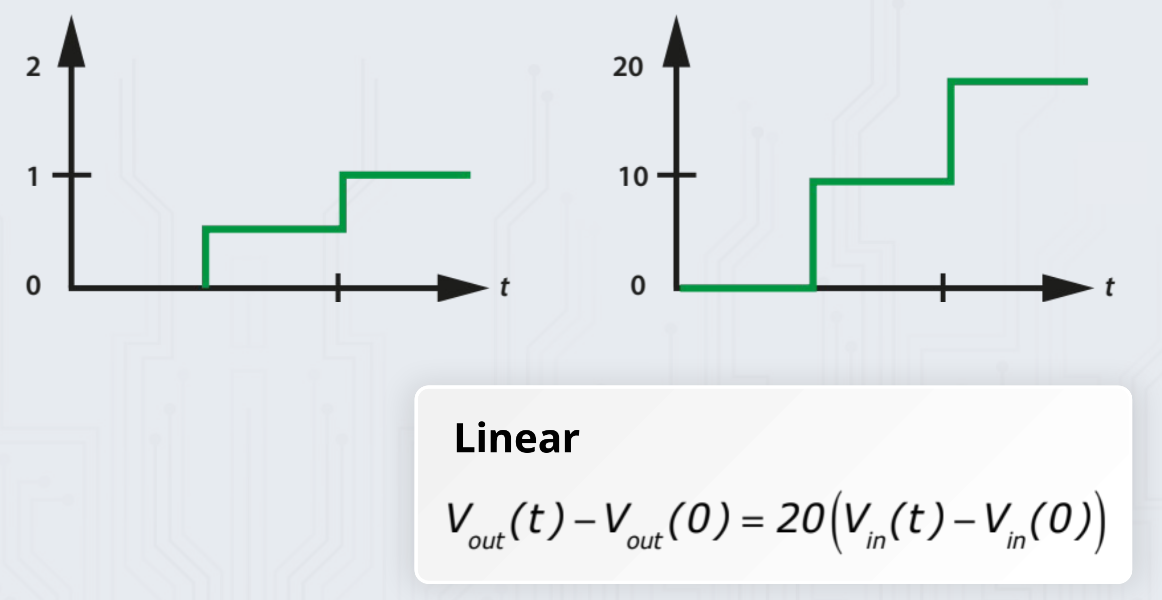
\includegraphics[height=15em]{./images/amplitude-linearity-stepwise-function.png}
\end{center}

\begin{center}
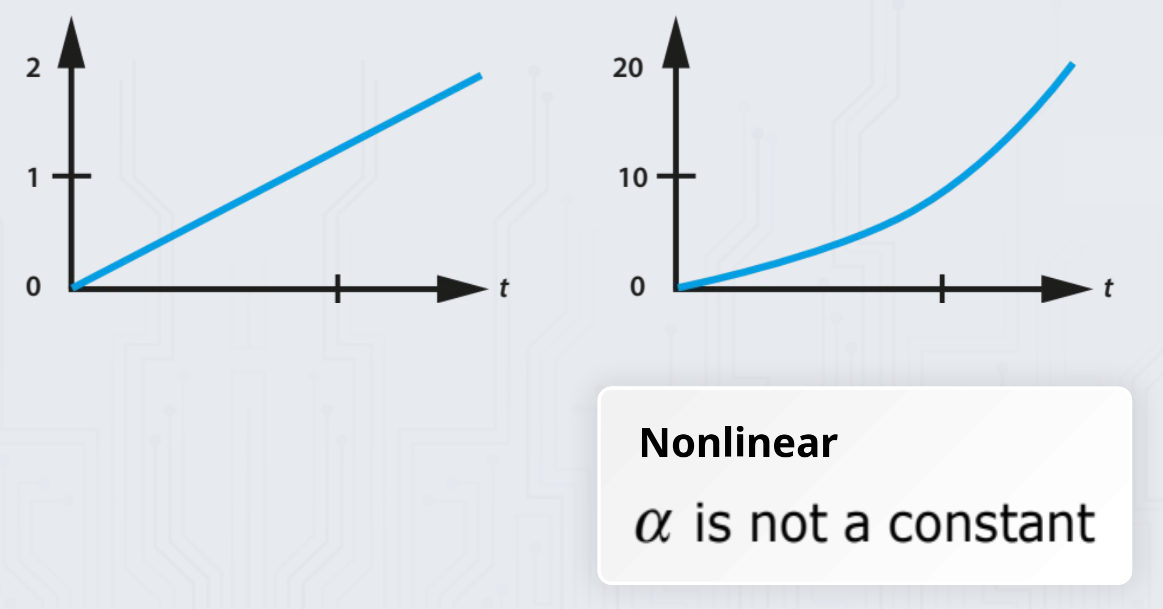
\includegraphics[height=15em]{./images/amplitude-nonlinearity-curve.png}
\end{center}

\begin{center}
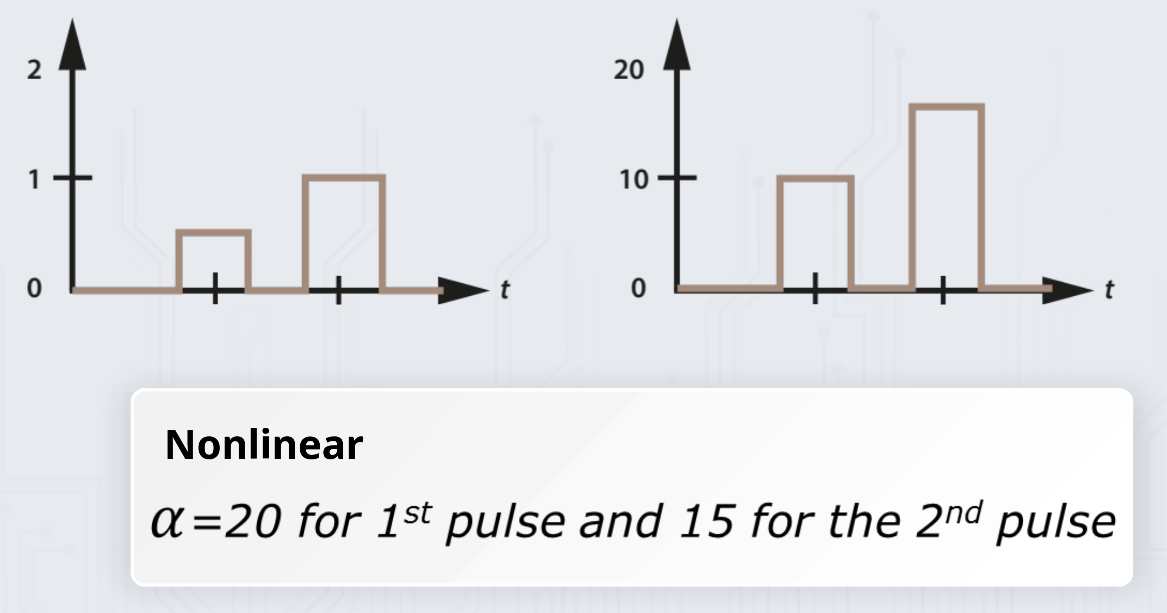
\includegraphics[height=15em]{./images/amplitude-nonlinearity-pulse.png}
\end{center}
\subsection{Period and frequency}
\label{sec:orgfd4b011}
\(T\) is the period in \textbf{seconds}, which is the inverse of frequency (\(f\) in \(\unit{Hz}\)).

\begin{center}
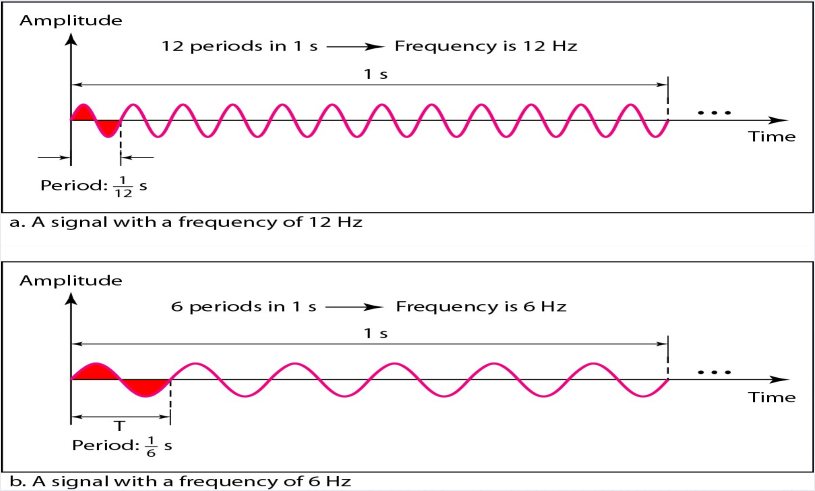
\includegraphics[width=.9\linewidth]{./images/period-and-frequency-images.png}
\end{center}
\subsection{Time and frequency domain}
\label{sec:orgff360e9}
Below are the time-domain and frequency-domain plots of a sine wave.

\begin{center}
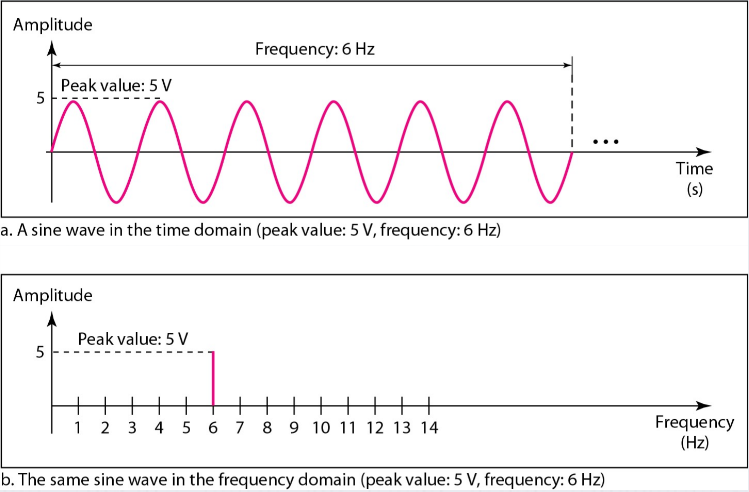
\includegraphics[width=.9\linewidth]{./images/time-domain-and-frequency-domain-images.png}
\end{center}
\subsection{Magnitude ratio (\(M\))}
\label{sec:orgab69ff3}
Magnitude ratio, which can be considered as the attenuation, is always less than 1, and is given by:
\[M(\omega) = \frac{1}{\sqrt{1 + (\omega \tau)^2}}\]

Where:
\begin{itemize}
\item \(M\) is the magnitude ratio
\item \(\omega\) is the angular frequency
\item \(\tau\) is the time constant
\end{itemize}
\subsection{Dynamic error (\(\delta\))}
\label{sec:org0f12225}
A dynamic error for a first order system is always less than 1, and is given by:
\[\delta(\omega) = 1 - M(\omega)\]

Where:
\begin{itemize}
\item \(\delta\) is the dynamic error
\item \(M\) is magnitude ratio
\end{itemize}
\subsection{Radicand}
\label{sec:org8e19fa3}
Radicand is the quantity inside the square root sign. For example, the radicand of \(\sqrt{3}\) is 3, and the radicand of \(\sqrt{x^2 + 2bx + b^2}\) is \(x^2 + 2bx + b^2\).
\subsection{Cut-off frequency (\(f_c\))}
\label{sec:org4ed35b0}
\[f_c = \frac{1}{2 \pi RC}\]

Where:
\begin{itemize}
\item \(f_c\) is the cut-off frequency
\item \(R\) is the resistance of the resistor (\(\unit{\ohm}\))
\item \(C\) is the capacitance of the capacitor (\(\unit{F}\))
\end{itemize}
\subsubsection{Time constant estimate (\(\tau\))}
\label{sec:org74e37de}
\[\tau \approx \frac{1}{f_c}\]

Where:
\begin{itemize}
\item \(\tau\) is the time constant
\item \(f_c\) is the cut-off frequency
\end{itemize}
\subsection{Frequency response of a filter (\(M\))}
\label{sec:org7d5ad46}
\[M(\omega) = \frac{1}{\sqrt{1 + \left(\frac{f}{f_c} \right)^2}}\]

Where:
\begin{itemize}
\item \(M\) is the frequency response
\item \(f\) is the target frequency
\item \(f_c\) is the cut-off frequency of the filter
\end{itemize}
\subsection{Common mode rejection ratio (CMRR)}
\label{sec:org184e67d}
\begin{itemize}
\item Common mode rejection ratio (CMRR) is the ratio of the different mode gain to the common mode gain.
\item The difference mode gain is the amplification factor for the difference between the input signals.
\item The common mode gain is the amplification factor for the average of the input signals.
\item For an ideal difference amplifier, the common mode gain is 0, implying an infinite common mode rejection ratio.
\item It is desirable to minimise the common mode gain to suppress signals such as noise that are common to both inputs.
\end{itemize}
\subsection{Analogue-to-digital (A/D) conversion}
\label{sec:orgb5c13fc}
\begin{itemize}
\item An electronic integrated circuit which transforms a signal from analogue (continuous) to digital (discrete) form.
\item Analogue signals are directly measurable quantities.
\item Digital signals only have two states. For the digital computer, we refer to the binary states: 0 and 1.
\end{itemize}
\subsection{Dithering}
\label{sec:orgac21a90}
Dithering is a form of noise that is intentionally applied to randomise quantisation error.
\subsection{Transducers}
\label{sec:orgc788fcf}
Transducers convert one form of energy into another, and it is not necessary to perform a measurement.
\subsection{Sensors}
\label{sec:org558aab8}
Sensors produce an output signal, which is typically electrical, for the purpose of sensing a physical phenomenon.
\subsection{Sensor classification}
\label{sec:org9235efd}
\begin{itemize}
\item Analogue vs digital
\begin{itemize}
\item Light on and off switch vs light dimmer.
\end{itemize}
\item Passive vs active
\begin{itemize}
\item Passive sensors do not require external an external power supply, and they draw energy from the input signal itself.
\end{itemize}
\item Null versus deflection type
\begin{itemize}
\item Null type sensors counteract any deflection due to the measured quantity using an opposing calibrated force.
\end{itemize}
\item Subject of measurement
\begin{itemize}
\item Mechanical, optical, thermal, etc.
\end{itemize}
\end{itemize}
\subsection{Instrumentation systems}
\label{sec:org1fbe74f}
\begin{itemize}
\item Sensing module, which can be mechanical, thermal, optical, pyrolytic, piezoelectric, etc.
\item Conversion module to convert from analogue to digital.
\item Pre-processing, which is a module that manipulates the variables.
\item Data transmission, which can be wired or wireless, transferred over the internet, etc.
\item Presentation or storage to the user.
\end{itemize}
\subsection{Input}
\label{sec:orgd4100e0}
Input is the stimulus. Some examples include temperature, pressure, and strain.
\subsection{Output}
\label{sec:org69a7894}
The output is usually an electrical signal, which is defined using voltage, current, frequency, phase, etc.
\subsection{Sensitivity (\(S\))}
\label{sec:org947b0ff}
The sensitivity is defined as:
\[S = \frac{\text{Output variation}}{\text{Input variation}}\]

It is also the slope of the graph of the output (\(f(x)\)) against the input (\(x\)).
\[S = \frac{df}{dx}\]
\subsection{Resolution}
\label{sec:org1f68416}
The resolution is the minimum change of the input that can be reliably detected. It is limited by noise, bit-conversion, and many other things.
\subsection{Accuracy}
\label{sec:org17e54cd}
The accuracy is the difference of the measurement from the true value.

 \newpage
\subsection{Repeatability}
\label{sec:org36f06a9}
Repeatability is how well a system or device can reproduce an outcome in unchanged conditions.

\begin{center}
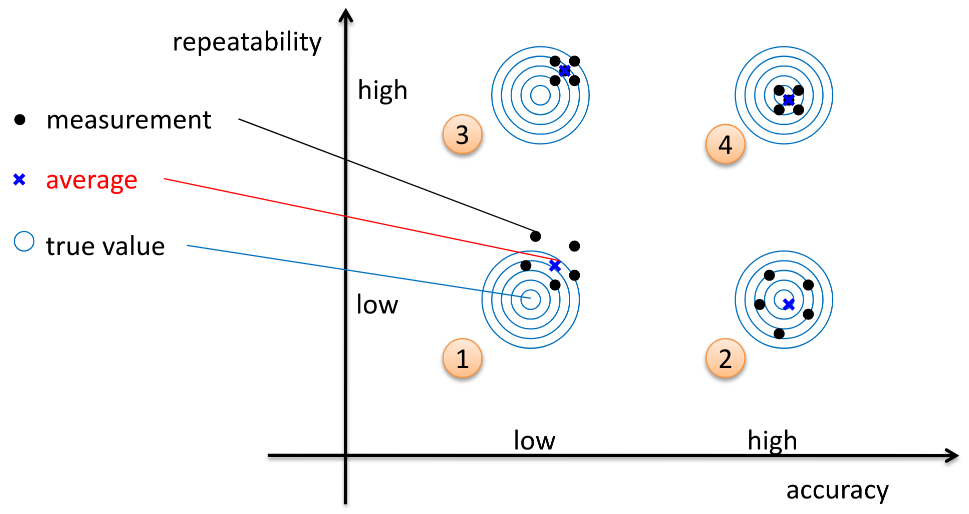
\includegraphics[width=.9\linewidth]{./images/repeatability-and-accuracy.png}
\end{center}
\subsection{Types of instrument errors}
\label{sec:org679a63a}

\subsubsection{Nonlinearity}
\label{sec:org664c960}
\begin{center}
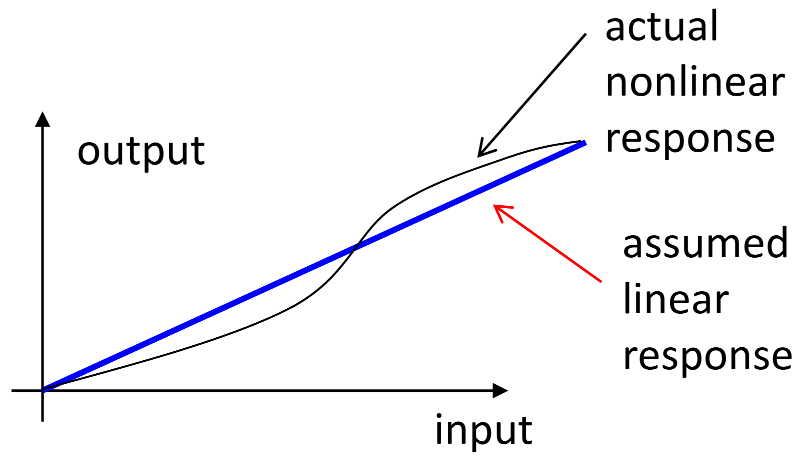
\includegraphics[width=.9\linewidth]{./images/instrument-error-nonlinearity.png}
\end{center}
\subsubsection{Hysteresis}
\label{sec:org0165736}
\begin{center}
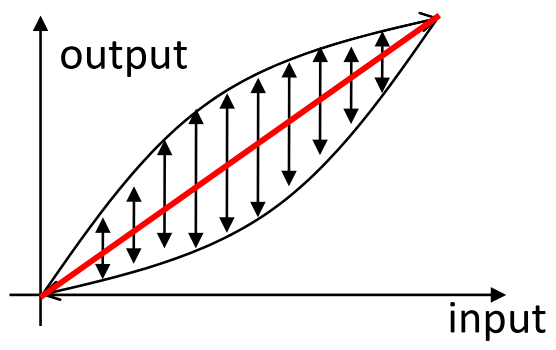
\includegraphics[width=.9\linewidth]{./images/instrument-error-hysteresis.png}
\end{center}
\subsubsection{Sensitivity error}
\label{sec:orgc41435b}
\begin{center}
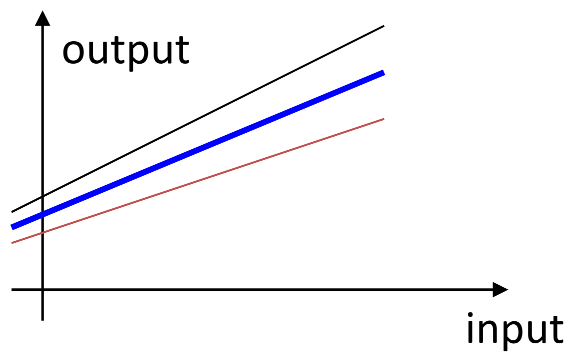
\includegraphics[width=.9\linewidth]{./images/instrument-error-sensitivity-error.png}
\end{center}
\subsubsection{Zero-shift error}
\label{sec:org4a2c988}
\begin{center}
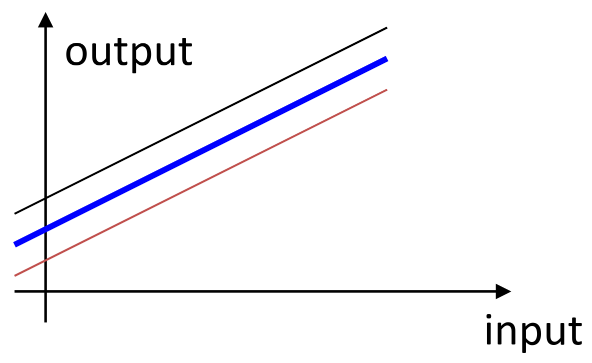
\includegraphics[width=.9\linewidth]{./images/instrument-error-zero-shift-error.png}
\end{center}
\subsection{Lorentz's law}
\label{sec:org368999d}
\begin{center}
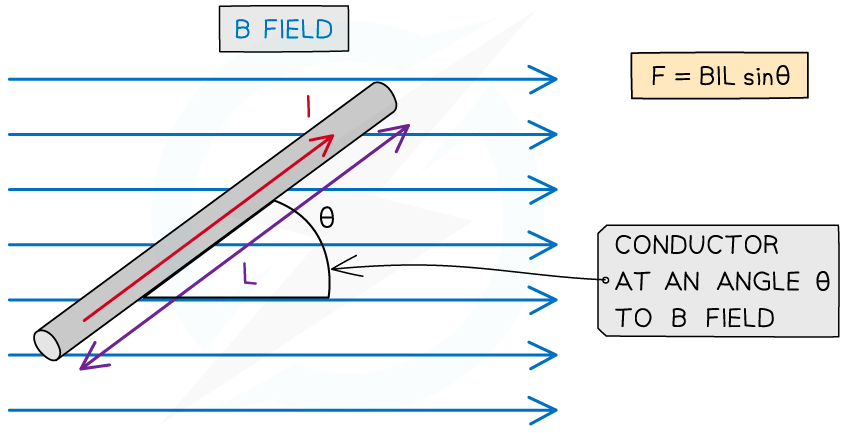
\includegraphics[height=12em]{./images/lorentz-law-diagram.png}
\end{center}

\[\vec{F} = (\vec{i} \times \vec{B}) L\]
\[F = || \vec{F} || BiL \sin \theta\]

Where:
\begin{itemize}
\item \(\vec{F}\) is the magnetic force
\item \(\vec{i}\) is the current
\item \(\vec{B}\) is the magnetic field
\item \(L\) is the length of the wire
\end{itemize}
\subsection{Faraday's law}
\label{sec:org1cc2f02}
\begin{center}
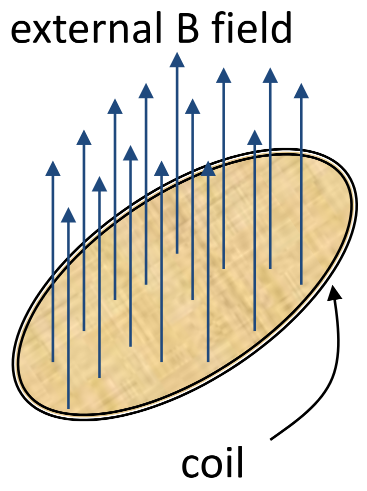
\includegraphics[height=20em]{./images/faradays-law-diagram.png}
\end{center}

\[emf = E = -\frac{d \Phi}{dt}\]
\[\Phi \triangleq \int_{\Sigma} \vec{B} \, d \vec{\Sigma}\]

Where:
\begin{itemize}
\item \(emf\) is the electromotive force
\item \(\Phi\) is the magnetic flux
\item \(\Sigma\) is the surface whose boundary coincides with the coil
\begin{itemize}
\item It is not \textbf{uniquely defined} but \(\text{div } B = 0\), which means the integral only depends on the boundary.
\end{itemize}
\end{itemize}

 \newpage
\section{Fourier series representation of signals}
\label{sec:org0a13483}
\begin{itemize}
\item Any periodic signal can be represented by a combination of an infinite number of sinusoid terms.
\item Easy and standardised way to deal with any periodic signals (simple or complicated) using sine and cosine terms.
\item In addition to time domain analysis, frequency domain analysis helps to gain insights of the signals which are fundamental to signal processing, and other mechatronics applications.
\item To study bandwidth and phase linearity, which are applied to frequency components of an input signal, it is necessary to review the Fourier series representation of a signal.
\item Any periodical waveform can be represented as an infinite series of sine and cosine waveforms of different amplitudes and frequencies.
\item Summing up this infinite series gives the original periodical waveform.
\item Practically, a finite number of the sine and cosine waveforms can adequately represent a periodical waveform.
\end{itemize}
\subsection{Fundamental frequency}
\label{sec:orgeeed551}
Let \(\omega_0\) be the fundamental of first (lowest) harmonic frequency defined as:
\[\omega_0 = \frac{2\pi}{T} = 2 \pi f_0\]

Where:
\begin{itemize}
\item \(\omega_0\) is the fundamental angular frequency
\item \(T\) is the period
\item \(f_0\) is the fundamental frequency in \(\unit{Hz}\)
\end{itemize}

The other sine and cosine waveforms have frequencies of integer multiples of \(\omega_0\).

 \newpage
\subsection{Fourier series representation of a periodical waveform}
\label{sec:orga0fcf3c}
The Fourier series representation of a periodical waveform \(f(t)\) is:
\[F(t) = C_0 + \sum_{n = 1}^{\infty} A_n \cos (n \omega_0 t) + \sum_{n = 1}^{\infty} B_n \sin (n \omega_0 t)\]

Where:
\begin{itemize}
\item \(C_0\) is the DC component of the signal, i.e. the non-periodical part of the waveform, given by:
\[C_0 = \frac{1}{T} \int_0^T f(t) \, dt = \frac{A_0}{2}\]

Where:
\begin{itemize}
\item \(T\) is the period
\item \(f(t)\) is the periodical waveform
\item \(t\) is the time
\item \(A_0\) is the initial amplitude of the waveform
\end{itemize}

\item \(A_n\) is given by:
\[A_n = \frac{2}{T} \int_0^T f(t) \cos (n \omega_0 t) \, dt\]

Where:
\begin{itemize}
\item \(T\) is the period
\item \(\omega_0\) is the fundamental angular frequency
\item \(t\) is the time
\item \(n\) is just a number
\end{itemize}

\item \(B_n\) is given by:
\[B_n = \frac{2}{T} \int_0^T f(t) \sin (n \omega_0 t) \, dt\]

Where:
\begin{itemize}
\item \(T\) is the period
\item \(\omega_0\) is the fundamental angular frequency
\item \(t\) is the time
\item \(n\) is just a number
\end{itemize}
\end{itemize}

Note that \(C_0\) is the average value of the waveform over its period.
\subsubsection{In general}
\label{sec:org6508395}
Given:
\[C_n = \sqrt{A_n^2 + B_n^2}\]
\[\phi_n = - \arctan \left(\frac{B_n}{A_n} \right)\]

Then:
\begin{align*}
F(t) &= C_0 + \sum_{n = 1}^{\infty} \left(A_n \cos (n \omega_0 t) + B_n (\sin n \omega_0 t) \right) \\
&= C_0 + \sum_{n = 1}^{\infty} \sqrt{A_n^2 + B_n^2} \left(\frac{A_n}{\sqrt{A_n^2 + B_n^2}} \cos (n \omega_0 t) + \frac{B_n}{\sqrt{A_n^2 + B_n^2}} \sin (n \omega_0 t) \right) \\
&= C_0 + \sum_{n = 1}^{\infty} C_n \left(\cos (\phi_n) \cos(n \omega_0 t) - \sin(\phi_n) \sin(n \omega_0 t) \right) \\
&= C_0 + \sum_{n = 1}^{\infty} C_n \cos (n \omega_0 t + \phi_n)
\end{align*}

\[\phi_n = - \arctan \left(\frac{B_n}{A_n} \right)\]
\[\cos (\phi_n) = \frac{A_n}{\sqrt{A_n^2 + B_n^2}}\]
\[\sin (\phi_n) = - \frac{B_n}{\sqrt{A_n^2 + B_n^2}}\]

 \newpage
\subsubsection{Sine form}
\label{sec:org71cb051}
Given:
\[C_n = \sqrt{A_n^2 + B_n^2}\]
\[\phi_n^* = \arctan \left(\frac{A_n}{B_n} \right)\]

Then:
\begin{align*}
F(t) &= C_0 + \sum_{n = 1}^{\infty} \left(A_n \cos (n \omega_0 t) + B_n (\sin n \omega_0 t) \right) \\
&= C_0 + \sum_{n = 1}^{\infty} \sqrt{A_n^2 + B_n^2} \left(\frac{A_n}{\sqrt{A_n^2 + B_n^2}} \cos (n \omega_0 t) + \frac{B_n}{\sqrt{A_n^2 + B_n^2}} \sin (n \omega_0 t) \right) \\
&= C_0 + \sum_{n = 1}^{\infty} C_n \left(\sin (\phi_n^*) \cos (n \omega_0 t) + \cos (\phi_n^*) \sin (n \omega_0 t) \right) \\
&= C_0 + \sum_{n = 1}^{\infty} C_n \sin (n \omega_0 t + \phi_n^*)
\end{align*}

\[\phi_n^* = \arctan \left(\frac{A_n}{B_n} \right)\]
\[\sin (\phi_n^*) = \frac{A_n}{\sqrt{A_n^2 + B_n^2}}\]
\[\cos (\phi_n^*) = \frac{B_n}{\sqrt{A_n^2 + B_n^2}}\]

 \newpage
\subsubsection{Example: Square waveform with period T}
\label{sec:org5c3744f}
The square waveform is defined as:
\begin{displaymath}
f(t) = \begin{cases}
1 & 0 \le t \le \frac{T}{2} \\
-1 & \frac{T}{2} \le t \le T \\
\end{cases}
\end{displaymath}

Then:
\[A_n = 0\]
\begin{align*}
B_n &= \frac{2}{T} \left(\int_0^{\frac{T}{2}} \sin (n \omega_0 t) \, dt - \int_{\frac{T}{2}}^T \sin (n \omega_0 t) \, dt \right) \\
&= \frac{2}{T} \left(- \left.\frac{1}{n \omega_0} \cos (n \omega_0 t) \right|_0^{\frac{T}{2}} + \left. \frac{1}{n \omega_0} \cos (n \omega_0 t) \right|_{\frac{T}{2}}^T \right) \\
&= \frac{2}{n \pi} (1 - \cos (n \pi)) \\
&= \begin{cases}
\frac{4}{n \pi} & \textit{if } n \textit{ is odd} \\
0 & \textit{if } n \textit{ is even} \\
\end{cases}
\end{align*}

Therefore:
\begin{align*}
F(t) &= \frac{4}{\pi} \sin(\omega_0 t) + \frac{4}{3 \pi} \sin(3 \omega_0 t) + \frac{4}{5 \pi} \sin (5 \omega_0 t) + \cdots \\
&= \sum_{n = 1}^{\infty} \frac{4}{(2n - 1) \pi} \sin ((2n - 1) \omega_0 t)
\end{align*}
\subsubsection{Representation of a square wave}
\label{sec:org912bd5b}
\begin{center}
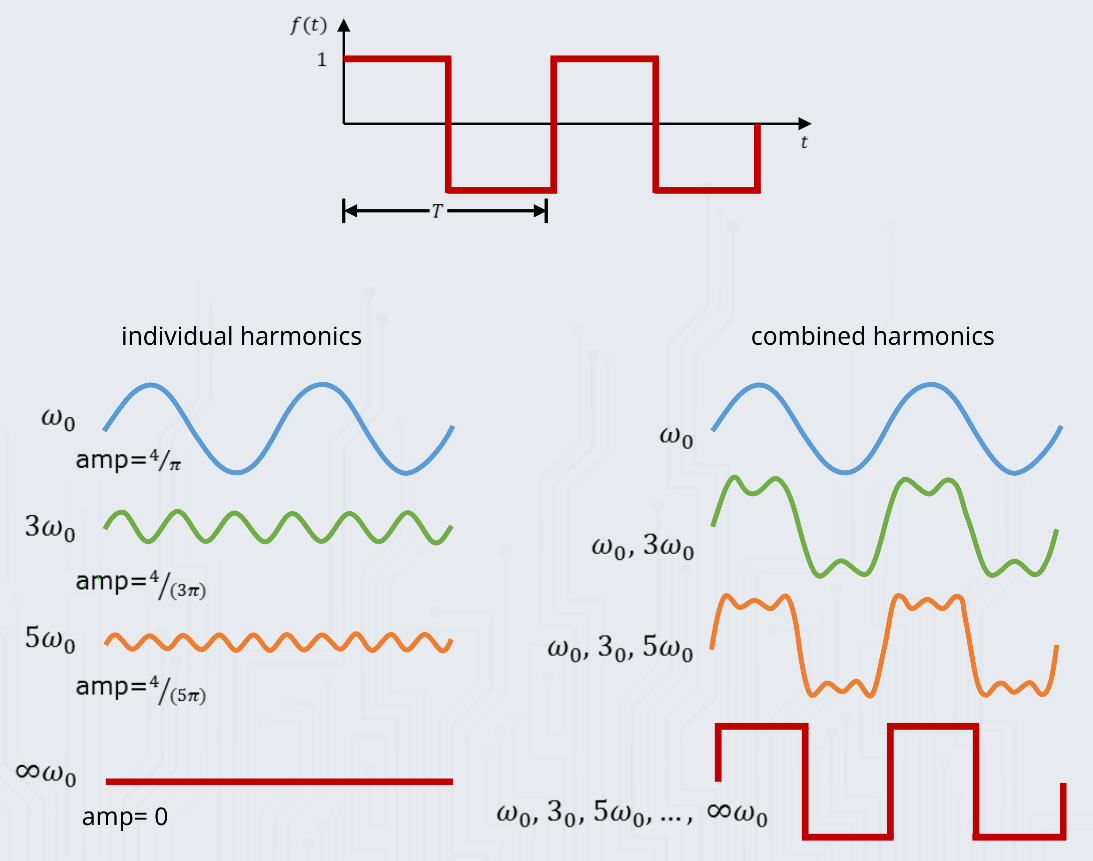
\includegraphics[width=.9\linewidth]{./images/square-wave-fourier-series-representation.png}
\end{center}

 \newpage
\subsubsection{Plotting the frequency spectrum of a waveform}
\label{sec:org979f2b3}
When plotting the frequency spectrum for a signal represented by a Fourier series, use the signal amplitude generated from the equation below:
\[F(t) = C_0 + \sum_{n = 1}^{\infty} C_n \cos (n \omega_0 t + \phi_n)\]

\begin{center}
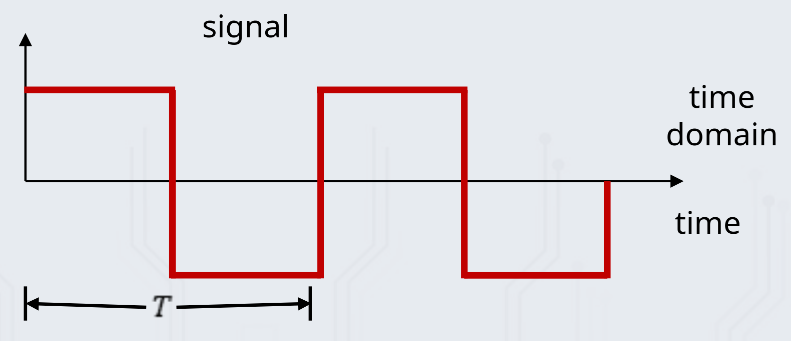
\includegraphics[width=.9\linewidth]{./images/square-wave-signal.png}
\end{center}

For the square wave above:
\[F(t) = \frac{4}{\pi} \sin(\omega_0 t) + \frac{4}{3 \pi} \sin (3 \omega_0 t) + \frac{4}{5 \pi} \sin (5 \omega_0 t) + \cdots\]

\begin{center}
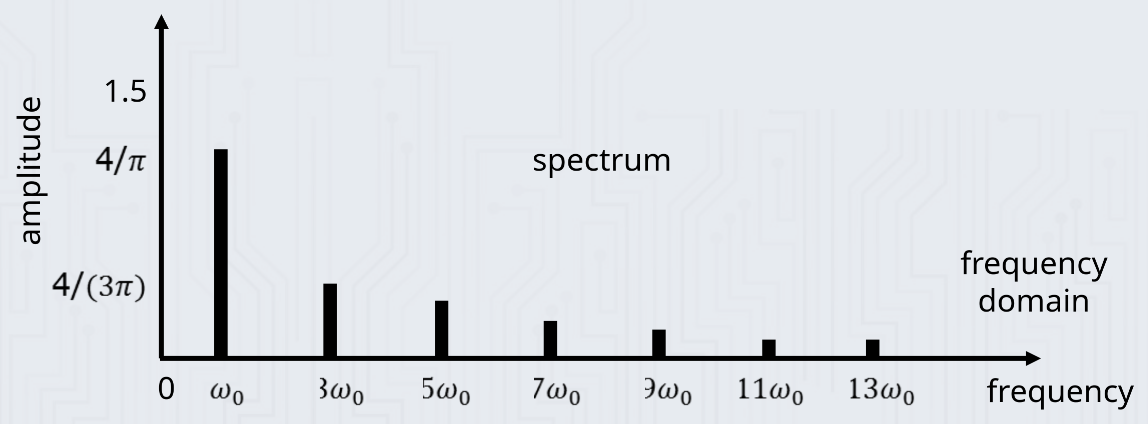
\includegraphics[width=.9\linewidth]{./images/square-wave-signal-frequency-spectrum.png}
\end{center}
\subsubsection{Time domain analysis}
\label{sec:orge3e998c}
\begin{center}
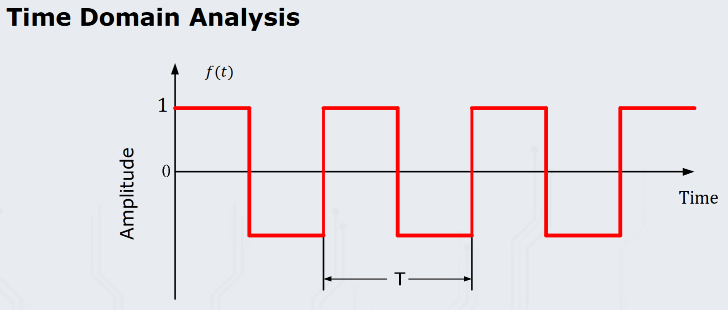
\includegraphics[width=.9\linewidth]{./images/time-domain-analysis.png}
\end{center}
\subsubsection{Frequency response analysis}
\label{sec:org2342022}
\begin{center}
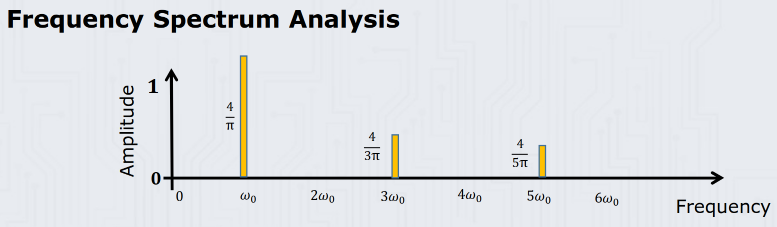
\includegraphics[width=.9\linewidth]{./images/frequency-spectrum-analysis.png}
\end{center}

 \newpage
\subsection{Even functions}
\label{sec:org80a8e81}
Even functions can solely be represented by cosine waves, i.e.
\[B_n = 0\]

Because \(\sin (n \omega_0 t)\) is an odd function, \(f(t) \cdot \sin(n \omega_0 t)\) is an odd function, hence:
\[B_n = \frac{2}{T} \int_{-\frac{T}{2}}^{\frac{T}{2}} f(t) \sin (n \omega_0 t) \, dt = 0\]

\[A_n = \frac{2}{T} \int_{-\frac{T}{2}}^{\frac{T}{2}} f(t) \cos (n \omega_0 t) \, dt = \frac{4}{T} \int_0^{\frac{T}{2}} f(t) \cos (n \omega_0 t) \, dt\]
\[F(t) = C_0 + A_1 \cos (1 \omega_0 t) + A_2 \cos (2 \omega_0 t) + A_3 \cos (2 \omega_0 t) + \ldots\]

\begin{center}
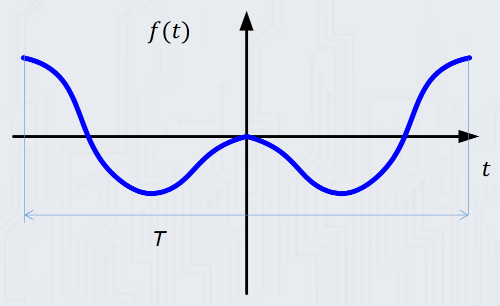
\includegraphics[width=.9\linewidth]{./images/even-function-fourier-series-representation.png}
\end{center}

 \newpage
\subsection{Odd functions}
\label{sec:orge6c6c21}
Even functions can solely be represented by sine waves, i.e.
\[C_0 = 0, \text{ and all } A_n = 0\]

Because \(\cos (n \omega_0 t)\) is an even function, \(f(t) \cdot \cos (n \omega_0 t)\) is an even function, hence:
\[A_n = \frac{2}{T} \int_{-\frac{T}{2}}^{\frac{T}{2}} f(t) \cos (n \omega_0 t) \, dt = 0\]
  \[C_0 = \frac{1}{T} \int_{-\frac{T}{2}}^{\frac{T}{2}} f(t) \, dt = 0\]

\[B_n = \frac{2}{T} \int_{-\frac{T}{2}}^{\frac{T}{2}} f(t) \sin (n \omega_0 t) \, dt = \frac{4}{T} \int_0^{\frac{T}{2}} f(t) \sin (n \omega_0 t) \, dt\]
\[F(t) = C_0 + B_1 \sin (1 \omega_0 t) + B_2 \sin (2 \omega_0 t) + B_3 \sin (3 \omega_0 t) + \ldots\]

\begin{center}
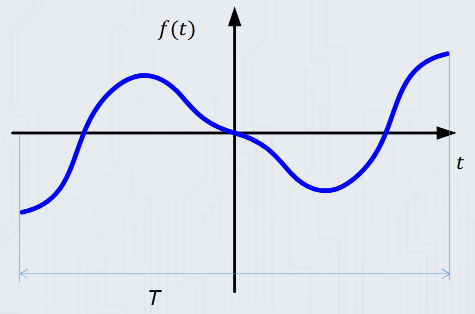
\includegraphics[width=.9\linewidth]{./images/odd-function-fourier-series-representation.png}
\end{center}

 \newpage
\subsection{Calculation of the Fourier coefficients}
\label{sec:orgac658f6}
Find the Fourier series for the following periodic waveform:
\begin{center}
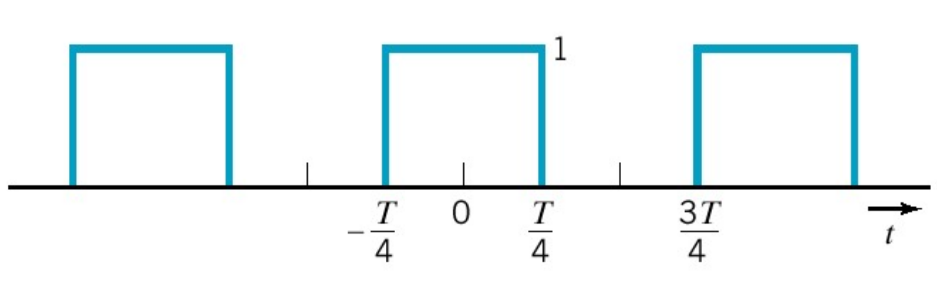
\includegraphics[width=.9\linewidth]{./images/even-square-wave-function.png}
\end{center}

Function:
\begin{displaymath}
f(t) = \begin{cases}
1, & t \in [-\frac{T}{4}, \frac{T}{4}] \\
0, & t \in [\frac{T}{4}, \frac{3T}{4}] \\
\end{cases}
\end{displaymath}

Periodic:
\[f(t + T) = f(t)\]
\[\text{Period} = T\]

Symmetry: Even-function
\[f(-t) = f(t)\]

The function is an even function, hence:
\[B_n = 0\]
\[C_0 = \frac{1}{T} \int_{-\frac{T}{4}}^{\frac{3T}{4}} f(t) \, dt = \frac{1}{T} \int_{-\frac{T}{4}}^{\frac{T}{4}} 1 \, dt = \frac{1}{2}\]
\begin{align*}
A_n &= \frac{2}{T} \int_{-\frac{T}{2}}^{\frac{T}{2}} f(t) \cos (n \omega_0 t) \, dt \\
&= \frac{4}{T} \int_0^{\frac{T}{2}} f(t) \cos (n \omega_0 t) \, dt \\
&= \frac{4}{T} \int_0^{\frac{T}{4}} 1 \cos (n \omega_0 t) \, dt \\
&= \frac{4}{n \pi \omega_0 T} \int_0^{\frac{T}{4}} \, d(\sin (n \omega_0 t)) \\
&= \frac{4}{n \pi \omega_0 t} \left(\sin (n \omega_0 \frac{T}{4} - 0) \right) \\
&= \frac{2}{n \pi} \sin \left(\frac{n \pi}{2} \right)
\end{align*}

The corresponding Fourier series is:
\[F(t) = \frac{1}{2} + \frac{2}{\pi} \cos \left(1 \cdot \frac{2 \pi}{T} \cdot t \right) - \frac{2}{3 \pi} \cos \left( 3 \cdot \frac{2 \pi}{T} \cdot t \right) + \frac{2}{5 \pi} \cos \left( 5 \cdot \frac{2 \pi}{T} \cdot t \right) - \frac{2}{7 \pi} \cos \left( 7 \cdot \frac{2 \pi}{T} \cdot t \right) + \ldots\]

\begin{center}
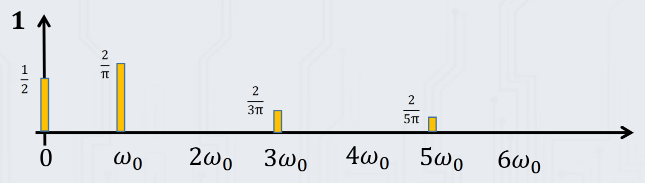
\includegraphics[width=.9\linewidth]{./images/caculation-of-the-fourier-series-frequency-spectrum-result.png}
\end{center}

 \newpage
\subsection{Square wave decomposition}
\label{sec:org2ff9701}

\subsubsection{Half square wave decomposition}
\label{sec:org6141c01}
\begin{center}
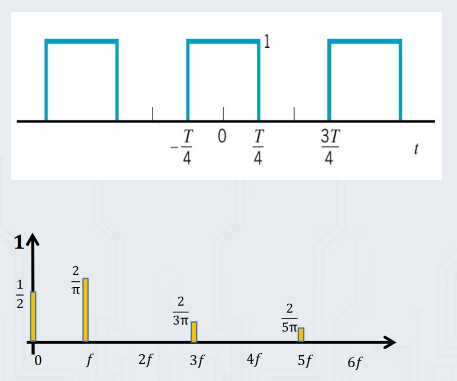
\includegraphics[width=.9\linewidth]{./images/half-square-wave-decomposition.png}
\end{center}

\[F(t) = \frac{1}{2} + \frac{2}{\pi} \cos \left(1 \cdot \frac{2 \pi}{T} \cdot t \right) - \frac{2}{3 \pi} \cos \left( 3 \cdot \frac{2 \pi}{T} \cdot t \right) + \frac{2}{5 \pi} \cos \left( 5 \cdot \frac{2 \pi}{T} \cdot t \right) - \frac{2}{7 \pi} \cos \left( 7 \cdot \frac{2 \pi}{T} \cdot t \right) + \ldots\]
\subsubsection{Full square wave decomposition}
\label{sec:orgee7b4ce}
\begin{center}
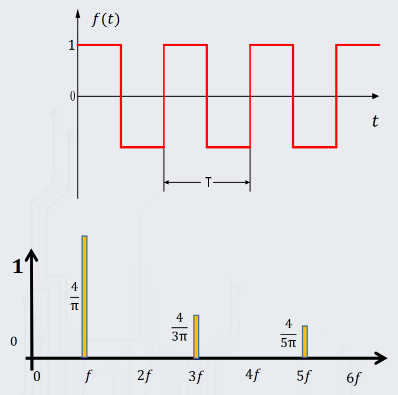
\includegraphics[width=.9\linewidth]{./images/full-square-wave-decomposition.png}
\end{center}

\[F(t) = \frac{4}{\pi} \sin(\omega_0 t) + \frac{4}{3 \pi} \sin (3 \omega_0 t) + \frac{4}{5 \pi} \sin (5 \omega_0 t) + \cdots\]

 \newpage
\subsection{Complex form of the Fourier series}
\label{sec:org0a8a428}
The standard Fourier series representation is given as:
\[F(t) = C_0 + \sum_{n = 1}^{\infty} (A_n \cos (n \omega_0 t) + B_n \sin (n \omega_0 t))\]

Using Euler's formulae:
\[\cos (n \omega_0 t) = \frac{e^{jn \omega_0 t} + e^{-jn \omega_0 t}}{2}\]
\[\sin (n \omega_0 t) = \frac{e^{jn \omega_0 t} + e^{-jn \omega_0 t}}{2j}\]

So:
\[e^{jn \omega_0 t} = \cos(n \omega_0 t) + j \sin{(n \omega_0 t)}\]
\[e^{-jn \omega_0 t} = \cos(n \omega_0 t) - j \sin{(n \omega_0 t)}\]

The \(n\)-th harmonic component can be expressed as:
\begin{align*}
&A_n \cos (n \omega_0 t) + B_n \sin(n \omega_0 t) \\
&= A_n \frac{e^{jn \omega_0 t} + e^{-jn \omega_0 t}}{2} + B_n \frac{e^{jn \omega_0 t} - e^{-jn \omega_0 t}}{2j} \\
&= A_n \frac{e^{jn \omega_0 t} + e^{-jn \omega_0 t}{2}} + -j B_n \frac{e^{jn \omega_0 t} - e^{-jn \omega_0 t}}{2} \\
&= \frac{A_n - j B_n}{2} e^{jn \omega_0 t} + \frac{A_n + j}{2} e^{-jn \omega_0 t}
\end{align*}

Denoting:
\[D_n = \frac{A_n - j B_n}{2}, \quad D_{-n} = \frac{A_n + j B_n}{2}\]
\[D_0 = \frac{A_0}{2}\]

\[A_n \cos (n \omega_0 t) + B_n \sin (n \omega_0 t) = D_n e^{jn \omega_0 t} + D_{-n} e^{-jn \omega_0 t}\]

Therefore, the Fourier series can be expressed as:
\[F(t) = D_0 + \sum_{n = 1}^{\infty} (D_n e^{jn \omega_0 t} + D_{-n} e^{-jn \omega_0 t}) = \sum_{n = -\infty}^{\infty} D_n e^{jn \omega_0 t}\]
\subsubsection{Coefficients}
\label{sec:org4651da8}
The coefficients \(D_n\) can be evaluated in the following manner:
\begin{align*}
D_n &= \frac{(A_n - j B_n)}{2} \\
&= \frac{1}{T} \int_{-\frac{T}{2}}^{\frac{T}{2}} f(t) \cos (n \omega_0 t) \, dt - \frac{j}{T} \int_{-\frac{T}{2}}^{\frac{T}{2}} f(t) \sin(n \omega_0 t) \, dt \\
&= \frac{1}{T} \int_{-\frac{T}{2}}^{\frac{T}{2}} f(t) (\cos (n \omega_0 t) - j \sin (n \omega_0 t)) \, dt \\
&= \frac{1}{T} \int_{-\frac{T}{2}}^{\frac{T}{2}} f(t) e^{-jn \omega_0 t} \, dt
\end{align*}

The coefficients \(D_{-n}\) can be evaluated in the following manner:
\begin{align*}
D_{-n} &= \frac{(A_n + j B_n)}{2} \\
&= \frac{1}{T} \int_{-\frac{T}{2}}^{\frac{T}{2}} f(t) \cos (n \omega_0 t) \, dt + \frac{j}{T} \int_{-\frac{T}{2}}^{\frac{T}{2}} f(t) \sin(n \omega_0 t) \, dt \\
&= \frac{1}{T} \int_{-\frac{T}{2}}^{\frac{T}{2}} f(t) (\cos (n \omega_0 t) + j \sin (n \omega_0 t)) \, dt \\
&= \frac{1}{T} \int_{-\frac{T}{2}}^{\frac{T}{2}} f(t) e^{jn \omega_0 t} \, dt
\end{align*}

Note that \(D_{-n}\) is the complex conjugate of \(D_n\):
\[D_n = \frac{(A_n - j B_n)}{2}\]
\[D_{-n} = \frac{(A_n + j B_n)}{2}\]

So the Fourier series decomposition has the \(D_n\) in complex form:
\[D_n = \frac{1}{T} \int_{- \frac{T}{2}}^{\frac{T}{2}} f(t) e^{-jn \omega_0 t} \, dt \quad n = 0, \pm 1, \pm 2, \ldots\]

We have the complex form of the Fourier series:
\[F(t) = \sum_{n = - \infty}^{\infty} D_n e^{jn \omega_0 t}\]
\subsection{Regular form vs complex form}
\label{sec:orgea36c1b}

\subsubsection{Regular form}
\label{sec:org9793a00}
\[A_n = \frac{2}{T} \int_0^T f(t) \cos (n \omega_0 t) \, dt \quad n = 1, 2, 3, \ldots\]
\[B_n = \frac{2}{T} \int_0^T f(t) \sin (n \omega_0 t) \, dt \quad n = 1, 2, 3, \ldots\]
\[F(t) = C_0 + \sum_{n = 1}^{\infty} A_n \cos (n \omega_0 t) + B_n \sin(n \omega_0 t)\]
\subsubsection{Complex form}
\label{sec:orge924d3e}
\[D_n = \frac{1}{T} \int_{-\frac{T}{2}}^{\frac{T}{2}} f(t) e^{-jn \omega_0 t} \, dt\]
\[n = 0, \pm 1, \pm 2, \ldots\]
\[F(t) = \sum_{n = - \infty}^{\infty} D_n e^{jn \omega_0 t}\]
\subsection{Cosine-only form vs complex form}
\label{sec:org7cf8ae8}

\subsubsection{Cosine-only form}
\label{sec:org257aa60}
\[C_n = \sqrt{A_n^2 + B_n^2}\]
\[\phi_n = - \arctan \left(\frac{B_n}{A_n} \right)\]
\[F(t) = C_0 + \sum_{n = 1}^{\infty} C_n \cos (n \omega_0 t + \phi_n)\]

\[A_{-n} = \frac{2}{T} \int_0^t f(t) \cos (-n \omega_0 t) \, dt = A_n\]
\[B_{-n} = \frac{2}{T} \int_0^t f(t) \sin (-n \omega_0 t) \, dt = -B_n\]
\[C_n = \sqrt{A_{-n}^2 + B_{-n}^2} = \sqrt{A_n^2 + B_n^2} = C_n\]
\[\phi_{-n} = \arctan \left(\frac{B_{-n}}{A_{-n}} \right) = \arctan \frac{B_{n}}{A_n} = - \phi_n\]
\[F(t) = C_0 + \frac{1}{2} \sum_{n = -\infty, n \ne 0}^{\infty} C_n \cos(n \omega_0 t + \phi_n)\]
\subsubsection{Complex form}
\label{sec:org48d8346}
\[D_n = \frac{1}{T} \int_{-\frac{T}{2}}^{\frac{T}{2}} f(t) e^{-jn \omega_0 t} \, dt\]
\[n = 0, \pm 1, \pm 2, \ldots\]
\[F(t) = \sum_{n = - \infty}^{\infty} D_n e^{jn \omega_0 t}\]
\subsection{Complex Fourier series decomposition}
\label{sec:org01fc219}
\begin{center}
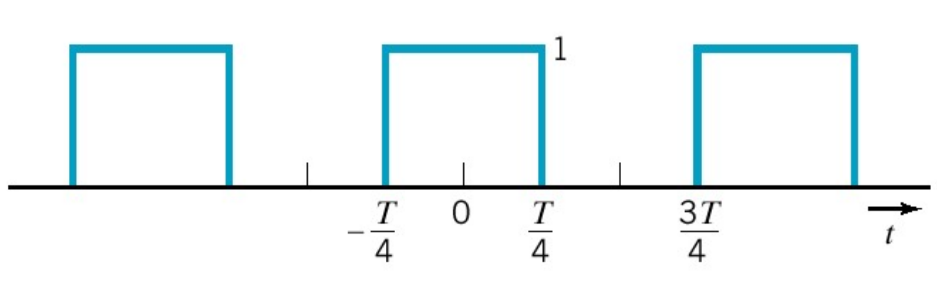
\includegraphics[width=.9\linewidth]{./images/even-square-wave-function.png}
\end{center}

Using \(nw \omega_0 = m\):
\begin{align*}
D_n &= \frac{1}{T} \int_{-\frac{T}{2}}^{\frac{T}{2}} f(t) e^{-jn \omega_0 t} \, dt \\
&= \frac{1}{T} \int_{-\frac{T}{4}}^{\frac{T}{4}} 1 e^{-mt} \, dt \\
&= \left. \frac{1}{-mT} e^{-mt} \right|_{-\frac{T}{4}}^{\frac{T}{4}} \\
&= - \frac{1}{mT} \left(e^{\frac{-mT}{4}} - e^{\frac{mT}{4}} \right)
\end{align*}

Using Euler's formulae:
\[\cos (n \omega_0 t) = \frac{e^{jn \omega_0 t} + e^{-jn \omega_0 t}}{2}\]
\[\sin (n \omega_0 t) = \frac{e^{jn \omega_0 t} + e^{-jn \omega_0 t}}{2j}\]

We have:
\begin{align*}
D_n &= \frac{1}{-in 2 \pi} \left(e^{\frac{in \pi}{2}} - e^{\frac{in}{2}} \right) \\
&= \frac{e^{\frac{in \pi}{2}} - e^{\frac{in \pi}{2}}}{2j} \frac{1}{\pi} \\
&= \frac{\sin \left(\frac{n \pi}{2} \right)}{n \pi} \\
D_{-n} &= \frac{\sin \left(\frac{- n \pi}{2} \right)}{- n \pi} \\
&= D_n
\end{align*}

To find \(D_0\):
\[D_0 = \frac{1}{T} \int_{-\frac{T}{4}}^{\frac{T}{4}} 1 \, dt = \frac{1}{2}\]

The square signal can be decomposed in complex form:
\begin{align*}
F(t) &= \sum_{n = -\infty}^{\infty} D_n e^{jn \omega_0 t} \\
&= D_0 + \sum_{n = 1}^{\infty} D_n (e^{jn \omega_0 t} + e^{-jn \omega_0 t}) \\
&= D_0 + \sum_{n = 1}^{\infty} 2 D_n \frac{e^{jn \omega_0 t} + e^{-jn \omega_0 t}}{2} \\
&= \frac{1}{2} + \sum_{n = 1}^{\infty} 2 \frac{\sin \left(\frac{n \pi}{2} \right)}{n \pi} \cos (n \omega_0 t)
\end{align*}

Setting \(\omega_0 = \frac{2 \pi}{T}\), the result is the same as the decomposition using the regular Fourier series:
\[F(t) = \frac{1}{2} + \frac{2}{\pi} \cos \left(1 \cdot \frac{2 \pi}{T} \cdot t \right) - \frac{2}{3 \pi} \cos \left( 3 \cdot \frac{2 \pi}{T} \cdot t \right) + \frac{2}{5 \pi} \cos \left( 5 \cdot \frac{2 \pi}{T} \cdot t \right) - \frac{2}{7 \pi} \cos \left( 7 \cdot \frac{2 \pi}{T} \cdot t \right) + \ldots\]

 \newpage
\subsection{Signal reconstruction}
\label{sec:orgbb3bc31}
Given:
\begin{itemize}
\item DC \(C_0\)
\item The all harmonic amplitude: \(A_n \text{ and } B_n, n = 1, 2, \ldots, N\)
\item The fundamental frequency \(\omega_0\)
\end{itemize}

We can reconstruct the signal by using either one of the following:
\[F(t) = C_0 + \sum_{n = 1}^{\infty} (A_n \cos (n \omega_0 t) + B_n \sin (n \omega_0 t))\]
\[F(t) = \sum_{n = - \infty}^{\infty} D_n e^{jn \omega_0 t}\]
\subsection{Signal approximation}
\label{sec:orgc988080}
Given:
\begin{itemize}
\item DC \(C_0\)
\item The all harmonic amplitude: \(A_n \text{ and } B_n, n = 1, 2, \ldots, N\)
\item The fundamental frequency \(\omega_0\)
\end{itemize}

We can approximate the signal by \(S_N (t)\):
\[F(t) = \sum_{n = - N}^{N} D_n e^{jn \omega_0 t}\]

 \newpage
\subsubsection{Approximation error}
\label{sec:org20ccec6}
A practical calculation of the Fourier series requires that we truncate the series to a finite number of terms.
\[f(t) \approxeq \sum_{n = - N}^{N} D_n e^{jn \omega_0 t} = S_N (t)\]

The error for \(N\) terms is:
\[\varepsilon (t) = f(t) - S_N (t)\]

The use the mean-square error (MSE) defined as:
\[\text{MSE} = \frac{1}{T} \int_0^T \varepsilon^2 (t) \, dt\]

MSE is minimum when \(D_n\) is equal to the Fourier series' coefficients.
\begin{center}
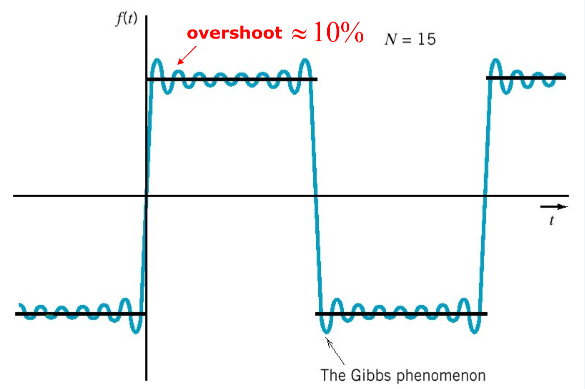
\includegraphics[width=.9\linewidth]{./images/approximation-error-graph.png}
\end{center}

 \newpage
\subsection{Amplitude and phase}
\label{sec:orgfc79e78}
Based on the cosine form of the Fourier series:
\[F(t) = C_0 + \sum_{n = 1}^{\infty} A_n \cos (n \omega_0 t + \phi_n)\]

A periodic waveform can be represented by an infinite series of cosine of \textbf{single amplitude} and \textbf{phase}.

\[\text{Single amplitude: } C_n = \sqrt{A_n^2 +B_n^2}\]
\[\text{Phase (angle): } \phi_n = - \arctan \left(\frac{B_n}{A_n} \right)\]
\subsection{Fourier spectrum}
\label{sec:org1a2fba4}

\subsubsection{Amplitude spectrum}
\label{sec:org930fc56}
\begin{center}
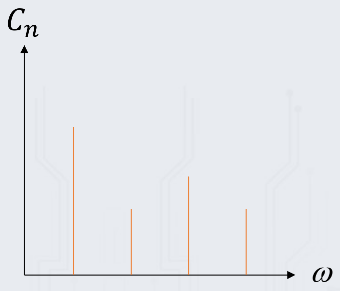
\includegraphics[width=.9\linewidth]{./images/amplitude-spectrum.png}
\end{center}
\subsubsection{Phase spectrum}
\label{sec:org24fc783}
\begin{center}
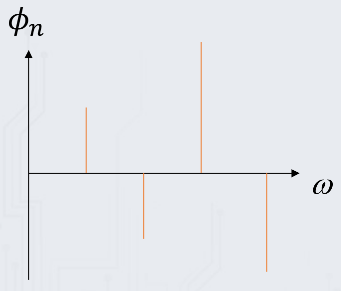
\includegraphics[width=.9\linewidth]{./images/phase-spectrum.png}
\end{center}
\subsubsection{Amplitude, frequency and phase}
\label{sec:orgdab77b0}
\begin{itemize}
\item \textbf{DC}: \(C_0\) is the average value of \(f(t)\)
\item The \(n^{th}\) \textbf{harmonic amplitude}: \(C_n\)
\item The \textbf{fundamental frequency}: \(\omega_0\)
\item The \(n^{th}\) \textbf{fundamental frequency}: \(n \omega_0\)
\item The \(n^{th}\) \textbf{phase angle}: \(\phi_n = - \arctan \left(\frac{B_n}{A_n} \right)\)
\item The \textbf{fundamental term}: For \(n = 1\), the corresponding sinusoid is \(C_1 \cos (\omega_0 t + \phi_1)\)
\item The \(n^{th}\) \textbf{harmonic term}: The \(n^{th}\) corresponding sinusoid is \(C_n \cos (n \omega_0 t + \phi_n)\)
\end{itemize}
\subsection{Circuits and Fourier series}
\label{sec:org69840af}
It is often desired to determine the response of a circuit excited by a periodic signal \(v_s (t)\).

Assume:
\[R = \qty{1}{\ohm}, \quad C = \qty{2}{F}, \quad T = \pi \ \unit{\sec}\]

And an RC circuit excited by a periodic voltage \(v_s (t)\), as shown below:
\begin{center}
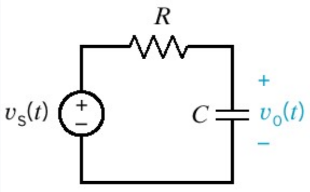
\includegraphics[width=.9\linewidth]{./images/rc-circuit-diagram.png}
\end{center}

The square signal exciting the RC circuit:
\begin{center}
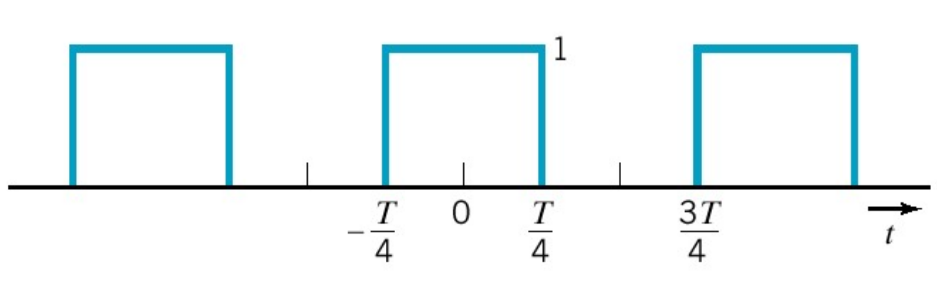
\includegraphics[width=.9\linewidth]{./images/even-square-wave-function.png}
\end{center}

 \newpage
\subsubsection{Equivalent circuit}
\label{sec:org554f93c}
In the equivalent circuit below, each voltage source is a term of the Fourier series of the input voltage \(v_s (t)\).
\begin{center}
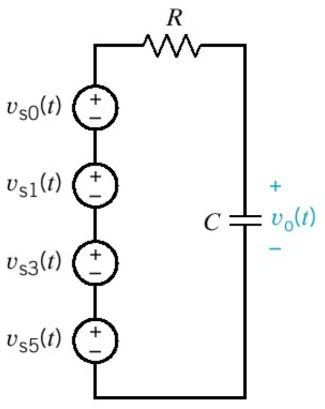
\includegraphics[height=18em]{./images/rc-equivalent-circuit-diagram.png}
\end{center}
\subsubsection{Steady state response of the circuit}
\label{sec:orgaa68990}
Since each input is a sinusoid, we want to find the steady state responses to the sinusoid.
\begin{center}
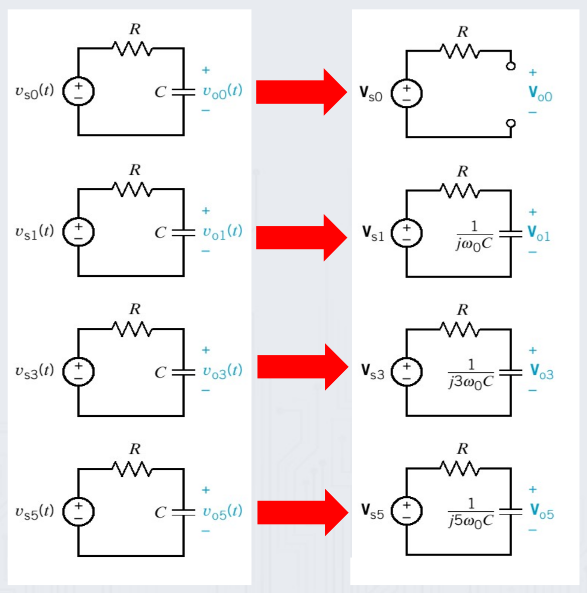
\includegraphics[height=18em]{./images/rc-circuit-steady-state-response.png}
\end{center}
\subsubsection{Making use of the Fourier series}
\label{sec:orgd55fb33}
The Fourier series representation of the square waveform:
\[F(t) = \frac{1}{2} + \frac{2}{\pi} \cos \left(1 \cdot \frac{2 \pi}{T} \cdot t \right) - \frac{2}{3 \pi} \cos \left( 3 \cdot \frac{2 \pi}{T} \cdot t \right) + \frac{2}{5 \pi} \cos \left( 5 \cdot \frac{2 \pi}{T} \cdot t \right) - \frac{2}{7 \pi} \cos \left( 7 \cdot \frac{2 \pi}{T} \cdot t \right) + \ldots\]

Since \(T = \pi\), the first 4 terms of \(v_s (t)\) are:
\[v_s(t) \approx \underbrace{\frac{1}{2}}_{v_{s0} (t)} + \underbrace{\frac{2}{\pi} \cos 2t}_{v_{s1} (t)} - \underbrace{\frac{2}{3 \pi} \cos 6t}_{v_{s3 (t)}} + \underbrace{\frac{2}{5 \pi} \cos 10t}_{v_{s5} (t)}\]

The steady state response \(v_0 (t)\) can be found using superposition:
\[v_o (t) = v_{o0} (t) + v_{o1} (t) + v_{o3} (t) + v_{o5} (t)\]
\subsubsection{Getting the impedance of the capacitor}
\label{sec:org745965f}
The impedance of the capacitor is:
\[Z_c = \frac{1}{jn \omega_0 C}, \text{ for } n = 0, 1, 3, 5, \ldots\]

Because:
\[T = \pi, \quad \omega_0 = \frac{2 \pi}{T} = \qty{2}{\sec}\]

Since:
\[R = \qty{1}{\ohm}, \quad C = \qty{2}{F}, \quad T = \pi \ \unit{\sec}\]

We can find:
\begin{align*}
V_{on} &= \frac{\frac{1}{jn \omega_0 C}}{R + \frac{1}{jn \omega_0 C}} V_{sn} \\
&= \frac{V_{sn}}{1 + jn \omega_0 CR} \\
&= \frac{V_{sn}}{1 + j4n} \\
&= \frac{(1 - j4n) V_{sn}}{(1 - j4n)(1 + j4n)} \\
&= \frac{(1 - j4n) V_{sn}}{(1 + 16n^2)} \\
&= \frac{1}{\sqrt{1 + 16n^2}} \left(\frac{1}{\sqrt{1 + 16n^2}} - j \frac{4n}{\sqrt{1 + 16n^2}} \right) V_{sn}
\end{align*}

Let \(\theta_n = - \arctan (4n)\):
\begin{align*}
V_{on} &= \frac{1}{\sqrt{1 + 16n^2}} (\cos \theta_n + j \sin \theta_n) V_{sn} \\
&= \frac{1}{\sqrt{1 + 16n^2}} e^{i \theta n} V_{sn}, \quad n = 0, 1, 3, 5, \ldots
\end{align*}

Since \(V_{sn} = |V_{sn}| e^{jn \omega_0 t} = \frac{2}{n \pi} e^{i2nt}\):
\begin{align*}
V_{on} &= \frac{1}{\sqrt{1 + 16n^2}} e^{i \theta n} V_{sn} \\
&= \frac{2}{n \pi \sqrt{1 + 16n^2}} e^{2nt + \theta_n}
\end{align*}

When \(n = 0\):
\[V_{o0} = \frac{1}{2}\]

When \(n = 1\):
\[\theta_1 = - \arctan (4 \times 1) = \qty{-75.96}{\degree}\]
\[V_{o1} = \frac{2}{1 \pi \sqrt{1 + 16 \times 1^2}} e^{i 2 \times 1t (-75.96)} = 0.1544e^{i(2t - \qty{75.96}{\degree})}\]

When \(n = 3\):
\[\theta_3 = - \arctan (4 \times 3) = \qty{-85.24}{\degree}\]
\[V_{o3} = \frac{2}{3 \pi \sqrt{1 + 16 \times 3^2}} e^{i 2 \times 3t (-85.24)} = 0.0176e^{i(6t - \qty{85.24}{\degree})}\]

When \(n = 5\):
\[\theta_5 = - \arctan (4 \times 5) = \qty{-87.14}{\degree}\]
\[V_{o5} = \frac{2}{5 \pi \sqrt{1 + 16 \times 5^2}} e^{i 2 \times 5t (-87.14)} = 0.0063e^{i(10t - \qty{87.14}{\degree})}\]

Therefore:
\[v_o (t) = 0.5 + 0.1544 \cos (2t - \qty{75.96}{\degree}) + 0.0176 \cos (6t - \qty{85.24}{\degree}) + 0.0063 \cos (10t - \qty{87.14}{\degree})\]

 \newpage
\subsection{Conditions for the Fourier series}
\label{sec:org6b82332}
To be described by the Fourier series, the waveform \(f(t)\) must satisfy the following mathematical properties:
\begin{itemize}
\item \(f(t)\) is a \textbf{single-value} function, except at possibly a finite number of points.
\item For any \(t_0\), the integral \(\int_{t_0}^{t_0 + T} |f(t)| \, dt < \infty\).
\item \(f(t))\) has a finite number of \textbf{discontinuities} within the period \(T\).
\item \(f(t)\) has a finite number of \textbf{maxima} and \textbf{minima} within the period \(T\).
\end{itemize}

In practice, \(f(t)\) is usually an amplitude function, so the above 4 conditions are always satisfied.
\subsection{Insights}
\label{sec:org469fdf2}

\subsubsection{Frequency response methods}
\label{sec:orgefef4ee}
Giving a different kind of insight into a system with insights of unexpected results.
\subsubsection{Frequency spectrum}
\label{sec:org129b969}
Focusing on how signals of different frequencies are represented in a signal thus with insights in terms of the spectrum of the signal.
\subsubsection{Computer processing}
\label{sec:org6827980}
Often, it is easier and more cost-effective to characterise the frequency content of a noise signal than to give a time description of the noise.
\subsubsection{Applications}
\label{sec:org7f400b4}
Different treatment of different parts of the electromagnetic spectrum means that you can separate the different radio, television and cell phone signals.

 \newpage
\section{Bandwidth and frequency response}
\label{sec:org1906fd8}
\begin{itemize}
\item It is important to estimate the spectrum of a signal when choosing a \textbf{measurement} system.
\item Ideal \textbf{measurement} systems replicates all frequency components of an input signal.
\item Practical \textbf{measurement} systems have limitations in reproducing all frequencies.
\end{itemize}
\subsection{Decibel scale}
\label{sec:org6744878}
The common scale used to \textbf{measure} fidelity of a measurement system's reproduction at different frequencies is the decibel scale:
\[dB = 20 \log_{10} \left(\frac{A_{out}}{A_{in}} \right)\]

Where:
\begin{itemize}
\item \(A_{in}\) is the input amplitude of a harmonic
\item \(A_{out}\) is the output amplitude of a harmonic
\end{itemize}
\subsection{Frequency response curve (Bode plot)}
\label{sec:orgcb26f1c}
A frequency response curve or a Bode plot plots \(\frac{A_{out}}{A_{in}}\) versus input frequency.

\begin{center}
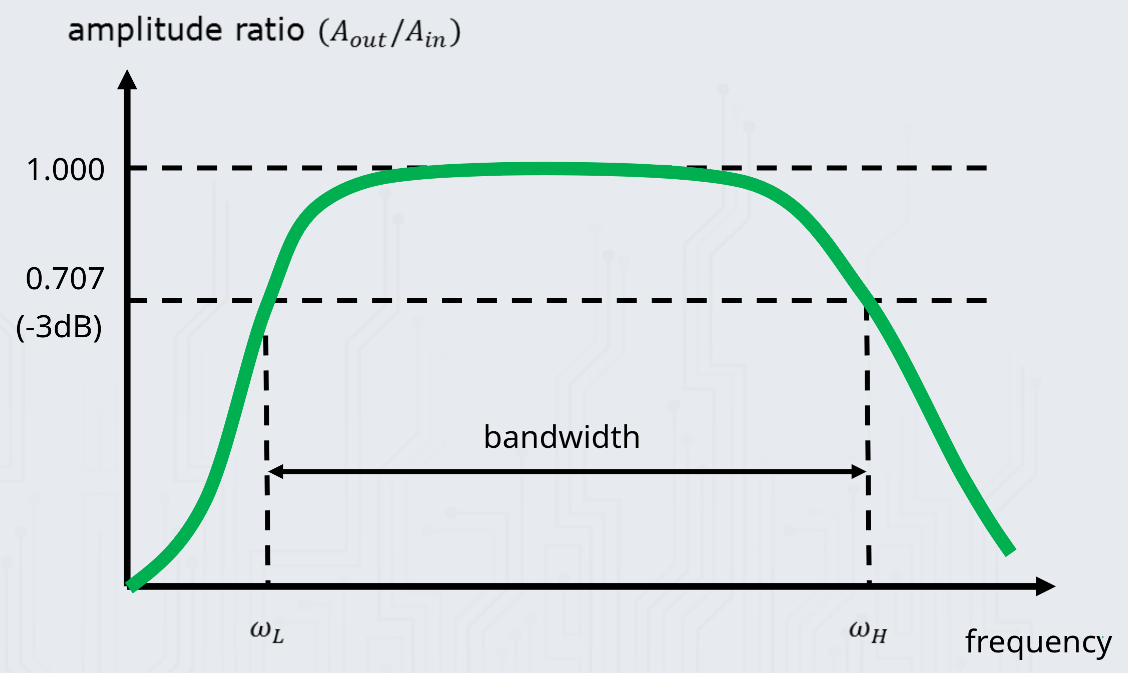
\includegraphics[width=.9\linewidth]{./images/frequency-response-curve.png}
\end{center}
\subsection{Bandwidth}
\label{sec:orga4b8445}
Bandwidth is the range of the frequencies where the input is not attenuated, i.e. the amplitude is not reduced, or the volume is not reduced, by more than \(\qty{-3}{\dB}\), i.e.
\[\text{Bandwidth} = \omega_L \text{ to } \omega_h\]

Where:
\begin{itemize}
\item \(\omega_L\) is the low cut-off or corner frequency
\item \(\omega_L\) is the high cut-off or corner frequency
\end{itemize}

 \newpage
\subsubsection{Why \(\qty{-3}{dB}\)?}
\label{sec:org98dc32c}
The value comes from half of the output power over the input power, i.e.

\begin{align*}
\frac{1}{2} &= \frac{P_{out}}{P_{in}} = \left(\frac{A_{out}}{A_{in}} \right)^2 \\
& \Rightarrow \frac{A_{out}}{A_{in}} = \sqrt{\frac{1}{2}} \\
& \Rightarrow \unit{dB} = 20 \log_{10} \sqrt{\frac{1}{2}} \\
& \approx \qty{-3}{dB}
\end{align*}
\subsubsection{Example}
\label{sec:org010cad0}
Calculating output amplitude \(A'_i\) given a \textbf{measurement} frequency response curve, with the input signal spectrum as:
\[V_{in} (t) = A_1 \sin (\omega_0 t) + A_2 \sin (2 \omega_0 t) + A_3 \sin (3 \omega_0 t) + \cdots\]

\begin{center}
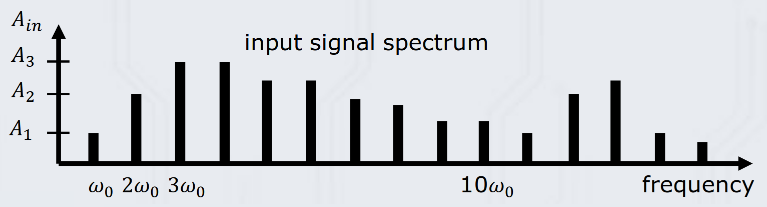
\includegraphics[width=.9\linewidth]{./images/bandwidth-example-input-signal-spectrum.png}
\end{center}

The output amplitude \(A'_i\) is calculated as:
\[A'_i = \left( \frac{A_{out}}{A_{in}} \right) A_i\]

\begin{center}
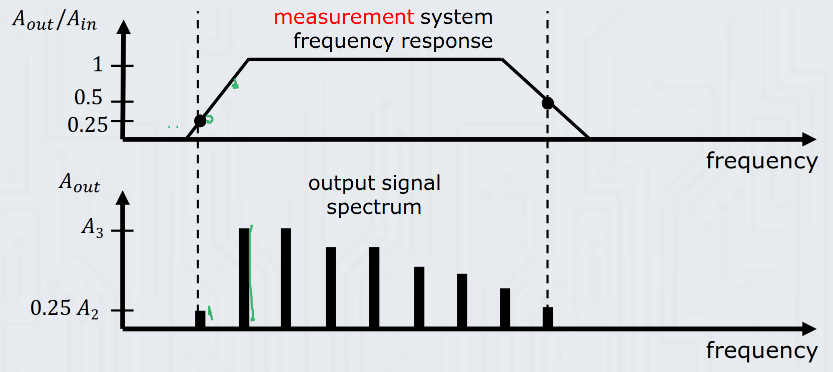
\includegraphics[width=.9\linewidth]{./images/bandwidth-example-measurement-system-frequency-response-and-output-signal-spectrum.png}
\end{center}
\section{Periodic functions}
\label{sec:orgd944641}

\subsection{Definition}
\label{sec:orgebf2b8a}
A periodic function is any function of time that satisfies the following:
\[f(t + T) = f(t)\]

Where:
\begin{itemize}
\item \(T\) is a constant called the \textbf{period} of the function
\end{itemize}
\subsection{Even-function symmetry}
\label{sec:orge778842}
Any function of time \(f(t)\) that satisfies the below condition is called an \textbf{even function}.
\[f(-t) = f(t)\]

\begin{center}
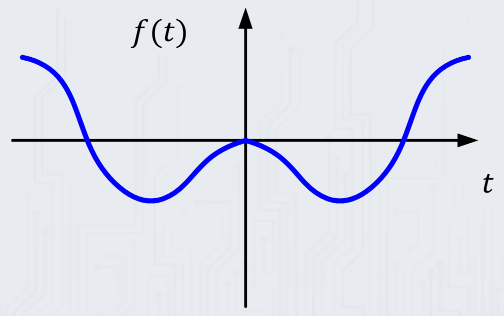
\includegraphics[width=.9\linewidth]{./images/even-function-symmetry.png}
\end{center}

 \newpage
\subsection{Odd-function symmetry}
\label{sec:orgff04d59}
Any function of time \(f(t)\) that satisfies the below condition is called an \textbf{odd function}.
\[f(-t) = - f(t)\]

\begin{center}
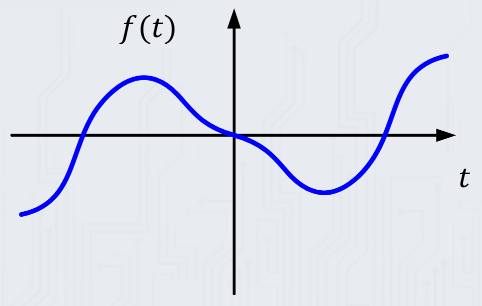
\includegraphics[width=.9\linewidth]{./images/odd-function-symmetry.png}
\end{center}
\subsection{Properties of symmetric functions}
\label{sec:org6d27757}
Let \(f(t)\) be a periodic function with period \(T\).

\begin{center}
\begin{tabular}{l|l}
\(f(t)\) & \(\int_{-\frac{T}{2}}^{\frac{T}{2}} f(t) \, dt\)\\
\hline
Even & \(\int_{-\frac{T}{2}}^{\frac{T}{2}} f(t) \, dt = 2 \int_0^{\frac{T}{2}} f(t) \, dt\)\\
Odd & \(\int_{-\frac{T}{2}}^{\frac{T}{2}} f(t) \, dt = 0\)\\
\end{tabular}
\end{center}
\subsection{Conversion from non-periodic to periodic}
\label{sec:org1cc05c3}

\subsubsection{Original pattern}
\label{sec:org3678c69}
\begin{center}
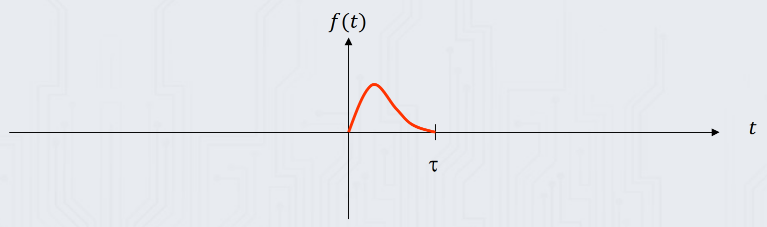
\includegraphics[width=.9\linewidth]{./images/original-pattern.png}
\end{center}
A non-periodic function \(f(t)\) defined over \((0, t)\) can be expanded into a Fourier series which is defined only in the interval \((0, t)\). Note that the original pattern may not necessarily pass the origin.
\subsubsection{Without considering symmetry}
\label{sec:orge39b1e7}
\begin{center}
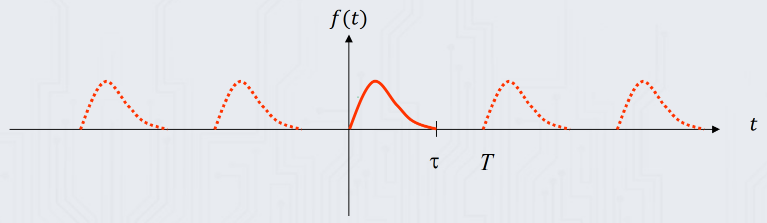
\includegraphics[width=.9\linewidth]{./images/non-symmetric-repeated-pattern.png}
\end{center}
One simple technique that can be applied is to offset the original pattern along the time axis by a distance of \(nT (\tau < T), n = \pm 1, \pm 2, \pm 3, \ldots\)

 \newpage
\subsubsection{Expansion into even-function symmetry}
\label{sec:org627caca}
\begin{center}
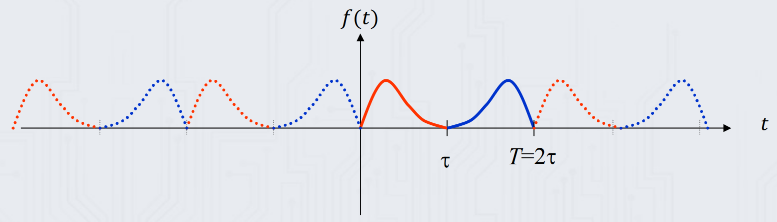
\includegraphics[width=.9\linewidth]{./images/even-function-symmetry-repeated-pattern.png}
\end{center}
A second pattern can be created by mirroring the original pattern against an axis \(t = \tau\).

An even-function symmetric periodic waveform can be generated by offsetting the two patterns merged along the time axis by a distance \(nT (T = 2 \tau), n = \pm 1, \pm 2, \pm 3, \ldots\)
\subsubsection{Expansion into odd-function symmetry}
\label{sec:org7f83d68}
\begin{center}
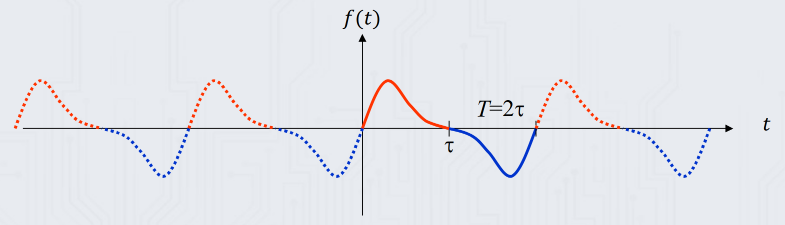
\includegraphics[width=.9\linewidth]{./images/odd-function-symmetry-repeated-pattern.png}
\end{center}
A third pattern can be created by mirroring the original pattern against the time axis and then the axis \(t = \tau\).

An odd-function periodic waveform can be generated by offsetting the two patterns merged along the time axis by a distance \(nT (T = 2 \tau), n = \pm 1, \pm 2, \pm 3, \ldots\)
\subsection{Examples}
\label{sec:org4531f5f}

\subsubsection{Square signal}
\label{sec:org2a8fb23}
\begin{center}
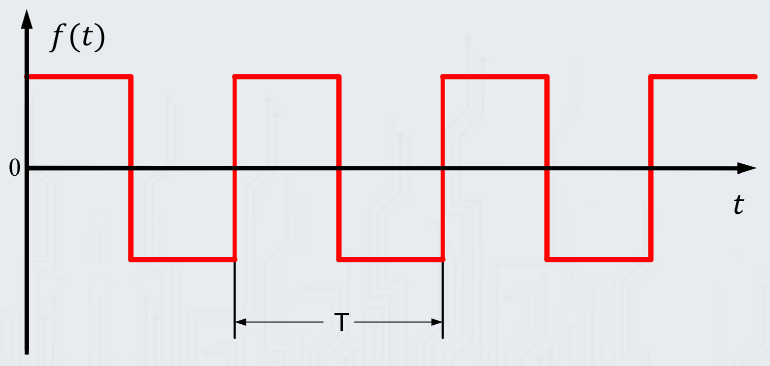
\includegraphics[width=.9\linewidth]{./images/square-signal.png}
\end{center}
\subsubsection{Triangular signal}
\label{sec:orgbc54661}
\begin{center}
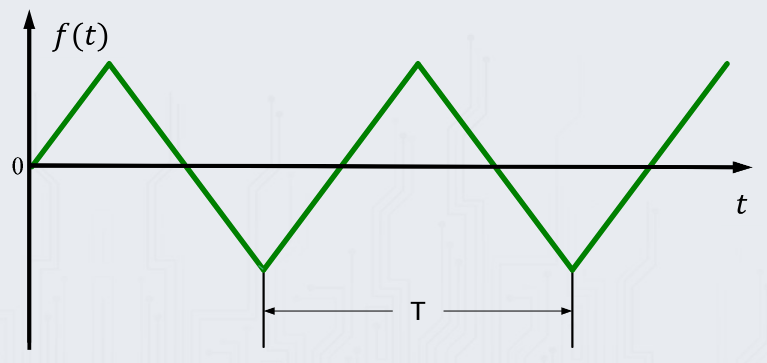
\includegraphics[width=.9\linewidth]{./images/trianglular-signal.png}
\end{center}
\subsubsection{Sawtooth signal}
\label{sec:org20ae222}
\begin{center}
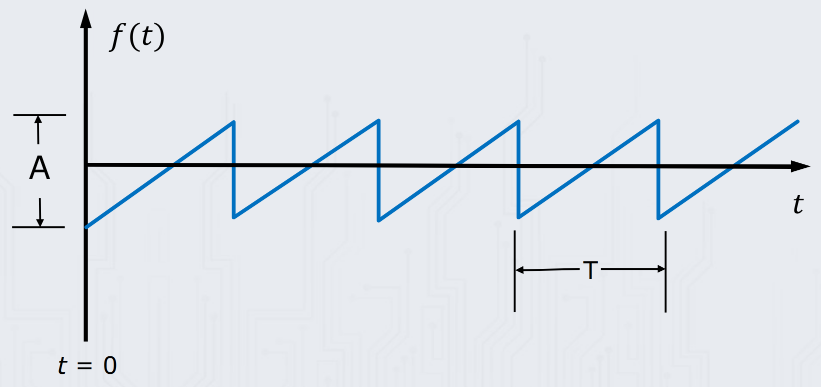
\includegraphics[width=.9\linewidth]{./images/sawtooth-signal.png}
\end{center}
\subsubsection{Pulse signal}
\label{sec:orgde6d19f}
\begin{center}
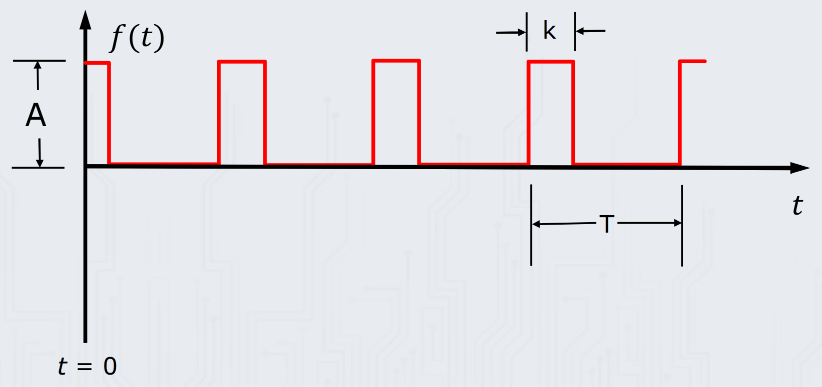
\includegraphics[width=.9\linewidth]{./images/pulse-signal.png}
\end{center}
\subsubsection{Rectified signal}
\label{sec:org9922dc4}
\begin{center}
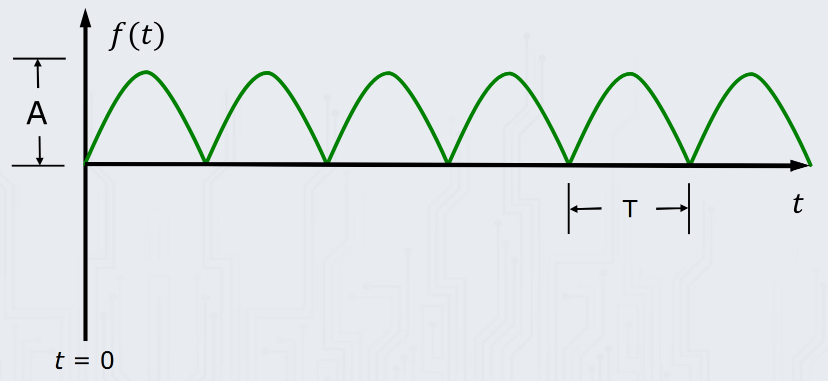
\includegraphics[width=.9\linewidth]{./images/rectified-signal.png}
\end{center}
\subsubsection{General periodic signal}
\label{sec:orgc7f7d73}
\begin{center}
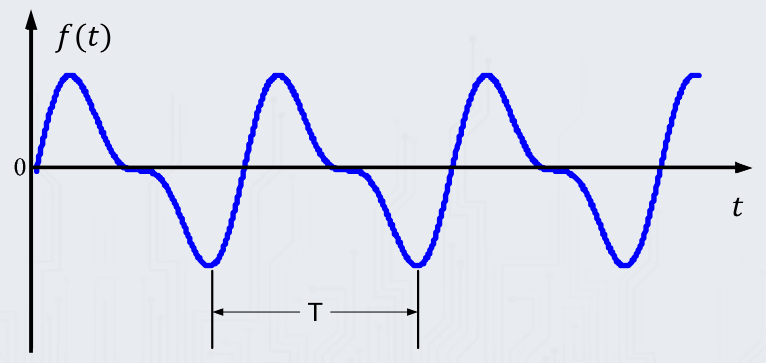
\includegraphics[width=.9\linewidth]{./images/general-periodic-signal.png}
\end{center}

 \newpage
\section{Dynamic systems}
\label{sec:org27f3c9e}

\subsection{Example 1}
\label{sec:org599138f}
A linear potentiometer used as a position sensor.
\begin{center}
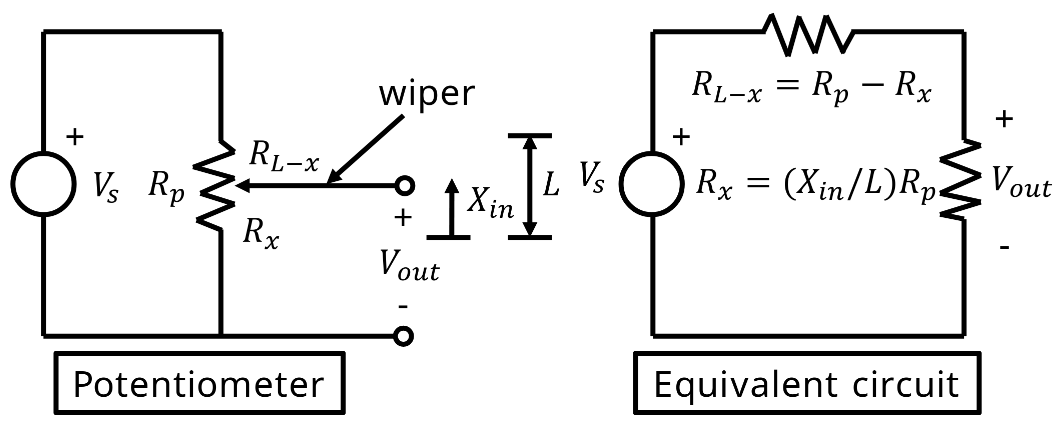
\includegraphics[width=.9\linewidth]{./images/linear-potentiometer-used-as-position-sensor.png}
\end{center}

The system behaviour is:
\[V_{out} = \frac{R_x}{R_p} V_s = \frac{V_s}{L} X_{in}\]

Where:
\begin{itemize}
\item \(X_{in}\) is the wiper displacement with the potentiometer
\item \(R_p\) is the maximum resistance of the potentiometer
\item \(R_x\) is the resistance between the potentiometer leads
\item \(L\) is the maximum amount of wiper travel
\end{itemize}

 \newpage
\subsection{Example 2}
\label{sec:orge08e3fe}
A resistor-capacitor circuit.
\begin{center}
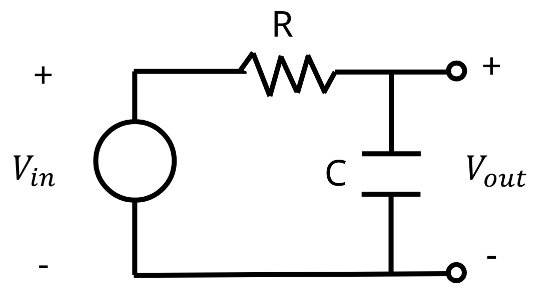
\includegraphics[width=.9\linewidth]{./images/resistor-capacitor-circuit.png}
\end{center}

In this system, applying Kirchhoff's Laws and the voltage-current relations for a resistor and capacitor produces a first order linear differential equation relating the output voltage to the input voltage.

The system behaviour is:
\[RC = \frac{dV_{out}}{dt} + V_{out} = V_{in}\]

Where:
\begin{itemize}
\item \(R\) is the resistance of the resistor
\item \(C\) is the capacitance of the capacitor
\item \(V_{out}\) is the output voltage
\item \(V_{in}\) is the input voltage
\end{itemize}

 \newpage
\subsection{Example 3 (second-order system)}
\label{sec:orgee7c7e4}
A spring damping system.
\begin{center}
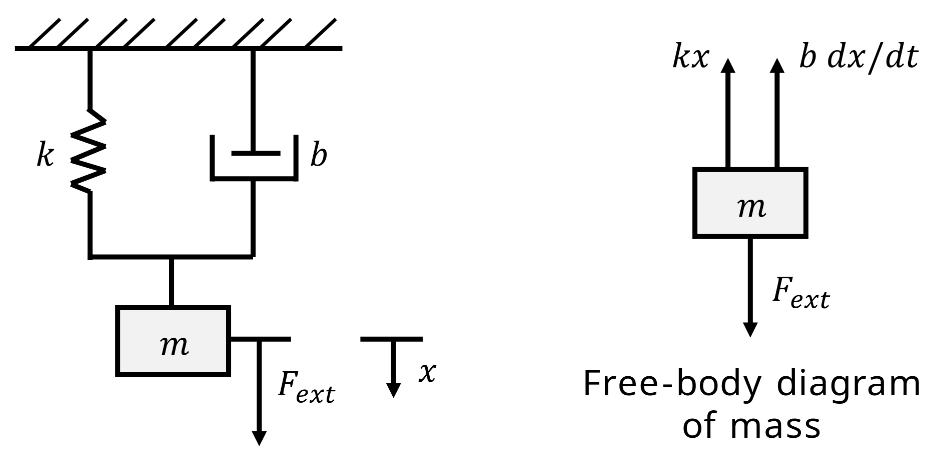
\includegraphics[width=.9\linewidth]{./images/spring-damping-system.png}
\end{center}

The system behaviour is:
\[m \frac{d^2 x}{dt^2} + b \frac{dx}{dt} + kx = F_{ext} (t)\]

Where:
\begin{itemize}
\item \(m\) is the mass of the block
\item \(b\) is the damping coefficient
\item \(k\) is the spring constant
\item \(x\) is the displacement of the mass from the equilibrium (rest) position of the mass
\item \(F_{ext} (t)\) is the external force along the \(x\)-direction
\end{itemize}
\subsection{Measurement system: Ordinary differential equations}
\label{sec:orge5724ad}
\begin{center}
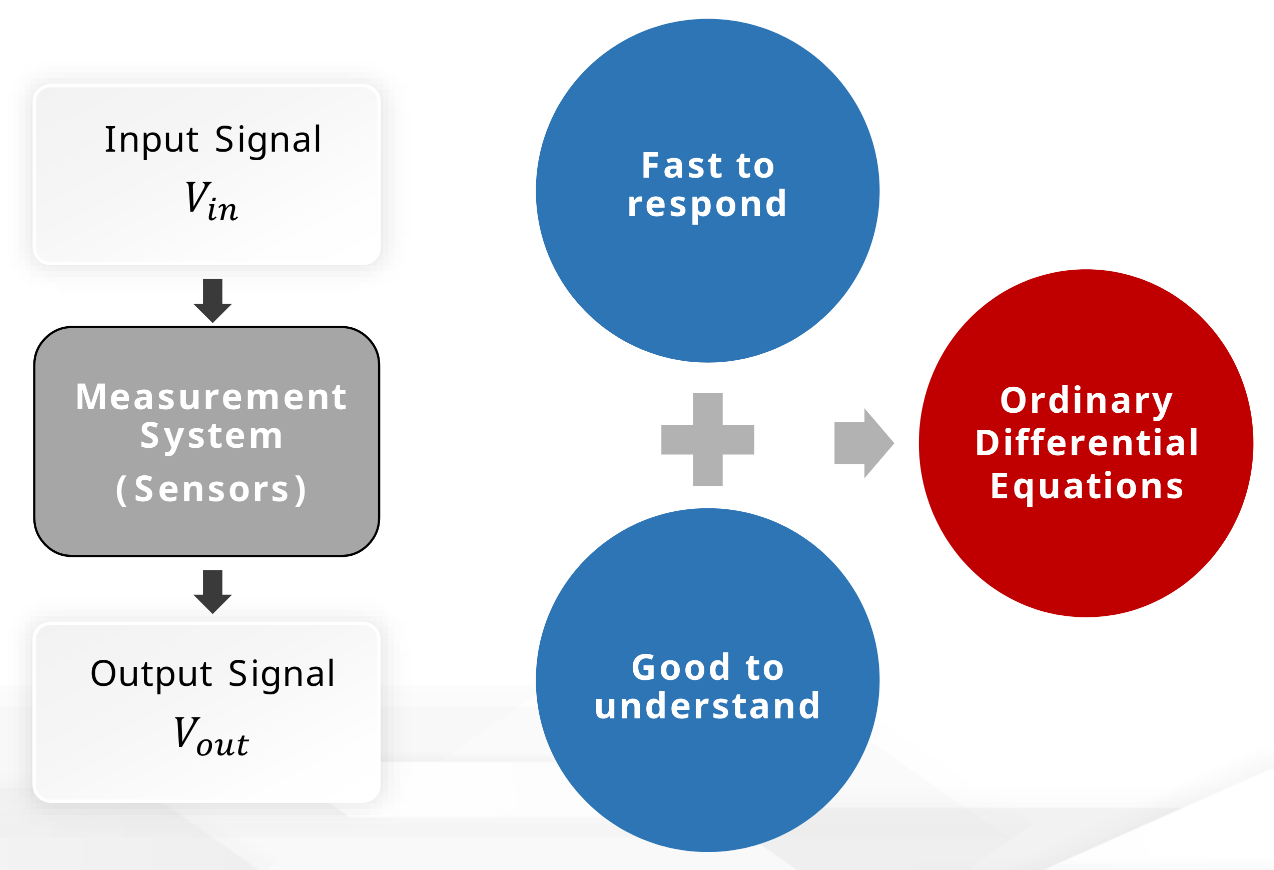
\includegraphics[width=.9\linewidth]{./images/dynamic-systems-measurement-system.png}
\end{center}
\subsubsection{Why ordinary differential equations?}
\label{sec:org005d275}
\begin{itemize}
\item Ordinary differential equations have time as the only variable.
\item Ordinary differential equations can be used to explain the behaviour of a dynamic system.
\item At steady state, there is no change, which means there is no need to use ordinary differential equations in steady state.
\end{itemize}

 \newpage
\section{Linear systems}
\label{sec:org3c6de48}
\begin{itemize}
\item Linear systems are of the form:
\begin{align*}
&A_n \frac{d^N X_{out}}{dt^N} + A_{N - 1} \frac{d^{N - 1} X_{out}}{dt^{N - 1}} + \cdots A_1 \frac{d X_{out}}{dt} + A_0 X_{out} \\
&= B_M \frac{d^M X_{in}}{dt^M} + B_{M - 1} \frac{d^{M - 1} X_{in}}{dt^{M - 1}} + \cdots + B_1 \frac{dX_{in}}{dt} + B_0 X_{in}
\end{align*}
\item Alternatively:
\[\sum_{n = 0}^N A_n \frac{d^n X_{out}}{dt^n} = \sum_{m = 0}^M B_m \frac{d^m X_{in}}{dt^m}\]
\item The word "linear" comes from the coefficients:
\[A_n (n = 0, \ldots, N) \text{ and } B_m (m = 0, \ldots, M)\]
\end{itemize}

Where:
\begin{itemize}
\item \(X_{in}\) and \(X_{out}\) are input and output variables
\item \(A_n\) and \(B_m\) are coefficients
\item \(N\) is the order of the system
\end{itemize}
\subsection{Homogeneous equation of a linear system}
\label{sec:org1ebbf16}
\[\sum_{n = 0}^N A_n \frac{d^n X_{out}}{dt^n} = 0\]

Where:
\begin{itemize}
\item \(X_{out}\) is the output variables
\item \(A_n\) is a coefficient
\item \(N\) is the order of the system
\end{itemize}
\subsection{Characteristic equation of a homogeneous equation}
\label{sec:org025264c}
\[\sum_{n = 0}^N A_n s^n = 0\]

Where:
\begin{itemize}
\item \(A_n\) and \(s\) are coefficients
\item \(N\) is the order of the system
\end{itemize}
\subsubsection{Primary (\(N = 1\))}
\label{sec:org0e0f95a}
\[A_1 s + A_0 = 0\]
\[s = \frac{A_0}{A_1}, \text{ if } A_0 \ne 0\]
\subsubsection{Quadratic (\(N = 2\))}
\label{sec:orga0d66d0}
\[A_2 s^2 + A_1 s + A_0 = 0\]
\[s = \frac{- A_1 \pm \sqrt{A_1^2 - 4 A_0 A_2}}{2 A_2}, \text{ if } A_2 \ne 0\]
\subsection{Roots of the characteristic equation}
\label{sec:orgfb1688c}
\[\sum_{n = 0}^N A_n s^n = 0, A_N \ne 0\]
\subsubsection{When \(N = 1\)}
\label{sec:orgae356ec}
Single real root:
\[s_1 = r\]

Where:
\begin{itemize}
\item \(s_1\) is the coefficient of the characteristic equation
\item \(r\) is the root
\end{itemize}
\subsubsection{When \(N = 2\)}
\label{sec:org61663ac}
\begin{itemize}
\item Double real roots:
\[s_1 = s_2 = r\]
\item Two different real roots:
\[s_1 \ne s_2\]
\item Two conjugate roots:
\[s_1 = a + bi, \quad s_2 = a - bi\]
\end{itemize}
\subsubsection{When \(N = k\)}
\label{sec:orgc58010a}
Multiple k-fold real roots:
\[s_1 = \ldots = s_k = r\]
\subsection{Solving the homogeneous equation}
\label{sec:org6bdaab7}

\subsubsection{When \(N = 1\)}
\label{sec:orgb275070}
\begin{itemize}
\item Single real root: \(s_1 = r\)
\item General solution for the homogeneous equation:
\[C_0 e^{rt}\]
\end{itemize}
\subsubsection{When \(N = 2\)}
\label{sec:org675e713}
\begin{enumerate}
\item Two conjugate roots:
\[s_1 = a + bi, \quad s_2 = a - bi\]

General solution for the homogeneous equation:
\[(C_1 \sin (bt) + C_2 \cos (bt)) e^{at}\]

\item Two different real roots:
\[s_1 \ne s_2\]

General solution for the homogeneous equation:
\[C_1 e^{s_1 t} + C_2 e^{s_2 t}\]

\item Double real roots:
\[s_1 = s_2 = r\]

General solution for the homogeneous equation:
\[(C_1 + C_2 t) e^{rt}\]
\end{enumerate}
\subsubsection{When \(N = k\)}
\label{sec:orgb18885c}
\begin{itemize}
\item Multiple k-fold real roots:
\[s_1 = s_2 = \ldots = s_k = r\]
\item General solution for the homogeneous equation:
\[(C_0 + C_1 t + C_2 t^2 + \ldots + C_{k - 1} t^{k - 1}) e^{rt}\]
\end{itemize}
\subsection{Input functions in a linear system}
\label{sec:org8e3b873}
\begin{itemize}
\item Step input
\item Sinusoidal input
\item Pulse input
\item Square input
\end{itemize}
\subsection{Special cases of linear systems}
\label{sec:org2d25373}

\subsubsection{Zero-order system}
\label{sec:org7ed8786}
\begin{itemize}
\item \(M = 0\)
\item \(N = 0\)
\end{itemize}

\[A_0 X_{out} = B_0 X_{in}\]

Where:
\begin{itemize}
\item \(A_0\) and \(B_0\) are coefficients
\item \(X_{out}\) and \(X_{in}\) are output and input variables
\end{itemize}
\subsubsection{First-order system}
\label{sec:org491f0cf}
\begin{itemize}
\item \(M = 0\)
\item \(N = 1\)
\end{itemize}

\[A_1 \frac{dX_{out}}{dt} + A_0 X_{out} = B_0 X_{in}\]

Where:
\begin{itemize}
\item \(A_1\), \(A_0\) and \(B_0\) are coefficients
\item \(X_{out}\) and \(X_{in}\) are output and input variables
\end{itemize}
\subsubsection{Second-order system}
\label{sec:org9bacc7a}
\begin{itemize}
\item \(M = 0\)
\item \(N = 2\)
\end{itemize}

\[A_2 \frac{d^2 X_{out}}{dt^2} + A_1 \frac{d X_{out}}{dt} + A_0 X_{out} = B_0 X_{in}\]

Where:
\begin{itemize}
\item \(A_1\), \(A_2\), \(A_0\) and \(B_0\) are coefficients
\item \(X_{out}\) and \(X_{in}\) are output and input variables
\end{itemize}
\subsection{Zero-order system}
\label{sec:org1b36582}

\subsubsection{Example}
\label{sec:orgf4e428e}
\begin{center}
\includegraphics[width=.9\linewidth]{./images/linear-potentiometer-used-as-position-sensor.png}
\end{center}

Where:
\begin{itemize}
\item \(X_{in}\) is the wiper displacement with the potentiometer
\item \(R_p\) is the maximum resistance of the potentiometer
\item \(R_x\) is the resistance between the potentiometer leads
\item \(L\) is the maximum amount of wiper travel
\end{itemize}

System behaviour:
\[V_{out} = \frac{R_x}{R_p} V_s = \frac{V_s}{L} X_{in}\]

Zero-order system:
\[A_0 X_{out} = B_0 X_{in}\]
\subsubsection{General zero-order system}
\label{sec:org016501b}
\[A_0 X_{out} = B_0 X_{in}\]
\[X_{out} = \frac{B_0}{A_0} X_{in}\]
\[X_{out} = K X_{in}\]

Where:
\begin{itemize}
\item \(X_{out}\) and \(X_{in}\) are output and input variables
\item \(K\) is a constant called \textbf{gain} or \textbf{sensitivity}
\end{itemize}
\subsubsection{Remarks}
\label{sec:org5427cf1}
A zero-order system follows the input exactly without any time delay or distortion.
\[\text{Input Signal } X_{in} \rightarrow \text{Degenerated differential equations} \rightarrow \text{Output signal } X_{out}\]

The input signals can be of any periodic waveform.
\subsection{First-order system}
\label{sec:org7dee199}

\subsubsection{Example}
\label{sec:orga42213f}
\begin{center}
\includegraphics[height=15em]{./images/resistor-capacitor-circuit.png}
\end{center}

In this system, applying Kirchhoff's Laws and the voltage-current relations for a resistor and capacitor produces a first order linear differential equation relating the output voltage to the input voltage.

System behaviour:
\[RC = \frac{dV_{out}}{dt} + V_{out} = V_{in}\]
\subsubsection{General first-order system}
\label{sec:org5be93dc}
When \(N = 1\) and \(M = 0\):
\begin{align*}
&A_1 \frac{dX_{out}}{dt} + A_0 X_{out} = B_0 X_{in} \\
&\rightarrow \tau \frac{dX_{out}}{dt} + X_{out} \\
&= KX_{in}
\end{align*}

Where:
\begin{itemize}
\item \(K = \frac{B_0}{A_0}\) is the static sensitivity
\item \(\tau = \frac{A_1}{A_0}\) is the time constant
\end{itemize}

Hence, the first-order system equation can be written as:
\[\tau \frac{dX_{out}}{dt} + X_{out} = KX_{in}\]

Note that in this standard form, the coefficient of the \(X_{out}\) term must be 1, hence:
\[A_0 \ne 0\]
\subsubsection{Step response of first-order systems}
\label{sec:orgb56b2e6}
The step input changes instantaneously from 0 to a constant value \(A_{in}\) and is stated mathematically as:
\begin{align*}
X_{in} = \begin{cases}
0 & t < 0 \\
A_{in} & t \ge 0
\end{cases}
\end{align*}

The output of the system in response to this input is called the step response of the system. For a first-order system, we can find the step response by solving the first-order ordinary differential equation below:
\[\tau \frac{dX_{out}}{dt} + X_{out} = KX_{in}\]

Initial condition:
\[X_{out} (0) = 0\]

Characteristic equation:
\[\tau s + 1 = 0\]

Roots of the characteristic equation:
\[s = - \frac{1}{\tau}\]
\subsubsection{Solving the homogeneous equation}
\label{sec:orgc5ffcfd}
\begin{itemize}
\item Linear system:
\[\tau \frac{dX_{out}}{dt} + X_{out} = KX_{in}\]
\item Homogeneous equation:
\[\tau s + 1 = 0\]
\item Root:
\[r = - \frac{1}{\tau}\]
\item General solution for the homogeneous equation:
\[X_{out_h} = C_0 e^{- \frac{t}{\tau}}\]

Where:
\begin{itemize}
\item \(C_0\) is a constant determined later by applying initial conditions
\end{itemize}

\item A particular or steady state solution resulting form the step input \(X_{in} = A_{in}\):
\[X_{out_p} = KA_{in}\]
\item General solutions for the linear system:
\[X_{out} = X_{out_h} + X_{out_p} = C_0 e^{- \frac{t}{\tau}} + KA_{in}\]
\end{itemize}
\subsubsection{Determining the step response of the first-order system}
\label{sec:orgbcc0269}
Determining the constant by initial conditions:
\[\tau \frac{dX_{out}}{dt} + X_{out} = KX_{in}\]
\[X_{out} = X_{out_h} + X_{out_p} = C e^{- \frac{t}{\tau}} + KA_{in}\]

Applying the initial condition \(\left.X_{out} \right|_{t = 0} = X_{out} (0)\) to this equation gives:
\[X_{out} (0) = C + KA_{in}\]

Thus:
\[C = X_{out} (0) - KA_{in}\]

So, the resulting step response is:
\[X_{out} = X_{out} (0) e^{- \frac{t}{\tau}} + KA_{in} (1 - e^{- \frac{t}{\tau}})\]

If \(X_{out} (0) = 0\):
\[X_{out} = KA_{in} (1 - e^{- \frac{t}{\tau}})\]
\subsubsection{Graph of the step response of the first-order system}
\label{sec:orgd7a32bf}
\begin{align*}
&\tau \frac{dX_{out}}{dt} + X_{out} = KX_{in} \\
&\rightarrow X_{out} = KA_{in} (1 - e^{- \frac{t}{\tau}})
\end{align*}
\begin{align*}
&X_{out} = X_{out_h} + X_{out_p} = C e^{- \frac{t}{\tau}} + KA_{in} \\
&\rightarrow X_{out} (0) = 0
\end{align*}

\begin{center}
\includegraphics[width=.9\linewidth]{./images/step-response-of-first-order-system-graph.png}
\end{center}

\begin{itemize}
\item The graph above represents an exponential rise in the output toward an asymptotic value of \(KA_{in}\).
\item The rate of rise depends only on the time constant \(\tau\).
\item The response is faster for a smaller time constant.
\item After one time constant, the output reaches 63.2\% of its final value:
\[X_{out} (t = \tau) = KA_{in} (1 - e^{- \frac{t}{\tau}} = 0.632 KA_{in})\]
\item After four time constants, the step response is:
\[X_{out} (t = 4 \tau) = KA_{in} (1 - e^{- \frac{4t}{\tau}}) = 0.982 KA_{in}\]
\item Since this value is more than 98\% of the steady state value \(KA_{in}\), we usually assume that a first-order system has reached its steady state value within four time constants.
\item When designing a first-order measurement system, look at quantities that affect \(\tau\) and try to reduce them if possible.
\item The larger \(\tau\) is, the longer the measurement system takes to respond to an input.
\end{itemize}
\subsection{Second-order system}
\label{sec:org5a33388}
\[A_2 \frac{d^2 X_{out}}{dt^2} + A_1 \frac{dX_{out}}{dt} + A_0 X_{out} = B_0 X_{in}\]
\subsubsection{Example}
\label{sec:org4378f76}
\begin{center}
\includegraphics[width=.9\linewidth]{./images/spring-damping-system.png}
\end{center}

Where:
\begin{itemize}
\item \(m\) is the mass of the block
\item \(b\) is the damping coefficient
\item \(k\) is the spring constant
\item \(x\) is the displacement of the mass from the equilibrium (rest) position of the mass
\item \(F_{ext} (t)\) is the external force along the \(x\)-direction
\end{itemize}

System behaviour:
\[m \frac{d^2 x}{dt^2} + b \frac{dx}{dt} + kx = F_{ext} (t)\]

 \newpage
\subsubsection{Equations}
\label{sec:orgaea66e6}
\begin{itemize}
\item \(M = 0, N = 2\)
\item Homogeneous equation:
\[A_2 \frac{d^2 X_{out}}{dt^2} + A_1 \frac{dX_{out}}{dt} + A_0 X_{out} = 0\]
\item Characteristic equation:
\[A_2 s^2 + A_1 s + A_0, \quad A_2 \ne 0\]
\item Roots of the characteristic equation:
\[A_2 s^2 A_1 s + A_0 = 0, \quad A_2 \ne 0\]
\[s = \frac{- A_1 \pm \sqrt{A_1^2 - 4 A_0 A_2}}{2 A_2}, \text{ if } A_2 \ne 0\]
\end{itemize}

 \newpage
\subsubsection{Solving the homogeneous equation}
\label{sec:org4bbc914}
\begin{itemize}
\item Homogeneous equation:
\[\sum_{n = 0}^N A_n \frac{d^n X_{out}}{dt^n} = 0\]
\item Characteristic equation:
\[\sum_{n = 0}^N A_n s^n = 0, \quad A_N \ne 0\]
\item Two conjugate roots:
\[s_1 = a + bi, \quad s_2 = a - bi\]

General solution for the homogeneous equation:
\[(C_1 \sin (bt) + C_2 \cos (bt)) e^{at}\]

\item Two different real roots:
\[s_1 \ne s_2\]

General solution for the homogeneous equation:
\[C_1 e^{s_1 t} + C_2 e^{s_2 t}\]

\item Double real roots:
\[s_1 = s_2 = r\]

General solution for the homogeneous equation:
\[(C_1 + C_2 t) e^{rt}\]
\end{itemize}

 \newpage
\subsubsection{Unforced response of a second-order system}
\label{sec:orgdee7188}
\[m \frac{d^2 x}{dt^2} + b \frac{dx}{dt} + kx = 0\]

Characteristic equation of the second-order system:
\[ms^2 + bs + k = 0\]

Roots of the characteristic equation:
\[s_1 = - \frac{b}{2m} + \sqrt{\left(\frac{b}{2m} \right)^2 - \frac{k}{m}}\]
\[s_2 = - \frac{b}{2m} - \sqrt{\left(\frac{b}{2m} \right)^2 - \frac{k}{m}}\]
\subsubsection{Unforced response without damping, with \(b = 0\)}
\label{sec:orgd124a6a}
\[m \frac{d^2 x}{dt^2} + b \frac{dx}{dt} + kx = 0, \quad ms^2 + k = 0\]

Roots of the second order system:
\[s_1 = i \sqrt{k}{m}, \quad s_2 = - i \sqrt{k}{m}\]

Homogeneous solution:
\[x_h (t) = A \cos \left(\sqrt{\frac{k}{m}} \right) + B \sin \left(\sqrt{\frac{k}{m}} t \right)\]

Coefficients \(A\) and \(B\) could be determined by the initial conditions:
\[x(t = 0), \quad \left. \frac{dx (t)}{dx} \right|_{t = 0}\]

Natural frequency of undamped oscillatory motion with radian frequency:
\[\omega_n = \sqrt{\frac{k}{m}}\]

Under this frequency, the undamped system would naturally oscillate if the spring were stretched and the mass is released and allowed to move without any external force (\(F_{ext} = 0\))
\subsubsection{Unforced response without damping, with \(b \ne 0\)}
\label{sec:org0e35e22}
\[m \frac{d^2 x}{dt^2} + b \frac{dx}{dt} + kx = 0, \quad ms^2 + bs + k = 0\]

If the \(\text{Radicand} = 0\), the roots of the second-order system are:
\[\text{Radicand} = \sqrt{b^2 - 4mk} = 0 \rightarrow b^2 = 4mk\]
\[s_1 = s_2 = - \frac{b}{2m} = - \sqrt{\frac{4mk}{4m^2}} = - \sqrt{\frac{k}{m}}\]

Homogeneous solution:
\[x_h (t) = (A + Bt) e^{- \omega_n t} A = \pi r \omega_n^2 = \sqrt{\frac{k}{m}}\]

Coefficients \(A\) and \(B\) could be determined by the initial conditions:
\[x (t = 0), \quad \left. \frac{dx (t)}{dt} \right|_{x = 0}\]

Solution:
\[x_h (t) = (A + Bt) e^{- \omega_n t}\]

This represents an exponential decaying motion.

For critical damping, if the \(\text{radicand} = 0\), the critical damping constant is:
\[b_c = 2 \sqrt{mk} = 2m \sqrt{\frac{k}{m}} = 2 m \omega_n\]

For non-critical damping, if the \(\text{radicand} \ne 0\), the damping ratio is:
\[\zeta = \frac{b}{b_c} = \frac{b}{2 \sqrt{mk}}\]

Note:
\begin{enumerate}
\item Damping ratio is a measure of the proximity to critical damping.
\item A critically damped system has a damping ratio of 1.
\end{enumerate}
\subsubsection{Properties}
\label{sec:orge85865e}
\begin{itemize}
\item Homogeneous equation:
\[m \frac{d^2 x}{dt^2} + b \frac{dx}{dt} + kx = 0\]
\item Characteristic equation:
\[ms^2 + bs + k = 0\]
\item Roots of the second-order system
\[s = \frac{-b \pm \sqrt{b^2 - 4mk}}{2m}\]

Because:
\[b_c = 2 \sqrt{mk} = 2m \sqrt{\frac{k}{m}} = 2 m \omega_n\]
\[\zeta = \frac{b}{b_c} = \frac{b}{2 \sqrt{mk}}\]

\item 2 different real roots of the second-order system:
\begin{align*}
s &= \frac{-b \pm \sqrt{b^2 - 4mk}}{2m} \\
&= \frac{- \frac{b}{b_c} \pm \sqrt{\frac{b^2}{b_c^2}} - \frac{4mk}{b_c^2}}{2 \cdot \frac{m}{b_c}} \\
&= \frac{- \zeta \pm \sqrt{\zeta^2 - 1}}{\frac{1}{\omega_n}} \\
&= -\zeta \omega_n \pm \omega_n \sqrt{\zeta^2 - 1}
\end{align*}

Where:
\begin{itemize}
\item \(\zeta\) is the damping ratio
\item \(\omega_n\) is the natural frequency
\end{itemize}
\end{itemize}
\subsubsection{Under damped system (\(\zeta < 1\), with 2 complex conjugate roots)}
\label{sec:org77f3311}
\begin{itemize}
\item Roots
\[s_1 = - \zeta_{\omega_n} + j \omega_n \sqrt{1 - \zeta^2}\]
\[s_2 = - \zeta_{\omega_n} - j \omega_n \sqrt{1 - \zeta^2}\]
\item Homogeneous solution:
\[x_h(t) = e^{-\zeta \omega_n t} \left[A \cos \left(\omega_n \sqrt{1 - \zeta^2 t} \right) + B \sin \left(\omega_n \sqrt{1 - \zeta^2 t} \right) \right]\]
\item This motion represents damped oscillation consisting of sinusoidal motion with exponentially decaying amplitude.
\[\omega_d = \omega_n \sqrt{1 - \zeta^2}\]
\item The frequency of oscillation is called the damped natural frequency.
\end{itemize}
\subsubsection{Overdamped system (\(\zeta > 1\), with 2 real roots)}
\label{sec:orgfa81578}
\begin{itemize}
\item Roots:
\[s_1 = -\zeta \omega_n + \omega_n + \sqrt{\zeta^2 - 1}\]
\[s_2 = -\zeta \omega_n - \omega_n + \sqrt{\zeta^2 - 1}\]
\item Homogeneous solution:
\[x_h (t) = Ae^{\left(- \zeta + \sqrt{\zeta^2 - 1} \right) \omega_n t} + Be^{\left( -\zeta - \sqrt{- \zeta^2 - 1} \right) \omega_n t}\]
\item This motion represents an exponential decaying output.
\end{itemize}

 \newpage
\subsubsection{Graphs of unforced responses}
\label{sec:org1004c4c}
With initial conditions:
\[x(0) = 1, \quad \left. \frac{dx (t)}{dt} \right|_{t = 0} = 0\]

\begin{center}
\includegraphics[width=.9\linewidth]{./images/graph-of-unforced-responses.png}
\end{center}

 \newpage
\subsubsection{Summary}
\label{sec:orgfc00ca3}
Let's define:
\[\text{Natural frequency, } \omega_n = \sqrt{\frac{k}{m}}\]
\[\text{Damping ratio, } \zeta = \frac{b}{2 \sqrt{km}}\]

We have:
\[m \frac{d^2 x}{dt^2} + b \frac{dx}{dt} + kx = 0\]
\[\frac{d^2 x}{dt^2} + 2 \zeta \omega_n \frac{dx}{dt} + \omega_n^2 x = 0\]

The characteristic equation is:
\[s^2 + 2 \zeta \omega_n s + \omega_n^2 = 0\]

Whose roots are:
\[s_1 = -\zeta \omega_n + \omega_n + \sqrt{\zeta^2 - 1}\]
\[s_2 = -\zeta \omega_n - \omega_n + \sqrt{\zeta^2 - 1}\]

As \(F_{ext} = 0\) (unforced).  \\

When \(\zeta = 0\) (undamped):
\[x_h (t) = a \cos (\omega_n t) + B \sin(\omega_n t)\]

When \(\zeta < 1\) (under damped):
\[x_h(t) = e^{-\zeta \omega_n t} \left[A \cos \left(\omega_n \sqrt{1 - \zeta^2 t} \right) + B \sin \left(\omega_n \sqrt{1 - \zeta^2 t} \right) \right]\]

When \(\zeta > 1\) (overdamped):
\[x_h (t) = Ae^{\left(- \zeta + \sqrt{\zeta^2 - 1} \right) \omega_n t} + Be^{\left( -\zeta - \sqrt{- \zeta^2 - 1} \right) \omega_n t}\]

Where the coefficients \(A\) and \(B\) are determined from the initial conditions.
\subsubsection{Forced response of a second-order system}
\label{sec:orgcae68b2}
A second-order system will have forced response when \(F_{ext} (t) \ne 0\). For the second-order system:
\[m \frac{d^2 x}{dt^2} + b \frac{dx}{dt} + kx = F_{ext} (t)\]

Its solution can be obtained by combining a general solution (\(x_h (t)\)) of its homogeneous equation, and a particular solution (\(x_p (t)\)) of the second-order system.
\[x(t) = x_h (t) + x_p (t)\]

When the external force has step input:
\begin{displaymath}
F_{ext} = \begin{cases}
0 & t < 0 \\
F_i & t \ge 0
\end{cases}
\end{displaymath}

\begin{center}
\includegraphics[width=.9\linewidth]{./images/forced-response-step-input-graph.png}
\end{center}

It is easy to see that the second-order system \(m \frac{d^2 x}{dt^2} + b \frac{dx}{dt} + kx = F_{ext} (t)\) has a particular solution:
\[x_p (t) = \frac{F_i}{k}\]

Because:
\[\frac{k F_i}{k} = F_i\]
\subsubsection{Solving the homogeneous equation of the forced response of a second-order system}
\label{sec:orged8ce38}
The homogeneous equation can be solved using the same technique developed for the unforced response of the second-order system.  \\

As \(F_{ext} = 0\) (unforced response).  \\

When \(\zeta = 0\) (undamped):
\[x_h (t) = A \cos(\omega_n t) + B \sin(\omega_n t)\]

When \(\zeta = 1\) (critically damped):
\[x_h (t) = (A + Bt) e^{- \omega_n t}\]

When \(\zeta < 1\) (under damped):
\[x_h(t) = e^{-\zeta \omega_n t} \left[A \cos \left(\omega_n \sqrt{1 - \zeta^2 t} \right) + B \sin \left(\omega_n \sqrt{1 - \zeta^2 t} \right) \right]\]

When \(\zeta > 1\) (overdamped):
\[x_h (t) = Ae^{\left(- \zeta + \sqrt{\zeta^2 - 1} \right) \omega_n t} + Be^{\left( -\zeta - \sqrt{- \zeta^2 - 1} \right) \omega_n t}\]
\subsubsection{Graphs of forced responses}
\label{sec:orge935cff}
\begin{center}
\includegraphics[width=.9\linewidth]{./images/forced-response-damping-graph.png}
\end{center}

Initial conditions:
\[x (t = 0) = 0, \quad \left. \frac{dx(t)}{dt} \right|_{t = 0} = 0\]
\subsubsection{Characteristics of a graph of forced response}
\label{sec:orgd904d6e}
\begin{center}
\includegraphics[width=.9\linewidth]{./images/forced-response-graph-characteristics.png}
\end{center}

Where:
\begin{itemize}
\item "Steady state value" refers to the value where the system reaches after all transients have dissipated.
\item "Rise time" refers to the time required for the system to go form 10\% to 90\% of the steady state value.
\item "Over-shoot" is a measure of the amount the output exceeds the steady state value.
\item "Settling time" refers to the time required for the system to settle to within an amplitude band whose width is a specific \(\pm 10\%\) of the steady state value.
\end{itemize}
\subsubsection{Forced response amplitude ratio vs frequency ratio graph}
\label{sec:orgce4d1b9}
\begin{center}
\includegraphics[width=.9\linewidth]{./images/forced-response-amplitude-vs-frequency-graph.png}
\end{center}

Note that \(\zeta = \frac{1}{\sqrt{2}} \approx 0.707\) provides the best amplitude linearity over the largest bandwidth.
\section{System modelling and analogies}
\label{sec:org1a24024}

\subsection{System models}
\label{sec:org079404c}
\begin{center}
\includegraphics[width=.9\linewidth]{./images/system-models.png}
\end{center}

The systems on the right-hand side of the image are the system that are analogous to the models on the left-hand side.

 \newpage
\subsection{Second-order modelling analogies}
\label{sec:org65970c1}
\begin{center}
\begin{tabularx}{1.2\textwidth}{| >{\centering\arraybackslash}X| >{\centering\arraybackslash}X| >{\centering\arraybackslash}X| >{\centering\arraybackslash}X| >{\centering\arraybackslash}X|}
\hline
Generic quantity & Mechanical translation & Mechanical rotation & Electrical & Hydraulic\\
\hline
Effort (\(E\)) & Force (\(F\)) & Torque (\(T\)) & Voltage (\(V\)) & Pressure (\(P\))\\
\hline
Flow (\(F\)) & Speed (\(v\)) & Angular speed (\(\omega\)) & Current (\(i\)) & Volumetric flow rate (\(Q\))\\
\hline
Displacement (\(q\)) & Displacement (\(x\)) & Angular displacement (\(\theta\)) & Charge (\(q\)) & Volume (\(V\))\\
\hline
Momentum (\(p\)) & Linear momentum (\(p = mv\)) & Angular momentum (\(h = J \omega\)) & Flux linkage (\(I = N \Phi = Li\)) & \(\frac{\text{Momentum}}{\text{Area}}\) (\(\Gamma = IQ\))\\
\hline
Resistor (\(R\)) & Damper (\(b\)) & Rotatory damper (\(B\)) & Resistor (\(R\)) & Resistor (\(R\))\\
\hline
Capacitor (\(C\)) & Spring \(\left(\frac{1}{k} \right)\) & Torsion spring \(\left(\frac{1}{k} \right)\) & Capacitor (\(C\)) & Tank (\(C\))\\
\hline
Inertia (\(I\)) & Mass (\(m\)) & Moment of inertia (\(J\)) & Inductor (\(L\)) & Inertance (\(I\))\\
\hline
Inertia energy storage (special case) & \(F = \dot{p}\) (\(F = ma\)) & \(T = \dot{h}\) (\(T = J \alpha\)) & \(V = \dot{\lambda}\) \(\left(V = L \frac{di}{dt} \right)\) & \(P = \dot{\Gamma}\) \(\left(P = I \frac{dQ}{dt} \right)\)\\
\hline
Capacitor energy storage & \(F = kx\) & \(T = k \theta\) & \(V = \frac{1}{C} q\) & \(P = \frac{1}{C} V\)\\
\hline
Dissipative & \(F = bv\) & \(T = B \omega\) & \(V = Ri\) & \(P = RQ\)\\
\hline
\end{tabularx}
\end{center}

 \newpage
\subsection{Similarities and differences}
\label{sec:org83904a7}

\subsubsection{Similarities}
\label{sec:org6516db4}
\begin{itemize}
\item Mathematical representation
\item Mathematical solution
\item Mathematical properties
\end{itemize}
\subsubsection{Differences}
\label{sec:orga4e8f30}
\begin{itemize}
\item Constants (coefficients, or parameters)
\item Physical meanings of these parameters of the system
\end{itemize}
\subsubsection{Analogies}
\label{sec:orgad7b3b7}
\begin{itemize}
\item For those parameters among the different system types: Resistors, valves, mass, inertia, \ldots{}
\item System terms: Effort, flow, displacement, momentum, resistance, capacitance, \ldots{}
\end{itemize}
\section{Sampling}
\label{sec:org04ba19a}

\subsection{Sampling rate}
\label{sec:org6175b5e}
\begin{itemize}
\item Higher sampling rates allow the waveform to be more accurately represented.
\item Low sampling rates may lead the waveform to be less accurately represented.
\end{itemize}

\begin{center}
\includegraphics[width=.9\linewidth]{./images/sampling-rate-comparison-graphs.png}
\end{center}
\subsection{Analogue vs digital signals}
\label{sec:org0ecee8c}
\begin{center}
\begin{tabular}{l|l}
Analogue signal & Digital signal\\
\hline
Continuous & Discrete\\
Generated via analogue devices & Sampled in a fixed interval\\
Not coded & Coded value\\
Original signal & Sequential data array\\
\end{tabular}
\end{center}
\subsection{Shannon \& Nyquist theorem}
\label{sec:org3e8aeed}
The best explanation for the Shannon \& Nyquist sampling theorem is \href{https://www.youtube.com/watch?v=Jv5FU8oUWEY}{this YouTube video}.
\subsubsection{Sampling \(\qty{1}{Hz}\) sine wave at \(\qty{2}{Hz}\)}
\label{sec:org0cd6c8c}
\begin{center}
\includegraphics[width=.9\linewidth]{./images/sampling-1hz-sine-wave-at-2hz.png}
\end{center}

There are sufficient samples to capture each peak and trough of the signal.
\subsubsection{Sampling \(\qty{1}{Hz}\) sine wave at \(\qty{3}{Hz}\)}
\label{sec:orgb8a2a56}
\begin{center}
\includegraphics[width=.9\linewidth]{./images/sampling-1hz-sine-wave-at-3hz.png}
\end{center}

There are more than enough samples to capture the variations in the signal.

 \newpage
\subsubsection{Sampling \(\qty{1}{Hz}\) sine wave at \(\qty{1.5}{Hz}\)}
\label{sec:orgb211fe2}
\begin{center}
\includegraphics[width=.9\linewidth]{./images/sampling-1hz-sine-wave-at-1.5hz.png}
\end{center}

There isn't enough samples to capture all the peaks and troughs in the signal, which results in information being lost.

The signal may also be misinterpreted as a \(\qty{0.5}{Hz}\) signal, as shown below:
\begin{center}
\includegraphics[width=.9\linewidth]{./images/sampling-0.5hz-sine-wave.png}
\end{center}
\subsection{Why don't we sample as fast as possible?}
\label{sec:orgedb3ff0}
\begin{itemize}
\item Sampling as fast as possible results in huge amounts of data.
\item It also requires high speed software.
\item A lot of storage is needed to store the data.
\end{itemize}
\subsection{Logic behind the minimum sampling rate}
\label{sec:org5902d56}
\begin{itemize}
\item We need to sample a digital signal at a rate more than 2 times the \textbf{maximum frequency} \((f_{max})\) \textbf{component} in the signal to retain all frequency components.
\item To faithfully represent the analogue signal, the digital samples must be taken at a frequency \(f_s\), such that:
\[f_s > 2 f_{max}\]

Where:
\begin{itemize}
\item \(f_s\) is the \textbf{sampling rate} (not sampling frequency)
\item \(f_{max}\) is the maximum frequency in the signal, also known as the \textbf{Nyquist frequency}
\end{itemize}

\item If we approximate a signal by a truncated Fourier series (\(N\) terms), the maximum frequency component is the \textbf{highest harmonic frequency}. Hence, the time interval between the digital samples is:
\[\Delta t = \frac{1}{f_s}\]
\end{itemize}
\subsection{Theorem}
\label{sec:orgb877f28}
\[F(t) = \sum_{n = 0}^N C_n \cos (n \omega_0 t + \phi_n)\]
\[f(t) = \sum_{n = -N}^{N} D_n e^{jn \omega_0 t}\]

Where:
\begin{itemize}
\item \(N\) is the maximum frequency component of the signal
\item \(f_s\) is the sampling rate
\item \(f_{max}\) is the Nyquist frequency
\end{itemize}
\subsubsection{Shannon-Nyquist Theorem}
\label{sec:org3bcc8e0}
\[f_s > 2f_{max}\]

Where:
\begin{itemize}
\item \(f_s\) is the sampling rate
\item \(f_{max}\) is the Nyquist frequency
\end{itemize}
\subsubsection{Time interval between the digital samples (\(\Delta t\))}
\label{sec:org41d8989}
\[\Delta t = \frac{1}{f_s}\]

Where:
\begin{itemize}
\item \(\Delta t\) is the time interval between the digital samples
\item \(f_s\) is the sampling rate
\end{itemize}
\subsubsection{Sampling \(\qty{1}{Hz}\) sine wave at \(\qty{2}{Hz}\)}
\label{sec:org871a238}
\begin{center}
\includegraphics[width=.9\linewidth]{./images/sampling-1hz-sine-wave-at-2hz.png}
\end{center}

\begin{itemize}
\item Maximum frequency component: \(N = 1\)
\item Nyquist frequency: \(f_{max} = \qty{1}{Hz}\)
\item Sampling rate: \(f_s = \qty{2}{Hz}\)
\item Time interval between digital samples: \(\Delta t = \frac{1}{2} \ \unit{sec}\)
\end{itemize}
\subsubsection{Sampling \(\qty{1}{Hz}\) sine wave at \(\qty{1.5}{Hz}\)}
\label{sec:org9e75fc3}
\begin{center}
\includegraphics[width=.9\linewidth]{./images/sampling-1hz-sine-wave-at-1.5hz.png}
\end{center}

\begin{itemize}
\item Maximum frequency component: \(N = 1\)
\item Nyquist frequency: \(f_{max} = \qty{1}{Hz}\)
\item Sampling rate: \(f_s = \qty{1.5}{Hz}\)
\item Time interval between digital samples: \(\Delta t = \frac{1}{1.5} = \frac{2}{3} \ \unit{sec}\)
\end{itemize}
\subsubsection{Sampling a sine wave with multiple frequencies at \(\qty{6}{Hz}\)}
\label{sec:org62dcb3b}
\begin{center}
\includegraphics[width=.9\linewidth]{./images/sampling-sine-wave-with-muliple-frequencies-at-6hz.png}
\end{center}

\begin{itemize}
\item Maximum frequency component: \(N = 3\)
\item Nyquist frequency: \(f_{max} = \qty{3}{Hz}\)
\item Sampling rate: \(f_s = \qty{6}{Hz}\)
\item Time interval between digital samples: \(\Delta t = \frac{1}{6} \ \unit{sec}\)
\end{itemize}
\subsection{Aliasing}
\label{sec:org33dd418}

\subsubsection{Sampling of a clock with only one hand}
\label{sec:org8beb9df}
\begin{itemize}
\item Sampling a clock at double the Nyquist frequency:
\begin{center}
\includegraphics[width=.9\linewidth]{./images/sampling-clock-at-double-nyquist-frequency.png}
\end{center}

\begin{itemize}
\item Sampling rate: \(f_s = \frac{1}{30} \ \unit{Hz}\)
\item Nyquist frequency: \(f_{max} = \frac{1}{60} \ \unit{Hz}\)
\item Double Nyquist frequency: \(f_{max} = \frac{1}{30} \ \unit{Hz}\)
\item Aliasing occurs as the receiver cannot tell if the clock is moving forward or backwards.
\end{itemize}

\item Sampling of a clock above double the Nyquist frequency:
\begin{center}
\includegraphics[width=.9\linewidth]{./images/sampling-clock-above-double-nyquist-frequency.png}
\end{center}

\begin{itemize}
\item Sampling rate: \(f_s = \frac{1}{15} \ \unit{Hz}\)
\item Nyquist frequency: \(f_{max} = \frac{1}{60} \ \unit{Hz}\)
\item Double Nyquist frequency: \(f_{max} = \frac{1}{30} \ \unit{Hz}\)
\item No aliasing occurs as the receiver can tell that the clock is moving forward.
\end{itemize}
\end{itemize}

 \newpage

\begin{itemize}
\item Sampling of a clock under double the Nyquist frequency:
\begin{center}
\includegraphics[width=.9\linewidth]{./images/sampling-clock-under-double-nyquist-frequency.png}
\end{center}

\begin{itemize}
\item Sampling rate: \(f_s = \frac{1}{45} \ \unit{Hz}\)
\item Nyquist frequency: \(f_{max} = \frac{1}{60} \ \unit{Hz}\)
\item Double Nyquist frequency: \(f_{max} = \frac{1}{30} \ \unit{Hz}\)
\item Aliasing occurs as the receiver thinks that the clock is moving backwards instead of forward.
\end{itemize}
\end{itemize}

 \newpage
\subsubsection{Undersampled signal}
\label{sec:org79a959e}
Below is a signal with a frequency of \(\qty{8}{Hz}\) sampled at a rate of \(\qty{8.5}{Hz}\)
\begin{center}
\includegraphics[width=.9\linewidth]{./images/sampling-undersampled-signal.png}
\end{center}

An undersampled signal can confuse you about its frequency when reconstructed as the sampling rate is too low.
\subsubsection{Reconstruction of a sampled sine wave}
\label{sec:org90268c3}
\begin{center}
\includegraphics[width=.9\linewidth]{./images/sampling-reconstruction-of-sampled-sine-wave.png}
\end{center}
\subsubsection{Frequency of aliased signal (\(f_a\))}
\label{sec:org1a167ce}
The frequency of an aliased signal (\(f_a\)) is given as:
\[f_a = \left|f_s \cdot i - f_n \right|\]

Where:
\begin{itemize}
\item \(f_a\) is the frequency of the aliased signal
\item \(f_s\) is the sampling rate
\item \(i\) is the closest integer multiple of the sampling rate to the signal being aliased
\item \(f_n\) is the frequency of the signal being aliased
\end{itemize}

For example, if the signal is \(f_n = \qty{21}{Hz}\) and is sampled with \(f_s = \qty{10}{Hz}\), then the aliased frequency would be \(\left| i \cdot f_s - f_n \right| = | 2 \cdot 10 - 21 | = \qty{1}{Hz}\)
\subsubsection{Capturing the shape of the waveform}
\label{sec:org89f35e3}
Even though sampling at twice the \textbf{Nyquist frequency} will ensure that you measure the correct frequency of your signal, it will not be sufficient to capture the shape of the waveform.

If the shape of the waveform is desired, you should sample at a rate approximately \textbf{10 times} the \textbf{Nyquist frequency}.
\subsection{Applications}
\label{sec:org95bb8c8}

\subsubsection{Recording audio}
\label{sec:orgd25bdcf}
\begin{itemize}
\item The range of human hearing is \(20 - 20,000 \ \unit{Hz}\).
\item We lose high frequency response with age.
\item Women generally have better response than men.
\item To reproduce an audio signal of \(\qty{20}{kHz}\) requires a sampling rate of at least \(\qty{40}{kHz}\).
\item \textbf{Below} the sampling rate of \(\qty{40}{kHz}\), aliasing will occur, according the Shannon-Nyquist Theorem.
\end{itemize}
\subsubsection{Digital voice telephone transmission}
\label{sec:org263b7ce}
\begin{itemize}
\item Voice data for telephone purposes is limited to frequencies less than \(\qty{4}{kHz}\).
\item According to the Shannon-Nyquist Theorem, it would take 8,000 samples \(2 \cdot 4,000\) to capture a \(4,000 \ \unit{Hz}\) signal perfectly.
\item Generally, one byte is recorded per sample (256 levels). One byte is eight bits of binary data.
\item \(\qty{8}{bits} \cdot 8,000 \text{ samples per second } = \qty{64}{kbps}\) over a circuit.
\end{itemize}

 \newpage
\section{Quantisation and encoding}
\label{sec:org01f6972}

\subsection{Digitising}
\label{sec:orgd2aa66f}
\begin{center}
\includegraphics[width=.9\linewidth]{./images/digitising-sound.png}
\end{center}

\begin{center}
\includegraphics[width=.9\linewidth]{./images/playing-back-the-digital-sound-file.png}
\end{center}
\subsection{Pulse code modulation (PCM)}
\label{sec:orgb2f41a3}
\begin{itemize}
\item Pulse code modulation consists of three steps to digitise an analogue signal:
\begin{enumerate}
\item Sampling
\item Quantisation
\item Binary encoding
\end{enumerate}
\item Before we sample, we have to filter the signal to limit the maximum frequency of the signal as it affects the sampling rate.
\item Filtering should ensure that we do not distort the signal by removing high frequency components that affect the signal shape.
\end{itemize}
\subsubsection{Components of a PCM encoder}
\label{sec:orga84b659}
\begin{center}
\includegraphics[width=.9\linewidth]{./images/components-of-a-pcm-encoder.png}
\end{center}
\subsubsection{Sampling methods and pulse amplitude modulation (PAM)}
\label{sec:org60e48fc}
\begin{itemize}
\item The analogue signal is sampled every \(T_s \ \unit{secs}\).
\item \(T_s\) is known as the sampling interval.
\item \(f_s = \frac{1}{T_s}\) is called the sampling rate or sampling frequency.
\item There are 3 sampling methods:
\begin{enumerate}
\item Ideal, which is an instant pulse at each sampling instant.
\item Natural, which is a pulse of short width with varying amplitude.
\item Flat top, which is to sample and hold the value. It is similar to the natural sampling method, but with a constant amplitude value.
\end{enumerate}
\item This process is known as pulse amplitude modulation (PAM) and the outcome is a signal with analogue (non-integer) values.
\end{itemize}
\subsubsection{Images of the sampling methods}
\label{sec:org14b2ec3}
\begin{center}
\includegraphics[height=15em]{./images/ideal-sampling.png}
\end{center}

\begin{center}
\includegraphics[height=15em]{./images/natural-sampling.png}
\end{center}

\begin{center}
\includegraphics[height=15em]{./images/flat-top-sampling.png}
\end{center}
\subsection{Quantisation}
\label{sec:org59db49f}
\begin{itemize}
\item Sampling results in a series of pulses of varying amplitude values ranging between two limits: a minimum and a maximum value.
\item The amplitude values are finite between the two limits.
\item We need to map the finite amplitude values onto a finite set of known values.
\item This is achieved by dividing the distance between the minimum and maximum into \(L\) zones, each of height \(\Delta\)
\[\Delta = \frac{max - min}{L}\]
\end{itemize}

 \newpage
\subsubsection{Analogue quantisation size (code width) (\(Q\))}
\label{sec:orgaa8422c}
\[Q = \frac{V_{max} - V_{min}}{N}\]

Where:
\begin{itemize}
\item \(Q\) is the analogue quantisation size
\item \(V_{max}\) is the maximum voltage value
\item \(V_{min}\) is the minimum voltage value
\item \(N\) is the number of zones
\end{itemize}

Example:
\begin{itemize}
\item Given \(N = 8, V_{max} = \qty{10}{V}, V_{min} = \qty{0}{V}\).
\item Analogue quantisation size of code width: \(Q = \frac{V_{max} - V_{min}}{N} = \frac{10 - 0}{8} = \qty{1.25}{V}\)
\item This means that the amplitude of the digitised signal has an error of at most \(\qty{1.25}{V}\).
\item Therefore, the A/D converter can only resolve a voltage within \(\qty{1.25}{V}\) of the exact analogue voltage.
\end{itemize}

 \newpage
\subsubsection{Quantisation vs encoding}
\label{sec:orgbedc56e}
\begin{itemize}
\item Quantisation is the transformation of a continuous analogue input into a set of discrete output states.
\item Encoding is the assignment of a digital code word or number to each output state.
\end{itemize}

\begin{center}
\includegraphics[width=.9\linewidth]{./images/analogue-quantisation-size-graph.png}
\end{center}

\begin{itemize}
\item Each output state covers a subrange of the overall voltage range.
\item The step-stair signal represents the states of a digital signal generated by sampling a linear ramp of an analogue signal occurring over the voltage range.
\item The figure shows how a continuous voltage range is divided into discrete output states, each of which is assigned a unique code.
\end{itemize}

 \newpage
\subsubsection{Analogue-to-digital (A/D) converter}
\label{sec:orgc456a28}
\begin{itemize}
\item An analogue-to-digital converter is an electronic device that converts an analogue voltage to a digital code.
\item The output of the analogue-to-digital converter can be directly interfaced to a digital device, like a microcontroller of a computer.
\item The resolution of an analogue-to-digital converter is the number of bits used to digitally approximate the analogue value of the input.
\item The number of possible states \(N\) is equal to the number of bit combinations that can be produced from the converter:
\[N = 2^n\]

Where:
\begin{itemize}
\item \(N\) is the number of possible states
\item \(n\) is the number of bits
\end{itemize}

\item Most commercial analogue-to-digital converters are an 8, 10 or 12-bit device, with 256 (2\textsuperscript{8}), 1024 (2\textsuperscript{10}), or 4096 (2\textsuperscript{12}) states respectively.
\end{itemize}
\subsubsection{Mid-points}
\label{sec:org5a984e4}
\begin{itemize}
\item The midpoint of each zone is assigned a value from 0 to \(L - 1\), resulting in \(L\) values.
\item Each sampling falling in a zone is then approximated to the value of the midpoint.
\end{itemize}

 \newpage
\subsubsection{Quantising zones and mid-points}
\label{sec:org4a59270}
\begin{itemize}
\item Assume a voltage signal with amplitudes \(V_{min} = \qty{-20}{V}\) and \(V_{max} = \qty{+20}{V}\).
\item Using \(L = 8\) quantisation levels.
\item Zone width: \(\Delta = \frac{20 - (- 20)}{8} = 5\)
\item The 8 zones are:
\begin{itemize}
\item -20 to -15
\item -15 to -10
\item -10 to -5
\item -5 to 0
\item 0 to +5
\item +5 to +10
\item +10 to +15
\item +15 to +20
\end{itemize}
\item The mid-points are:
\begin{itemize}
\item -17.5
\item -12.5
\item -7.5
\item -2.5
\item 2.5
\item 7.5
\item 12.5
\item 17.5
\end{itemize}
\end{itemize}

 \newpage
\subsubsection{Assigning codes to zones}
\label{sec:orgc8d788d}
\begin{itemize}
\item Each zone is then assigned a binary code.
\item The number of bits required to encode the zones, or the number of bits per sample, is obtained as follows:
\[n_b = log_2 L\]

Where:
\begin{itemize}
\item \(n_b\) is the number of bits to encode the zone.
\item \(L\) is the number of zones
\end{itemize}
\item In the example above, \(n_b = 3\).
\item The 8 zone codes are therefore:
\begin{itemize}
\item 000
\item 001
\item 010
\item 011
\item 100
\item 101
\item 110
\item 111
\end{itemize}
\item Assigning codes to the zones:
\begin{itemize}
\item 000 will refer to zone -20 to -15
\item 001 will refer to zone -15 to -10
\item 010 will refer to zone -10 to -5
\item 011 will refer to zone -5 to 0
\item 100 will refer to zone 0 to +5
\item 101 will refer to zone +5 to +10
\item 110 will refer to zone +10 to +15
\item 111 will refer to zone +15 to +20
\end{itemize}
\end{itemize}
\subsubsection{Quantisation and encoding of a sampled signal}
\label{sec:org3b74900}
\begin{center}
\includegraphics[width=.9\linewidth]{./images/quantisation-and-encoding-result-of-a-sampled-signal.png}
\end{center}

 \newpage
\subsubsection{Quantisation error}
\label{sec:orgb1d592c}
\begin{itemize}
\item When a signal is quantised, an error is introduced as the encoded signal is an approximation of the actual amplitude value.
\item The difference between the actual and encoded value (mid-point) is known as the quantisation error.
\item The greater the number of zones, the smaller the width of the zone (\(\Delta\)), which results in smaller errors.
\item However, increasing the number of zones will also increase the number of bits required to encode the samples, which will increase the bit rate.
\end{itemize}

\begin{center}
\includegraphics[width=.9\linewidth]{./images/quantisation-error.png}
\end{center}

\begin{center}
\includegraphics[width=.9\linewidth]{./images/quantisation-error-waveform-equation.png}
\end{center}

 \newpage
\section{Amplifiers}
\label{sec:org34dc6a2}
An amplifier increases the amplitude of a signal without affecting the phase of the different components of the signal. This means the voltage gain should be constant for all frequencies.
\subsection{Relationship between output and input}
\label{sec:orgc54853c}
\begin{center}
\includegraphics[height=20em]{./images/amplifier-circuit.png}
\end{center}

\[V_{out} = A_v V_{in}\]

Where:
\begin{itemize}
\item \(A_v\) is the gain. Ideally, \(A_v\) is constant for all frequencies, but there is a bandwidth associated with cut-off frequencies.
\end{itemize}
\subsection{Filtering and amplifier linearity}
\label{sec:org92ae1ec}
\begin{itemize}
\item Amplifiers are designed for certain frequencies instead of all frequencies.
\item Output characteristics are governed by the amplifier's bandwidth.
\item There are associated cut-off frequencies (thresholds) for amplifiers.
\end{itemize}
\subsection{Characteristics of amplifiers}
\label{sec:orgb79eba3}
\begin{itemize}
\item Size
\item Cost
\item Power consumption
\item Input impedance
\item Output impedance
\item Gain
\item Bandwidth
\end{itemize}
\subsubsection{Input impedance (\(Z_{in}\))}
\label{sec:org62f72a4}
Most amplifiers are designed to have:
\begin{itemize}
\item Large input impedance
\item As little current as possible is drawn from the input
\end{itemize}

The input impedance \(Z_{in}\) is given by:
\[Z_{in} = \frac{V_{in}}{I_{in}}\]

Where:
\begin{itemize}
\item \(Z_{in}\) is the input impedance
\item \(V_{in}\) is the input voltage
\item \(I_{in}\) is the input current
\end{itemize}

The input impedance should be large to have little current drawn from the input.

 \newpage
\subsubsection{Output impedance (\(Z_{out}\))}
\label{sec:org0a1b6ef}
\begin{itemize}
\item The voltage drop \(\Delta V_{out}\) is a measure of how much the output voltage drops with the output current.
\item Most of the amplifiers are designed to have a very small output impedance, so the output voltage will not change much as the output current changes.
\end{itemize}

Output impedance \(Z_{out}\) is:
\[Z_{out} = \frac{\Delta V_{out}}{I_{in}}\]

Where:
\begin{itemize}
\item \(\Delta V_{out}\) is the voltage drop measured relative to the output voltage with no current. The output impedance should be small to have little change when the output current changes.
\end{itemize}
\subsection{Operational amplifiers}
\label{sec:org6c9b8af}

\subsubsection{Characteristics}
\label{sec:org720a148}
\begin{enumerate}
\item Low-cost.
\item Versatile integrated circuits.
\item Single chip consisting of internal transistors, resistors, and capacitors.
\item Combined with external discrete components to create a wide variety of signal processing circuits.
\end{enumerate}
\subsubsection{Basic block of amplifiers}
\label{sec:org53aed37}
\begin{center}
\begin{tabular}{l|l|l}
Amplifiers & Integrators & Summers\\
\hline
A/D converters & D/A converters & Differentiators\\
Active filters & Sample \& hold amplifiers & Comparators\\
\end{tabular}
\end{center}

 \newpage
\subsubsection{Functions}
\label{sec:orge8ff33a}
\begin{itemize}
\item Inverting amplifiers
\item Non-inverting amplifiers
\item Summer amplifiers
\item Difference amplifiers
\item Integrator amplifiers
\item Differentiator amplifiers
\end{itemize}
\subsubsection{Schematic and nomenclature}
\label{sec:orgef67f69}
\begin{center}
\includegraphics[width=.9\linewidth]{./images/parts-of-an-operational-amplifier.png}
\end{center}

\begin{itemize}
\item A differential input
\begin{itemize}
\item The inverting input (\(-\))
\item The non-inverting input (\(+\))
\end{itemize}
\item Single output
\item Infinite gain (\(\infty\))
\item The voltages are all referenced to a common ground.
\end{itemize}
\subsubsection{Output voltage}
\label{sec:org7249bae}
\begin{center}
\includegraphics[width=.9\linewidth]{./images/operational-amplifier-diagram.png}
\end{center}

\[V_{out} = A_v V_{in}\]
\[V_3 = A(V_2 - V_1)\]

The output voltage is proportional to the difference between the two inputs of the amplifier.
\subsubsection{How to control the gain?}
\label{sec:org2ecfc2c}
\begin{center}
\includegraphics[height=15em]{./images/operational-amplifier-feedback-loop-diagram.png}
\end{center}

The feedback loop is connected from the output to the inverting input (\(-\)).
\subsubsection{Closed loop vs open loop configuration}
\label{sec:orgb00e3c3}
\begin{center}
\begin{tabular}{l|l}
Closed loop configuration & Open loop configuration\\
\hline
When feedback is present & When feedback is absent\\
Stabilisation of the amplifiers & Considerable instability due to the high gain\\
Control of the gain & Seldom used\\
\end{tabular}
\end{center}
\subsubsection{Ideal model for operational amplifiers}
\label{sec:org14d4ca1}
\begin{center}
\includegraphics[width=.9\linewidth]{./images/operational-amplifier-equivalent-circuit.png}
\end{center}

Infinite impedance at both inputs.
\begin{itemize}
\item No current is drawn from the input circuits.
\item Therefore, \(I_+ = I_- = 0\).
\end{itemize}

Infinite gain, assuming no current flow between the short of the two inputs.
\begin{itemize}
\item The difference between the input voltages must be 0, otherwise the output would be infinite.
\item Therefore, \(V_+ = V_-\).
\end{itemize}

Zero output impedance.
\begin{itemize}
\item The output voltage does not depend on the output current.
\end{itemize}

Note that \(V_{out}, V_+ \text{ and } V_-\) are all referenced to the same ground, and there must be feedback between the output and the inverting input for stable linear behaviour.
\subsubsection{Summary of the ideal operational amplifier}
\label{sec:orgee1cde3}
\begin{itemize}
\item The ideal operational amplifier has infinite impedance at both inputs, so no current is draw from the input circuit: \(I_+ = I_- = 0\).
\item It has infinite gain, so the difference between input voltages is zero: \(V_+ = V_-\).
\item It has zero output impedance, so the output voltage does not depend on output current.
\item The open-loop gain is a very large, and can be considered as infinite.
\item The input impedances of the two terminals are very large, and can be considered as infinite.
\item The output impedance is very small, and can be considered as zero.
\end{itemize}
\subsubsection{Real operational amplifier}
\label{sec:orga03e8cf}
\begin{center}
\includegraphics[height=0.4\textwidth]{./images/real-operational-amplifier-side-view.png}
\includegraphics[height=0.4\textwidth]{./images/real-operational-amplifier-top-view.png}
\end{center}

Packaging
\begin{itemize}
\item Eight pins and dual inline package (DIP) integrated circuit or a chip.
\item 741 is the designation of a general purpose operational amplifier by many manufacturers.
\end{itemize}
\subsubsection{Pin configuration (pin-out)}
\label{sec:orgacac4c3}
\begin{center}
\includegraphics[width=.9\linewidth]{./images/operational-amplifier-metal-can-package.png}
\end{center}
\begin{center}
\includegraphics[width=.9\linewidth]{./images/operational-amplifier-dual-inline-package.png}
\end{center}
\begin{itemize}
\item One indentation or spot
\item The pins are numbered counterclockwise
\item Pin 2: Inverting input (\(-\))
\item Pin 3: Non-inverting input (\(+\))
\item Pin 4: External power supply (\(\qty{-15}{V}\))
\item Pin 7: External power supply (\(\qty{+15}{V}\))
\item Pin 6: The operational amplifier output
\item Pins 1, 5 and 8: Not normally used, no connections are required
\end{itemize}
\subsection{Inverting amplifier}
\label{sec:orgbdc6819}
\begin{center}
\includegraphics[width=.9\linewidth]{./images/inverting-amplifier-diagram.png}
\end{center}

An inverting amplifier inverts and amplifies the input voltage.
\begin{itemize}
\item It is constructed by connecting two external resistors to an operational amplifier.
\item This circuit inverts and amplifies the input voltage.
\item The resistor \(R_F\) forms the feedback loop.
\begin{itemize}
\item The loop always goes from the output to the inverting input of the operational amplifier, so the feedback loop is negative.
\end{itemize}
\end{itemize}

 \newpage
\subsubsection{Equivalent circuit}
\label{sec:org42e89ec}
\begin{center}
\includegraphics[height=10em]{./images/inverting-amplifier-circuit.png}
\end{center}

At node C:
\[I_{in} = - I_{out}, \quad V_c = 0\]

Where:
\begin{itemize}
\item \(I_{in}\) is the input current
\item \(I_{out}\) is the output current
\item \(V_c\) is the voltage at node \(C\)
\end{itemize}

Since no current flow into inputs of the operational amplifier, voltage across the resistor \(R\) is \(V_{in} - V_c = V_{in}\), from Ohm's law:
\[V_{in} = I_{in} R\]

Where:
\begin{itemize}
\item \(V_{in}\) is the input voltage
\item \(I_{in}\) is the input current
\item \(R\) is the resistance of the resistor \(R\)
\end{itemize}

Voltage across the resistor \(R_F\) is \(V_{out} - V_c = V_{out}\), from Ohm's law:
\[V_{out} = I_{out} R_F = - I_{in} R_F\]
\[\frac{V_{out}}{V_{in}} = - \frac{R_F}{R}\]

Where:
\begin{itemize}
\item \(V_{out}\) is the output voltage
\item \(V_{in}\) is the input voltage
\item \(R_F\) is the resistance of resistor \(R_F\)
\item \(R\) is the resistance of resistor \(R\)
\end{itemize}
\subsubsection{Characteristics}
\label{sec:org2894e51}
\begin{itemize}
\item The voltage gain of the amplifier is determined simply by the external resistors \(R_F\) and \(R\).
\item The voltage gain of the amplifier is always negative.
\item An example of an inverting (\(-\)) amplifier:
\begin{center}
\includegraphics[width=.9\linewidth]{./images/inverting-amplifier-input-voltage.png}
\end{center}
\begin{center}
\includegraphics[width=.9\linewidth]{./images/inverting-amplifier-output-voltage.png}
\end{center}
\end{itemize}
\subsection{Non-inverting amplifier}
\label{sec:org790eae5}
A non-inverting amplifier amplifies the input voltage without inverting the signal.
\subsubsection{Equivalent circuit}
\label{sec:org256a106}
\begin{center}
\includegraphics[width=.9\linewidth]{./images/non-inverting-amplifier-circuit.png}
\end{center}

At node \(C\):
\[V_c = V_{in}, \qquad V_{in} = - I_{in} R, \qquad I_{in} + I_{out} = 0\]

Voltage across \(R_F\):
\begin{align*}
V_{out} &= I_{out} R_F + V_{in} \\
\therefore \frac{V_{out}}{V_{in}} &= \frac{I_{out} R_F + V_{in}}{-I_{in} R} \\
&= \frac{I_{out} R_F - I_{in} R}{- I_{in} R} \\
&= \frac{- I_{in} R_F - I_{in} R}{- I_{in} R} \\
&= 1 + \frac{R_F}{R}
\end{align*}
\subsubsection{Summary}
\label{sec:org092f30a}
\begin{itemize}
\item A non-inverting amplifier amplifies the input without inverting the signal.
\item It has a positive gain greater than or equal to 1.
\end{itemize}
\subsection{Summer amplifier}
\label{sec:orgb30d4ba}
\begin{center}
\includegraphics[height=10em]{./images/summer-amplifier-adder-circuit.png}
\end{center}

\[V_{outN} = - \frac{R_F}{R_N} V_N\]
\[V_{out1} = - \frac{R_F}{R_1} V_1\]
\[V_{out2} = - \frac{R_F}{R_2} V_2\]
\[V_{out} = - \left(\frac{R_F}{R_1} V_1 + \frac{R_F}{R_2} V_2 + \frac{R_F}{R_N} V_N \right)\]
\subsubsection{Equivalent circuit}
\label{sec:org58ae50c}
\begin{center}
\includegraphics[width=.9\linewidth]{./images/summer-amplifier-equivalent-circuit.png}
\end{center}

\[\frac{V_1}{R_1} + \frac{V_2}{R_2} = - \frac{V_{out}}{R_F}\]

\begin{itemize}
\item The summer amplifier is also known as the adder.
\item It adds another analogue signal.
\item The output is the negative sum of the inputs.
\end{itemize}
\subsection{Difference amplifier}
\label{sec:org141ae89}
A difference amplifier circuit is used to subtract analogue signals.

\begin{center}
\includegraphics[width=.9\linewidth]{./images/difference-amplifier-circuit.png}
\end{center}

\[V_1 - I_1 R_1 = V_2 - I_2 R_2 = I_2 R_F\]
\[V_{out} = - I_1 R_F - I_1 R_1 + V_1\]

Hence:
\[I_2 = \frac{V_2}{R_F + R_2} \quad \rightarrow \quad I_1 = \frac{V_1}{R_1} - \frac{V_2}{R_F + R_2} \frac{R_F}{R_1}\]

So:
\[V_{out} = V_1 - (R_F + R_1) \left(\frac{V_1}{R_1} - \frac{V_2}{R_F + R_2} \frac{R_F}{R_1} \right)\]

If \(R_1 = R_2 = R\),
\[V_{out} = \frac{R_F}{R_1} (V_2 - V_1)\]

 \newpage
\subsection{Integrator}
\label{sec:orgc71de96}
The integrator circuit is created by replacing the feedback resistor of the inverting operation amplifier circuit with a capacitor.

\begin{center}
\includegraphics[height=10em]{./images/integrator-circuit.png}
\end{center}

\[\frac{dV_{out}}{dt} = \frac{I_{out}}{C} = -\frac{I_{in}}{C} = - \frac{V_{in}}{RC}\]

So:
\[V_{out} (t) = - \frac{1}{RC} \int_0^t V_{in} (\tau) \, d \tau\]
\subsubsection{Practical integrator}
\label{sec:org235d0dd}
\begin{center}
\includegraphics[height=10em]{./images/practical-integrator-circuit.png}
\end{center}

\[C \frac{dV_{out}}{dt} + \frac{V_{out}}{R_s} = I_{out} = - I_{in} = - \frac{V_{in}}{R_1}\]

So:
\[\frac{dV_{out}}{dt} + \frac{1}{CR_s} V_{out} = \frac{1}{R_1 C} V_{in}\]

Should choose:
\[R_s > 10 R_1, \qquad R_2 = - \frac{R_1 R_s}{R_1 + R_s}\]

The reason is \(R_2\) is an approximation of the parallel combination of \(R_1\) and \(R_s\) to minimise the DC offset due to the input current bias.
\subsection{Differentiator}
\label{sec:org6b5d9e9}
The input resistor of the inverting operational amplifier circuit is replaced by a capacitor to form a differentiator circuit.
\begin{center}
\includegraphics[width=.9\linewidth]{./images/differentiator-circuit.png}
\end{center}

\[\frac{dV_{in}}{dt} = \frac{I_{in}}{C} = -\frac{I_{out}}{C} = - \frac{V_{out}}{RC}\]

So:
\[V_{out} = - RC \frac{dV_{in}}{dt}\]

 \newpage
\subsection{Sample and hold circuit}
\label{sec:org601b43a}
\begin{enumerate}
\item It is extensively used in analogue-to-digital conversion.
\item Its signal value must be stabilised while it is converted to a digital representation.
\item It consists of voltage-holding capacitor and a voltage follower.
\item It works while the switch is closed.
\end{enumerate}

\begin{center}
\includegraphics[width=.9\linewidth]{./images/sample-and-hold-circuit.png}
\end{center}

When switch \(S\) is closed:
\[V_{out} (t) = V_{in} (t)\]
\[V_{out} (t - t_{sampled}) = V_{in} (t_{sampled})\]

The capacitor \(C\) should be one with low leakage.

 \newpage
\subsection{Comparator}
\label{sec:org1fd53ae}
\begin{itemize}
\item A comparator is used to determine whether one signal is greater than another.
\item The comparator is an example of an operational amplifier circuit where there is no negative feedback and the circuit exhibits infinite gain.
\item The result is that the operational amplifier saturates.
\item Saturation means that the output remains at its most positive or most negative output value.
\end{itemize}

\begin{center}
\includegraphics[width=.9\linewidth]{./images/comparator-circuit.png}
\end{center}

\begin{displaymath}
V_{out} = \begin{cases}
+V_{sat}, & V_{in} > V_{ref} \\
-V_{sat}, & V_{in} < V_{ref} \\
\end{cases}
\end{displaymath}

Where:
\begin{itemize}
\item \(V_{sat}\) is the saturation voltage of the comparator. Most comparators are specially built.
\end{itemize}

 \newpage
\subsection{Instrumentation amplifier}
\label{sec:org6ddb4f7}
\begin{itemize}
\item An instrumentation amplifier is used for subtracting analogue signals.
\item It does not invert the signal, like a non-inverting amplifier.
\end{itemize}

\begin{center}
\includegraphics[width=.9\linewidth]{./images/instrumentation-amplifier-circuit.png}
\end{center}

The left side:
\[V_3 - V_1 = I_1 R_2\]
\[V_2 - V_4 = I_1 R_2\]
\[V_1 - V_2 = I_1 R_1\]

The right side:
\[V_3 - I_3 R_3 = V_4 - I_4 R_3 = I_4 R_5\]
\[V_{out} = -I_3 R_4 - I_3 R_3 + V_3\]

Where:
\begin{itemize}
\item \(I_3\) is the current through \(R_3\)
\item \(I_4\) is the current through \(R_4\)
\end{itemize}

 \newpage

So:
\[V_3 = \left(\frac{R_2}{R_1} + 1 \right) V_1 - \frac{R_2}{R_1} V_2\]
\[V_4 = \left(\frac{R_2}{R_1} + 1 \right) V_2 - \frac{R_2}{R_1} V_1\]
\[V_{out} = \frac{R_5 (R_3 + R_4)}{R_3 (R_3 + R_5)} V_4 - \frac{R_4}{R_3} V_3\]

If \(R_4 = R_4\), then:
\[V_{out} \left[\frac{R_4}{R_3} \left(1 + 2 \cdot \frac{R_2}{R_1} \right) \right] (V_2 - V_1)\]

So if \(V_1 = V_2\), then \(V_{out} = 0\). In practice, we need a variable resistor \(R_2\) to tune such that \(R_4 = R_5\).
\subsubsection{Why use instrumentation amplifiers?}
\label{sec:orgd86964c}
\begin{itemize}
\item A difference amplifier may be satisfactory for low-impedance source, but its input impedance is too low for high-output impedance source.
\item If the levels of the input signals are very low and the signals include noise, the difference amplifier is unable to extract a satisfactory difference signal.
\item The instrumentation amplifier is a solution for this problem.
\end{itemize}

 \newpage
\subsubsection{Characteristics}
\label{sec:orgabc0dc7}
\begin{itemize}
\item The instrumentation amplifier has very high input impedance.
\item Large common mode rejection ratio (CMRR), which is the ratio of the difference mode gain to the common mode gain.
\item The difference mode gain is the amplification factor for the difference between the input signals.
\item The common mode gain is the amplification factor for the average of the input signals.
\item For an ideal difference amplifier, the common mode gain is 0, implying an infinite common mode rejection ratio.
\item It is desirable to minimise the common mode gain to suppress signals such as noise that are common to both inputs.
\item The instrumentation amplifier also has the capability to amplify low-level signals in a noisy environment, which is often a requirement in applications with differential output and signal conditioning.
\item It also has a consistent bandwidth over a large range of gains.
\end{itemize}
\section{Analogue-to-digital (A/D) conversion}
\label{sec:org6dd1a4e}

\subsection{Data acquisition (DAQ) devices}
\label{sec:org9df6bd5}
\begin{center}
\includegraphics[width=.9\linewidth]{./images/data-acquisition-flow-chart.png}
\end{center}

 \newpage
\subsubsection{Flow chart}
\label{sec:orgc447008}
\begin{center}
Sensor
\[\downarrow\]
DAQ device
\[\downarrow\]
Computer bus
\[\downarrow\]
Computer
\[\downarrow\]
Driver software
\[\downarrow\]
Application software
\[\downarrow\]
Data storage format
\[\downarrow\]
Analysis tools
\[\downarrow\]
Visualisation tools
\[\downarrow\]
Reporting tools
\end{center}
\subsubsection{Examples}
\label{sec:org4fc65f0}
\begin{center}
\begin{tabular}{l|l}
Sensor & Phenomenon\\
\hline
Thermocouple, thermistor & Temperature\\
Photo sensor & Light\\
Microphone & Sound\\
Strain gage, piezoelectric transducer & Force and pressure\\
Potentiometer, optical encoder & Position and displacement\\
Accelerometer & Acceleration\\
pH electrode & pH\\
\end{tabular}
\end{center}
\subsection{A/D conversion}
\label{sec:orgd6e39a0}
\begin{center}
\includegraphics[width=.9\linewidth]{./images/a-d-conversion-flow-chart.png}
\end{center}

\begin{enumerate}
\item Buffer amplifier
\begin{itemize}
\item Isolates the output from the input.
\item Provides a signal in a range close to but not exceeding the full input voltage range of the A/D converter.
\end{itemize}
\item Low pass filter
\begin{itemize}
\item Necessary to remove any undesirable high-frequency components in the signal that could produce aliasing.
\item The cut-off frequency of the low-pass filter is less than half of the sampling rate.
\end{itemize}
\item Sample and hold amplifier
\begin{itemize}
\item This amplifier maintains a fixed input value from an instantaneous sample during the short conversion time of the A/D converter.
\end{itemize}
\item A/D converter
\begin{itemize}
\item The converter should have a resolution and analogue quantisation size appropriate for the system and the signal.
\end{itemize}
\item Computer and memory
\begin{itemize}
\item The computer must properly interface with the A/D converter system to store and process the data.
\item It also needs to have sufficient memory and storage to store the data.
\end{itemize}
\end{enumerate}
\subsubsection{Definition}
\label{sec:org8ee811a}
\begin{itemize}
\item An electronic integrated circuit which transforms a signal from analogue (continuous) to digital (discrete) form.
\item Analogue signals are directly measurable quantities.
\item Digital signals only have two states. For the digital computer, we refer to the binary states: 0 and 1.
\end{itemize}
\subsubsection{Why do we need analogue-to-digital conversion?}
\label{sec:org5dd2cb0}
\begin{itemize}
\item Microprocessors can only perform complex processing on digitised signals.
\item When signals are in digital form, they are less susceptible to the deleterious effects of additive noise.
\item A/D conversion provides a link between the analogue world of transducers and the digital world of signal processing and data handling.
\end{itemize}
\subsection{A/D conversion process}
\label{sec:orgf2305aa}
\begin{center}
\includegraphics[width=.9\linewidth]{./images/a-d-conversion-process.png}
\end{center}

\begin{enumerate}
\item Sampling and holding (S/H)
\item Quantising and encoding (Q/E)
\end{enumerate}
\subsubsection{Sampling and holding}
\label{sec:org48dd4f6}
\begin{center}
\includegraphics[width=.9\linewidth]{./images/sampling-and-holding-signal-transformation.png}
\end{center}

\begin{itemize}
\item Holding the signal benefits the accuracy of the A/D conversion.
\item The minimum sampling rate should be at least twice the highest data frequency of the analogue signal.
\end{itemize}
\subsubsection{Resolution}
\label{sec:orgf388a60}
\begin{itemize}
\item The resolution is the smallest change in the analogue signal that will result in a change to the digital output.

\[\Delta V = \frac{V_{ref}}{2^n}\]

Where:
\begin{itemize}
\item \(\Delta V\) is the resolution
\item \(n\) is the number of bits in the digital output
\item \(2^n\) is the number of states
\item \(V_{ref}\) is the reference voltage range
\end{itemize}

\item The resolution represents the quantisation error inherent in the conversion of the signal to digital form.
\end{itemize}

 \newpage
\subsubsection{Quantising and encoding}
\label{sec:orgf2faf4f}
\begin{itemize}
\item Quantising refers to partitioning the reference signal range into a number of discrete quanta, then matching the input signal to the correct quantum.
\item Encoding refers to assigning a unique digital code to each quantum, then allocating the digital code to the input signal.
\end{itemize}

\begin{center}
\includegraphics[width=.9\linewidth]{./images/analogue-signal-after-quantisation-and-encoding.png}
\end{center}

 \newpage
\subsubsection{Ways to improve the accuracy of the A/D conversion}
\label{sec:orga08264e}
\begin{enumerate}
\item Increase the resolution, which improves the accuracy in measuring the amplitude of the analogue signal.
\item Increasing the sampling rate, which increases the maximum frequency that can be measured.
\end{enumerate}

\begin{center}
\includegraphics[width=.9\linewidth]{./images/accuracy-comparison-of-a-d-conversion-after-improvements.png}
\end{center}
\subsubsection{Advantages of A/D conversion}
\label{sec:org8f315cd}
\begin{itemize}
\item A digital signal is superior to an analogue signal, as it is more robust to noise and can easily be recovered, corrected and amplified.
\item For this reason, most analogue signals will be changed to their digital forms.
\end{itemize}
\subsubsection{Applications of A/D conversion}
\label{sec:org7b5d660}
\begin{itemize}
\item Analogue-to-digital converters are used virtually everywhere where an analogue signal has to be processed, stored, or transported in digital form.
\item Some examples include:
\begin{itemize}
\item Cell phones
\item Thermocouples
\item Digital oscilloscopes
\item Digital voltmeters
\end{itemize}
\end{itemize}
\subsubsection{Time taken for the A/D conversion}
\label{sec:orge48e19e}
\begin{itemize}
\item The setting time depends on:
\begin{itemize}
\item The design of the converter.
\item The method used for conversion.
\item The speed of the components used in the electronic design.
\end{itemize}
\item Because the analogue signal changes continuously, the uncertainty when the conversion occurs (in the sample time window), causes the corresponding uncertainty in the digital value.
\item This is of particular concern if there is no sample and hold amplifier on the analogue-to-digital input.
\end{itemize}
\subsubsection{Aperture time}
\label{sec:org944bb52}
\begin{itemize}
\item The aperture time refers to the duration of the time between each reading of the analogue-to-digital converter.
\item It is associated with any error in the digital output due to changes in the input during this time.
\item The relationship between the aperture time and the uncertainty in the input amplitude is shown below:
\end{itemize}

\begin{center}
\includegraphics[width=.9\linewidth]{./images/aperture-time-illustration.png}
\end{center}

During the aperture time, the input signal changes by \(\Delta V (t)\), where:

\[\Delta V (t) = \frac{dV (t)}{dt} \Delta T_a\]
\subsection{A/D converters}
\label{sec:orge295ec2}
Design principles of A/D converters
\begin{enumerate}
\item Successive approximation.
\item Flash or parallel encoding.
\item Single-slope and dual-slope integration.
\item Switched capacitor.
\item Delta sigma.
\end{enumerate}

Other principles include:
\begin{itemize}
\item Voltage-to-frequency.
\item Staircase ramp or single slope.
\item Charge balancing or redistribution.
\item Tracking, synchronising or resolving.
\end{itemize}

Note that design principles 1 (successive approximation) and 2 (flash or parallel encoding) occurs the most often.
\subsubsection{Successive approximation}
\label{sec:org62fe382}
\begin{enumerate}
\item A/D converters designed based on successive approximation is very widely used as it is relatively fast and cheap.
\item A successive approximation A/D converter uses a digital-to-analogue (D/A) converter in a feedback loop.
\item When the start signal is sent, the sample and hold (S \& H) amplifier latches the analogue input.
\item The control unit begins an iterative process, where the digital value is approximated, converted to an analogue value with the D/A converter, and compared to the analogue input with the comparator.
\item When the D/A output equals the analogue input, the end signal is set by the control unit and the correct digital output is available at the output.
\end{enumerate}
\subsubsection{Successive approximation A/D converter circuit}
\label{sec:org00a35b4}
\begin{itemize}
\item The circuit uses an n-bit digital-to-analogue converter to compare the results from the digital-to-analogue converter and the original analogue results.
\item It uses a successive approximation register (SAR) to supply an approximate digital code to the digital-to-analogue converter of \(V_{in}\).
\item It compares the change in digital output to bring it closer to the input value.
\item The circuit uses closed-loop feedback conversion.
\end{itemize}

\begin{center}
\includegraphics[height=15em]{./images/successive-approximation-adc-circuit.png}
\end{center}

Output:
\begin{center}
\includegraphics[width=.9\linewidth]{./images/successive-approximation-output.png}
\end{center}
\subsubsection{Successive approximation pros and cons}
\label{sec:org46cec77}
\begin{center}
\begin{tabularx}{\textwidth}{|X|X|}
\hline
Pros & Cons\\
\hline
High speed and good reliability & For higher resolution successive approximation, analogue-to-digital converters will be slower\\
\hline
Medium accuracy compared to other analogue-to-digital converter types. & Speed limited to about 5 milliseconds per sample.\\
\hline
Good tradeoff between speed and cost. & \\
\hline
Capable of yielding the binary number in a serial format (one bit at a time). & \\
\hline
\end{tabularx}
\end{center}
\subsubsection{Successive approximation flow chart}
\label{sec:orgfc40506}
\begin{center}
\includegraphics[width=.9\linewidth]{./images/successive-approximation-flow-chart.png}
\end{center}
\subsubsection{A/D converter flow chart}
\label{sec:orga15b863}
\begin{center}
\includegraphics[width=.9\linewidth]{./images/a-d-converter-flow-chart.png}
\end{center}
\subsubsection{Example of a 4-bits A/D converter}
\label{sec:org7c12678}
\begin{center}
\includegraphics[width=.9\linewidth]{./images/4-bits-a-d-converter-example.png}
\end{center}

The digital result 0110. A higher resolution will produce more accurate results.

 \newpage
\subsubsection{Conversion time}
\label{sec:org4d3eb5f}
\begin{itemize}
\item An n-bit successive approximation A/D converter has a conversion time of \(n \Delta T\), where \(\Delta T\) is the cycle time of the digital-to-analogue converter and the control unit.
\item The typical conversion time for 8, 10, or 12-bit successive approximation A/D converters ranges from 1 to \(\qty{100}{\micro s}\)
\end{itemize}
\subsubsection{Example of a 10-bit A/D converter}
\label{sec:org77e9bea}
\begin{itemize}
\item Number of bits: \(n = 10\)
\item Voltage input: \(V_{in} = \qty{0.6}{V}\)
\item Reference voltage: \(V_{ref} = \qty{1}{V}\)
\end{itemize}

\begin{center}
\begin{tabular}{rr}
Bit & Voltage\\
\hline
9 & 0.5\\
8 & 0.25\\
7 & 0.125\\
6 & 0.0625\\
5 & 0.03125\\
4 & 0.015625\\
3 & 0.0078125\\
2 & 0.00390625\\
1 & 0.001952125\\
0 & 0.0009765625\\
\end{tabular}
\end{center}

\[\text{Number of possible states: } N = 2^n = 1024\]
\begin{align*}
\text{Resolution: } \Delta V &= \frac{V_{max} - V_{min}}{N} \\
&= \frac{\qty{1}{V}}{1024} \\
&= 0.0009765625 \times V_{ref}
\end{align*}

 \newpage
\subsubsection{Process of calculating the most significant bit (bit 9)}
\label{sec:org844c7db}
\begin{enumerate}
\item Divide \(V_{ref}\) by 2, \(V = \frac{V_{ref}}{2} = 0.5\).
\item Compare \(V\) with \(V_{in}\).
\item If \(V_{in}\) is greater than \(V\), turn the most significant bit (MSB) on (set to 1).
\item If \(V_{in}\) is less than \(V\), turn the most significant bit off (set to 0).
\item \(V_{in} = \qty{0.6}{V}\) and \(V = 0.5\).
\item Since \(V_{in} > V\), \(MSB = 1\)
\end{enumerate}

\begin{center}
\includegraphics[width=.9\linewidth]{./images/a-d-converter-msb-calculation-process.png}
\end{center}
\subsubsection{Process of calculating the most significant bit - 1 (bit 8)}
\label{sec:org81696a9}
\begin{enumerate}
\item \(V = \frac{V_{ref}}{2} + \frac{V_{ref}}{4} = 0.5 + 0.25 = \qty{0.75}{V}\).
\item Compare \(V_{in}\) to \(V\).
\item Since \(0.6 < 0.75\), the current most significant bit is turned off (set to 0).
\end{enumerate}

\begin{center}
\includegraphics[width=.9\linewidth]{./images/a-d-converter-msb-1-calculation-process.png}
\end{center}

 \newpage
\subsubsection{Process of calculating the most significant bit - 2 (bit 7)}
\label{sec:orgede714f}
\begin{enumerate}
\item Go back to the last voltage that caused it to be turned on (bit 9) and add it to \(\frac{V_{ref}}{8}\).
\item Hence, \(V = \frac{V_{ref}}{2} + \frac{V_{ref}}{8} = 0.5 + 0.125 = \qty{0.625}{V}\)
\item Since \(0.6 < 0.625\), the current most significant bit is turned off (set to 0).
\end{enumerate}

\begin{center}
\includegraphics[width=.9\linewidth]{./images/a-d-converter-msb-2-calculation-process.png}
\end{center}
\subsubsection{Process of calculating the most significant bit - 3 (bit 6)}
\label{sec:orgb08f292}
\begin{enumerate}
\item Go back to the last voltage that caused it to be turned on (bit 9) and add it to \(\frac{V_{ref}}{16}\).
\item Hence, \(V = \frac{V_{ref}}{2} + \frac{V_{ref}}{16} = 0.5 + 0.0625 \qty{0.5625}{V}\)
\item Since \(0.6 > 0.5625\), the current most significant bit is turned on (set to 1).
\end{enumerate}

\begin{center}
\includegraphics[width=.9\linewidth]{./images/a-d-converter-msb-3-calculation-process.png}
\end{center}

This process continues for all the remaining bits:
\begin{center}
\includegraphics[width=.9\linewidth]{./images/a-d-converter-calculation-process-result.png}
\end{center}

Results:
\[\frac{1}{2} + \frac{1}{16} + \frac{1}{32} + \frac{1}{256} + \frac{1}{512} = \qty{0.599609375}{V}\]
\subsection{Flash A/D converters}
\label{sec:org42e20ff}
\begin{itemize}
\item Has \(N - 1\) comparators.
\item Has \(N\) resistors.
\end{itemize}

\begin{center}
\includegraphics[width=.9\linewidth]{./images/flash-a-d-converter-circuit-diagram.png}
\end{center}
\subsubsection{How does it work?}
\label{sec:org6864940}
\begin{itemize}
\item It uses the \(N\) resistors to form a ladder voltage divider, which divides the reference voltage into \(N\) equal intervals.
\item It uses the \(N - 1\) comparators to determine in which of these \(N\) voltage intervals the input voltage \(V_{in}\) lies.
\item The combination logic then translates the information provided by the output of the comparators.
\item This analogue-to-digital converter does not require a clock, so the conversion time is set by the settling time of the comparators and the propagation time of the combinational logic.
\end{itemize}
\subsubsection{Pros and cons of flash A/D converters}
\label{sec:org46f8201}
\begin{center}
\begin{tabularx}{\textwidth}{|X|X|}
\hline
Pros & Cons\\
\hline
Very fast. & Expensive.\\
\hline
Very simple operational theory. & Prone to produce glitches in the output.\\
\hline
Speed is only limited by gate and comparator propagation delay. & Each additional bit of resolution requires twice the comparators.\\
\hline
\end{tabularx}
\end{center}
\subsubsection{Characteristics}
\label{sec:orgaa5cb5c}
\begin{itemize}
\item The fastest type of analogue-to-digital converter.
\item It consists of a bank of input comparators acting in parallel to identify the signal level.
\item The figure below shows a 2-bit converter with a resolution for output states.
\item The output of the latches is in a coded form, which is easily converted to the required binary output with combinational logic.
\end{itemize}

\begin{center}
\includegraphics[height=20em]{./images/2-bit-flash-converter-diagram.png}
\end{center}
\subsubsection{Output of a 2-bit flash converter}
\label{sec:org510e61d}
\begin{center}
\includegraphics[width=.9\linewidth]{./images/2-bit-flash-converter-diagram.png}
\end{center}

\begin{center}
\begin{tabular}{r|r|r|l}
State & Code (G\textsubscript{2} G\textsubscript{1} G\textsubscript{0}) & Binary (B\textsubscript{1} B\textsubscript{0}) & Voltage Range\\
\hline
0 & 000 & 00 & 0 - 1\\
1 & 001 & 01 & 1 - 2\\
2 & 011 & 10 & 2 - 3\\
3 & 111 & 11 & 3 - 4\\
\end{tabular}
\end{center}

This assumes:
\begin{itemize}
\item An input voltage range of 0 to \(\qty{4}{V}\).
\item The voltage rage is set by the \(V_{min}\) and \(V_{max}\).
\item The code converter is a simple combinational logic circuit.
\item For a 2-bit converter, the relationship between the code bit \(G_i\) and the binary bits \(B_i\) are:
\[V_0 = G_0 \cdot \overline{G_1} + G_2\]
\[B_1 = G_1\]
\end{itemize}
\subsection{Dual slope converters}
\label{sec:org070cd58}
Components:
\begin{itemize}
\item Integrator
\item Electronically controlled switches
\item Counter
\item Clock
\item Control logic
\item Comparators
\item Resistor
\item Capacitor
\end{itemize}

\begin{center}
\includegraphics[width=.9\linewidth]{./images/dual-slope-converters.png}
\end{center}
\subsection{Sigma-delta A/D converters}
\label{sec:org9212e2b}
Components:
\begin{itemize}
\item Resistors
\item Capacitor
\item Comparators
\item Control logic
\item Digital-to-analogue converter
\end{itemize}

\begin{center}
\includegraphics[height=15em]{./images/sigma-delta-a-d-converters.png}
\end{center}
\subsubsection{How does it work?}
\label{sec:org53e59e7}
\begin{itemize}
\item The input is over sampled and goes to the integrator.
\item The integration is then compared to the ground.
\item It then iterates and produces a serial bit stream.
\item The output is a serial bit stream with the number of 1's proportional the \(V_{in}\).
\item With this arrangement, the sigma-delta modulator automatically adjusts its output to ensure that the average error at the quantiser output is zero.
\item The integrator value is the sum of all past values of the error. Hence, whenever there is a non-zero error value, the integrator value just keeps building until the error is once again forced to zero.
\end{itemize}
\subsubsection{Pros and cons of sigma-delta A/D converters}
\label{sec:org9c703b3}
\begin{center}
\begin{tabular}{l|l}
Pros & Cons\\
\hline
High resolution & Slow due to over sampling\\
No need for precision components & Only good for low bandwidth\\
\end{tabular}
\end{center}
\subsection{Comparison of different types of A/D converters}
\label{sec:orge19c1e6}
\begin{center}
\includegraphics[width=.9\linewidth]{./images/adc-converter-comparison-graph.png}
\end{center}

\begin{center}
\begin{tabular}{l|l|l}
Type & Speed (Relative) & Cost (relative)\\
\hline
Dual-slope & Slow & Medium\\
Flash & Very fast & High\\
Successive approximation & Medium fast & Low\\
Sigma-delta & Slow & Low\\
\end{tabular}
\end{center}

\begin{itemize}
\item Adding more resolution is a simple matter of adding more resistors, comparators and latches.
\item The combinational logic code converter would also be different.
\item Unlike with the successive approximation converter, adding resolution does not increase the time required for a conversion.
\end{itemize}
\subsection{Digital-to-analogue (D/A) conversion}
\label{sec:org9eb394f}
\begin{itemize}
\item It is to reverse the process of A/D conversion by changing a digital value to an analogue voltage.
\item Digital-to-analogue conversion allows a computer to interface with external analogue circuits and devices.
\end{itemize}
\subsubsection{Example of a D/A converter}
\label{sec:orgf0d5296}
\begin{center}
\includegraphics[width=.9\linewidth]{./images/playing-back-the-digital-sound-file.png}
\end{center}

\begin{center}
\includegraphics[width=.9\linewidth]{./images/digital-to-analogue-converter-diagram.png}
\end{center}
\subsubsection{Problems with D/A conversion}
\label{sec:orgcf39050}
\begin{itemize}
\item Finite word length.
\begin{itemize}
\item Most systems today do 16-bit digitising.
\item Hence, there are 65536 different levels.
\end{itemize}
\item The loudest sounds need room, so the normal sounds don't make use of the entire range.
\begin{itemize}
\item Problems occur at low levels where sounds are represented by only one or two bits, which results in a lot of distortion.
\end{itemize}
\item Dithering adds low level broadband noise.
\end{itemize}

 \newpage
\subsection{D/A conversions}
\label{sec:org81f2653}

\subsubsection{How to do D/A conversions?}
\label{sec:org14713b7}
The simplest type of D/A converter is a resistor ladder network connected to an inverting summer operational amplitude circuit. Below is a 4-bit \(R-2R\) resistor ladder network which requires only two precision resistance values \(R\) and \(2R\).

Note:
\begin{itemize}
\item The digital input to the digital-to-analogue converter is a 4-bit binary number represented by bits \(B_0, B_1, B_2\), and \(B_3\).
\item \(B_0\) is the least significant bit and \(B_3\) is the most significant bit.
\item Each bit in the circuit controls a switch between the ground and the inverting input of the operational amplifier.
\end{itemize}

\begin{center}
\includegraphics[width=.9\linewidth]{./images/d-a-converter-circuit-diagram.png}
\end{center}

 \newpage
\subsubsection{When \(B_0\) of the D/A converter is 0001}
\label{sec:org6e92fef}
\(B_0\) is the least significant bit. If the bit number is 0001, then the \(B_0\) switch connects to the operational amplifier, while the others are grounded.

\begin{center}
\includegraphics[width=.9\linewidth]{./images/d-a-converter-bit-0001-circuit.png}
\end{center}

Since the inverting operational amplifier is grounded, we have:
\[V_{out_0} = - \frac{1}{2} V_0\]
\[V_0 = \frac{1}{2} V_1, \qquad V_1 = \frac{1}{2} V_2, \qquad V_2 = \frac{1}{2} V_3 = \frac{1}{2} V_s\]

So:
\[V_{out_0} = - \frac{1}{16} V_s\]
\[V_{out_1} = - \frac{1}{8} V_s, \qquad V_{out_2} = - \frac{1}{4} V_s, \qquad V_{out_3} = - \frac{1}{2} V_s \]

Total output:
\[V_{out} = \sum_{i = 0}^{n - 1} B_i V_{out_i}\]

 \newpage
\section{1st order systems}
\label{sec:orgb1e997e}
In general, the time response of a first order system is:
\[x(t) = a + b e^{-\frac{t}{\tau}}\]

Where:
\begin{itemize}
\item \(x\) is the response of the system
\item \(t\) is the time
\item \(a\) and \(b\) are arbitrary constants to be determined
\item \(\tau\) is the time constant
\end{itemize}

 \newpage
\subsection{Example}
\label{sec:org618d2c5}
\begin{center}
\includegraphics[height=15em]{./images/first-order-system-example-diagram.png}
\end{center}

Thermal measurements:
\begin{itemize}
\item Heat:
\[q = \frac{T_b - T_s}{R}\]

Where:
\begin{itemize}
\item \(R\) is the thermal resistance
\end{itemize}
\item Change in heat:
\[\frac{dT_s}{dt} = \frac{q}{C}\]

Where:
\begin{itemize}
\item \(q\) is the heat
\item \(C\) is the thermal capacitance
\end{itemize}

\item If \(\frac{dT_b}{dt} = 0\):
\[T_s (t) = T_{s0} + (T_b - T_{s0}) (1 - e^{- \frac{t}{RC}})\]
\end{itemize}

\begin{center}
\includegraphics[height=10em]{./images/first-order-system-example-graph.png}
\end{center}
\subsection{General (forced) equation}
\label{sec:orga2904d2}
\[\frac{dx (t)}{dt} + \frac{x(t)}{\tau} = f(t)\]
\[x(0) = x_0\]

Where:
\begin{itemize}
\item \(\tau\) is the time constant
\item \(f(t)\) is the forced input
\item \(x_0\) is the initial condition
\end{itemize}
\subsection{Natural (unforced) equation}
\label{sec:orge84b4ea}
\[\frac{dx_N (t)}{dt} + \frac{x_N (t)}{\tau} = 0\]
\[x(0) = x_0\]
\[x_N (t) = x_0 e^{-\frac{t}{\tau}}\]

Satisfying the initial conditions:
\[x_N (t) = Ke^{- \frac{t}{\tau}}\]
\[x_N (0) = K = x_0\]

Where:
\begin{itemize}
\item \(\tau\) is the time constant
\item \(f(t)\) is the forced input
\item \(x_0\) is the initial condition
\end{itemize}
\subsection{Time constant}
\label{sec:org07a9e9d}
\begin{center}
\includegraphics[height=15em]{./images/time-constant-graph.png}
\end{center}
\subsubsection{RC circuits}
\label{sec:orgc73c179}
\begin{center}
\includegraphics[height=10em]{./images/rc-circuit-diagram.png}
\end{center}
\[RC = \frac{V}{I} \cdot \frac{Q}{V} = \frac{Q}{\frac{Q}{t}} = t\]

Where:
\begin{itemize}
\item \(R\) is the resistance of the resistor
\item \(C\) is the capacitance of the capacitor
\item \(V\) is the voltage
\item \(I\) is the current
\item \(Q\) is the total charge
\item \(t\) is the time
\end{itemize}
\subsubsection{RL circuits}
\label{sec:orgd1759c7}
\begin{center}
\includegraphics[height=10em]{./images/rl-circuit-diagram.png}
\end{center}
\[\frac{L}{R} = \frac{V}{\frac{I}{t}} \cdot \frac{I}{V} = t\]

Where:
\begin{itemize}
\item \(R\) is the resistance of the resistor
\item \(L\) is the inductance of the inductor
\item \(V\) is the voltage
\item \(I\) is the current
\item \(t\) is the time
\end{itemize}

 \newpage
\subsection{Response to DC forcing inputs}
\label{sec:orgdf8b0c3}
Given:
\[\frac{dx (t)}{dt} + \frac{x(t)}{\tau} = F_0\]
\[x(0) = x_0\]

Where:
\[f(t) = F_0\]

Looking for a particular (forced) solution \(x_F (t)\), and considering a \textbf{DC} steady-state solution:
\[\cancel{\frac{dx_{SS}}{dt}} + \frac{x_{SS}}{\tau} = F_0\]
\[\frac{x_{SS}}{\tau} = F_0\]
\[x_{SS} = F_0 \tau = x_{\infty}\]

Determining a general solution:
\begin{itemize}
\item Including the natural solution:
\[x(t) = x_N (t) + x_{SS} (t) = Ke^{- \frac{t}{\tau}} + x_{\infty}\]
\item Satisfying the initial condition:
\[x(0) = K + x_{\infty} = x_0\]
\end{itemize}

Hence, the general solution is:
\[x(t) = (x_0 - x_{\infty}) e^{-\frac{t}{\tau}} + x_{\infty}\]
\subsection{2nd order systems}
\label{sec:org9df54ff}
\begin{center}
\includegraphics[width=.9\linewidth]{./images/second-order-systems-diagram.png}
\end{center}
We can indirectly estimate the force from a displacement measurement:
\begin{itemize}
\item Dynamic equations:
\[F = m \ddot{x} + b \dot{x} + kx\]
\item Frequency response:
\[\frac{X}{F} = \frac{k^{-1}}{- \frac{\omega^2}{\omega_0^2} + \frac{j \omega}{Q \omega_0} + 1}\]
\end{itemize}
\subsubsection{Frequency response}
\label{sec:org322be1f}
\begin{center}
\includegraphics[width=.9\linewidth]{./images/second-order-systems-frequency-response-graph.png}
\end{center}
\[\frac{X}{F} = \frac{k^{-1}}{- \frac{\omega^2}{\omega_0^2} + \frac{j \omega}{Q \omega_0} + 1}\]
\begin{itemize}
\item Resonance:
\[\omega_0^2 = \frac{k}{m}\]
\item Mechanical \(Q\):
\[Q^2 = \frac{km}{b}\]

When \(Q = 0.5\), the system is critically damped.
\end{itemize}
\subsubsection{Time response}
\label{sec:orgb715dcb}
\begin{center}
\includegraphics[width=.9\linewidth]{./images/second-order-systems-time-response-graph.png}
\end{center}
\begin{itemize}
\item Rise time
\item Settling time
\item Overshoot
\end{itemize}

 \newpage
\section{Measuring temperature}
\label{sec:org151ea3f}

\subsection{Temperature scales}
\label{sec:org563a476}
\[C = K - 273.15\]
\[F = 1.8 \cdot C + 32\]

Where:
\begin{itemize}
\item \(C\) is the temperature in degree Celsius
\item \(K\) is the temperature in Kelvin
\item \(F\) is the temperature in degree Fahrenheit
\end{itemize}

These temperature scales are based on:
\begin{itemize}
\item Fixed-points, such as the temperatures at phase transitions, triple points, etc.
\item Size of the degree, such as \(\frac{1}{100}\) of the difference between icy and boiling water.
\item Interpolation in between fixed points, like does \(\qty{50}{\degreeCelsius}\) correspond to the level of mercury which is halfway between the \(\qty{0}{\degreeCelsius}\) and \(\qty{100}{\degreeCelsius}\) levels?
\end{itemize}

Temperature scales are standardised using the ITS-90 standard.

 \newpage
\subsection{Bimetallic thermometers}
\label{sec:orgd0cd2c8}
\begin{itemize}
\item Makes use of differential thermal expansion of different metals.
\begin{itemize}
\item Metal A and B bonded at temperature T1.
\item Bending occurs at different temperatures.
\end{itemize}

\begin{center}
\includegraphics[height=15em]{./images/bimetallic-thermometer-working-principle.png}
\end{center}

\item Furnace thermostat, which makes uses of a switch to control the temperature.
\begin{center}
\includegraphics[height=15em]{./images/furnace-thermostat-working-principle.png}
\end{center}
\end{itemize}

 \newpage
\subsection{Resistance temperature detectors (RTD)}
\label{sec:org64820ba}
\begin{itemize}
\item Resistance temperature detectors are based on changes of resistance with temperature.
\begin{itemize}
\item Usually, they are a \textbf{metal wire} on insulating support, which eliminates mechanical strain.
\item They are also encased, to minimise the influence from the environment, such as corrosion.
\end{itemize}
\end{itemize}

\begin{center}
\includegraphics[width=.9\linewidth]{./images/resistance-temperature-detectors.png}
\end{center}
\subsubsection{Linearity range}
\label{sec:org190aad2}
\begin{itemize}
\item For a given material, a linear relationship can be assumed for a \textbf{limited range}.
\[\frac{R}{R_0} = 1 + \alpha (T - T_0)\]

Where:
\begin{itemize}
\item \(R\) is the resistance at temperature \(T\)
\item \(R_0\) is the resistance at temperature \(T_0\)
\item \(\alpha\) is the temperature coefficient
\end{itemize}

\item For platinum:
\begin{itemize}
\item \(\pm 0.3\%\) over the range \(0 - \qty{200}{\degreeCelsius}\)
\item \(\pm 1.2\%\) over the range \(200 - \qty{800}{\degreeCelsius}\)
\end{itemize}
\end{itemize}

\begin{center}
\includegraphics[width=.9\linewidth]{./images/resistance-vs-temperature-graph.png}
\end{center}
\subsubsection{Wheatstone bridge}
\label{sec:org28a7d68}
\begin{center}
\includegraphics[width=.9\linewidth]{./images/wheatstone-bridge-circuit-diagram.png}
\end{center}
\begin{itemize}
\item Bridge equations:
\[\frac{V+}{V_i} = \frac{R_2}{R_1 + R_2}\]
\[\frac{V-}{V_i} = \frac{R_4}{R_3 + R_4}\]
\[\frac{V_o}{V_i} = \frac{R_2}{R_1 + R_2} - \frac{R_4}{R_3 + R_4}\]
\item Bridge balance condition:
\[V_o = 0 \quad \Leftrightarrow \quad R_1 R_4 = R_2 R_3\]
\end{itemize}
\subsubsection{Numerical example}
\label{sec:org91bab2f}
\begin{center}
\includegraphics[width=.9\linewidth]{./images/rtd-and-wheatstone-bridge-example.png}
\end{center}
\begin{itemize}
\item An RTD forms one arm of an equal-arm Wheatstone bridge:
\[R_0 = R_0 = \qty{25}{\ohm}\]

At \(\qty{0}{\degreeCelsius}\), \(RTD = \qty{25}{\ohm}\) and \(\alpha = \qty{0.003925}{\degreeCelsius^{-1}}\)
\item If the \(R_3\) required to balance the bridge is \(\qty{37.36}{\ohm}\), find the temperature of the RTD.
\item Solution using the bridge-balance condition:
\[\cancel{R_0} * RTD = R_1 * \cancel{R_0}\]
\[RTD = R_1 = \qty{37.36}{\ohm}\]

For \(\frac{R_{RTD}}{R_0} = 1 + \alpha (T - T_0)\):
\[\frac{\qty{37.36}{\ohm}}{\qty{25}{\ohm}} = 1 + 0.003925 (T - 0)\]
\[T = \qty{126}{\degreeCelsius}\]
\end{itemize}
\subsubsection{Measurements}
\label{sec:org0a5cc92}
\begin{itemize}
\item Wheatstone bridge has \textbf{low resistance} (conductors) and is subject to \textbf{self-heating}.
\item Lead-wire effects:
\begin{itemize}
\item 2-wires:
\begin{center}
\includegraphics[width=.9\linewidth]{./images/2-wire-wheatstone-bridge-diagram.png}
\end{center}
Long wires are also subject to temperature-resistance changes:
\[RTD + 2 \cdot r_0 = R_1\]
\item 3-wires:
\begin{center}
\includegraphics[width=.9\linewidth]{./images/3-wire-wheatstone-bridge-diagram.png}
\end{center}
\[RTD + r_0 = R_1 + R_0 \rightarrow RTD = R_1\]
\item 4-wires:
\begin{center}
\includegraphics[width=.9\linewidth]{./images/4-wire-wheatstone-bridge-diagram.png}
\end{center}
\end{itemize}
\end{itemize}

 \newpage
\subsection{Thermistors}
\label{sec:orgb0ccb86}
Thermistors are thermally sensitive resistors.
\begin{itemize}
\item They are made of ceramic-like \textbf{semiconductors}.
\begin{itemize}
\item \(R_0\) is much larger than \(RTD\).
\end{itemize}
\item The resistance decreases rapidly with temperature.
\begin{itemize}
\item High-sensitivity
\item Ruggedness
\item Fast time-response
\end{itemize}
\end{itemize}

\[R = R_0 e^{\beta \left(\frac{1}{T} - \frac{1}{T_0} \right)}\]

Where:
\begin{itemize}
\item \(R\) is the current resistance
\item \(R_0\) is the initial resistance
\item \(\beta\) is the material constant
\item \(T\) is the current temperature in Kelvin (\(\unit{K}\))
\item \(T_0\) is the initial temperature in Kelvin (\(\unit{K}\))
\end{itemize}

\begin{center}
\includegraphics[height=15em]{./images/thermistor-resistance-response-graph.png}
\end{center}
\subsubsection{Examples}
\label{sec:org3b785d4}

\begin{center}
\includegraphics[width=0.49\textwidth]{./images/thermistors-in-ceramic-like-semiconductor.png}
\includegraphics[width=0.49\textwidth]{./images/thermistor-in-probe-housing.png}
\end{center}

 \newpage
\section{Measuring displacement (resistive sensors)}
\label{sec:orgb694a4f}

\subsection{Resistive sensors}
\label{sec:org403229c}
\begin{itemize}
\item Potentiometer, also known as a "pot".
\begin{itemize}
\item \textbf{3-terminal} electromechanical device based on a conductive \textbf{wiper} sliding against a fixed, resistive element.
\item Many varieties of varying qualities and for different functions. Some examples include rheostats, trimmers, volume control, etc.
\begin{center}
\includegraphics[width=.9\linewidth]{./images/types-of-potentiometers.png}
\end{center}
\item Precision potentiometers, which are manually or \textbf{digitally} tunable.
\end{itemize}
\end{itemize}

\begin{center}
\includegraphics[width=0.29\textwidth]{./images/potentiometer-diagrams.png}
\includegraphics[width=0.7\textwidth]{./images/potentiometer-use-in-circuits.png}
\end{center}

 \newpage
\subsubsection{Using potentiometers in electrical circuits}
\label{sec:org77f2ed9}
\begin{itemize}
\item Voltage divider
\begin{center}
\includegraphics[width=.9\linewidth]{./images/voltage-divider-circuit-and-graph.png}
\end{center}
\item Variable resistance
\begin{center}
\includegraphics[width=0.32\textwidth]{./images/tunable-filter-diagram.png}
\includegraphics[width=0.49\textwidth]{./images/variable-gain-amplifier-diagram.png}
\end{center}

\begin{center}
\includegraphics[height=15em]{./images/wheatstone-bridge-with-adjustable-offset-diagram.png}
\end{center}
\end{itemize}
\section{Measuring forces through displacement}
\label{sec:org430b61f}
Force sensors.
\subsection{Strain gauges}
\label{sec:orgf87f071}
Force measurements are always made indirectly via deformations.

\begin{center}
\includegraphics[width=0.49\textwidth]{./images/strain-gauge-working-principle.png}
\includegraphics[width=0.49\textwidth]{./images/strain-gauge-resistance-measurement.png}
\end{center}

\begin{center}
\includegraphics[width=0.49\textwidth]{./images/half-bridge-strain-gauge-circuit.png}
\includegraphics[width=0.49\textwidth]{./images/phidgets-micro-load-cell.png}
\end{center}
\subsection{Piezo-resistive force sensor}
\label{sec:org230f95b}
\begin{center}
\includegraphics[width=0.49\textwidth]{./images/honeywell-fs01-piezoresistive-force-sensor.png}
\includegraphics[width=0.49\textwidth]{./images/piezoresistive-force-sensor-working-principle.png}
\end{center}

\begin{center}
\includegraphics[width=.9\linewidth]{./images/piezoresistive-force-sensor-calibration-curve.png}
\end{center}

 \newpage
\section{Measuring displacement (inductive sensors)}
\label{sec:org1b99dc7}

\subsection{Linear variable differential transformer (LVDT)}
\label{sec:orgb03a681}
A linear variable differential transformer is a type of electrical transformer that measures \textbf{linear} displacement.
\begin{itemize}
\item It has variable coupling via sliding ferromagnetic core.
\begin{itemize}
\item One primary coil driven by AC, usually in \(\unit{kHz}\).
\item Two secondary coils
\end{itemize}
\item Differential voltage:
\[V_{out} = \Delta V = V_2 - V_1 \simeq x(t) V_0\]
\end{itemize}

\begin{center}
\includegraphics[width=.9\linewidth]{./images/linear-variable-differential-transformer-working-principle.png}
\end{center}

\begin{center}
\includegraphics[width=.9\linewidth]{./images/linear-variable-differential-transformer-images-and-graph.png}
\end{center}
\subsubsection{Amplitude modulation}
\label{sec:org0e2913c}
The amplitude of the output voltage is modulated by the physical displacement:
\[\Delta V \approx V_0 x(t) = \sin (\omega_0 t) \sin (\omega_x t)\]

\begin{center}
\includegraphics[width=0.49\textwidth]{./images/amplitude-modulation-initial-state.png}
\includegraphics[width=0.49\textwidth]{./images/amplitude-modulation-modulated-state.png}
\end{center}

\begin{figure}[htbp]
\centering
\includegraphics[height=7em]{./images/amplitude-modulation-carrier-waveform.png}
\caption{\(V_0 = \sin (\omega_0 t)\)}
\end{figure}

\begin{figure}[htbp]
\centering
\includegraphics[height=7em]{./images/amplitude-modulation-modulating-wave.png}
\caption{\(x(t) = \sin (\omega_x t)\)}
\end{figure}

\begin{figure}[htbp]
\centering
\includegraphics[height=7em]{./images/amplitude-modulation-modulated-result.png}
\caption{\(\Delta V = \sin (\omega_0 t) \sin (\omega_x t)\)}
\end{figure}
\subsubsection{Amplitude demodulation}
\label{sec:org9827c3b}
\begin{center}
\includegraphics[height=20em]{./images/amplitude-demodulation-diagram-and-graph.png}
\end{center}
\[V_0 = \sin (\omega_0 t)\]
\[x (t) = \sin (\omega_x t)\]

\begin{center}
\includegraphics[width=.9\linewidth]{./images/amplitude-demodulation-first-step.png}
\end{center}
\[\Downarrow\]
\[\sin(\omega_x t) \sin^2 (\omega_0 t)\]
\[\Downarrow\]
\[\sin(\omega_x t) \frac{1 - \cos(2 \omega_0 t)}{2}\]
\[\Downarrow\]
\[\underbrace{\frac{1}{2} \sin(\omega_x t)}_{\text{Low frequency}} + \underbrace{\frac{\sin (t(2 \omega_0 t + \omega_x)) - \sin (t(2 \omega_0 - \omega_x))}{4}}_{\text{Unwanted high frequency, to be filtered out}}\]
\subsubsection{Amplitude modulation and demodulation}
\label{sec:orga3ce2d7}
\begin{center}
\includegraphics[width=.9\linewidth]{./images/amplitude-modulation-and-demodulation-process.png}
\end{center}

 \newpage
\section{Measuring displacement (capacitive sensors)}
\label{sec:org043845a}

\subsection{Principle}
\label{sec:orgfc08b96}
\begin{itemize}
\item Capacitance definition:
\[C = \frac{Q}{V}\]
\item In the ideal case, we have infinite parallel plates.
\item Used for proximity sensing.
\end{itemize}

Gauss' Law:
\begin{center}
\includegraphics[width=.9\linewidth]{./images/gauss-law-diagram.png}
\end{center}
\[Q = \iint_{\sum} \epsilon_0 \epsilon_r \boldsymbol{E} \, dS\]

\begin{center}
\includegraphics[width=.9\linewidth]{./images/infinite-parallel-plates-diagram.png}
\end{center}
\[C = \frac{Q}{V} = \frac{\epsilon_0 \epsilon_r ES}{Ed} = \frac{\epsilon_0 \epsilon_r S}{d}\]
\subsubsection{Types of plate movement}
\label{sec:org22479e0}
\begin{center}
\includegraphics[width=0.35\textwidth]{./images/plates-moving-closer-together.png}
\includegraphics[width=0.45\textwidth]{./images/plates-moving-closer-together-graph.png}
\end{center}

\begin{center}
\includegraphics[width=0.49\textwidth]{./images/plates-moving-past-each-other.png}
\includegraphics[width=0.45\textwidth]{./images/plates-moving-past-each-other-graph.png}
\end{center}
\subsection{Guard electrode}
\label{sec:org03c743b}
The guard electrode limits field-fringing effects.
\begin{center}
\includegraphics[width=.9\linewidth]{./images/guard-electrode.png}
\end{center}
\subsection{Interfacing with capacitive sensors using AC}
\label{sec:org85c2883}
\begin{itemize}
\item AC bridge:
\begin{center}
\includegraphics[height=10em]{./images/ac-bridge-circuit-diagram.png}
\end{center}
\item AC driver circuit:
\begin{center}
\includegraphics[height=10em]{./images/ac-driver-circuit-diagram.png}
\end{center}
\item Envelope demodulator, which is the simplest kind of demodulation for non-negative signals.
\begin{center}
\includegraphics[height=15em]{./images/envelope-demodulator.png}
\end{center}
\end{itemize}
\section{Proximity sensors}
\label{sec:orgb298442}

\subsection{Hall effect}
\label{sec:org921f1a8}
The Lorentz force is defined as:
\[\vec{F} = q \vec{v} \times \vec{B}\]

\begin{center}
\includegraphics[width=0.49\textwidth]{./images/hall-effect-diagram.png}
\includegraphics[width=0.49\textwidth]{./images/hall-effect-circuit-diagram.png}
\end{center}

\begin{center}
\includegraphics[width=.9\linewidth]{./images/hall-effect-voltage-against-magnetic-field-graph.png}
\end{center}

 \newpage
\subsection{Hall effect sensors}
\label{sec:org68ff1b2}

\subsubsection{Proximity sensor}
\label{sec:orge7c491d}
Hall effect proximity sensors have a contactless switch.

\begin{center}
\includegraphics[height=20em]{./images/hall-effect-proximity-sensor.png}
\end{center}
\subsubsection{Current sensor}
\label{sec:org7709d0e}
\begin{center}
\includegraphics[height=20em]{./images/hall-effect-current-sensor.png}
\end{center}
\subsection{Light detectors}
\label{sec:orgf60ef29}

\subsubsection{Photo-resistors}
\label{sec:orgc1476d1}
\begin{center}
\includegraphics[width=0.49\textwidth]{./images/photo-resistor-circuit-and-image.png}
\includegraphics[width=0.49\textwidth]{./images/photo-resistor-graphs.png}
\end{center}

 \newpage
\subsubsection{Photo-diodes}
\label{sec:orgb95a94f}
\begin{itemize}
\item Load resistance
\begin{center}
\includegraphics[width=0.45\textwidth]{./images/photo-diode-load-resistance-circuit.png}
\includegraphics[width=0.45\textwidth]{./images/photo-diode-load-resistance-graph.png}
\end{center}
\item Operational amplifier circuit
\begin{center}
\includegraphics[width=.9\linewidth]{./images/photo-diode-op-amp-circuit.png}
\end{center}
\end{itemize}

 \newpage
\subsubsection{Photo-transistors}
\label{sec:org196b2bd}
\begin{center}
\includegraphics[height=20em]{./images/photo-transistor-graphs-and-image.png}
\end{center}
\begin{itemize}
\item Transmissive type:
\begin{itemize}
\item Photo-interrupter
\begin{center}
\includegraphics[height=5em]{./images/photo-interrupter.png}
\end{center}
\end{itemize}
\item Reflective type:
\begin{itemize}
\item Resistive load
\begin{center}
\includegraphics[height=5em]{./images/reflective-resistive-load-circuit.png}
\end{center}
\item Current-voltage operational amplifier
\begin{center}
\includegraphics[height=5em]{./images/current-voltage-op-amp-circuit.png}
\end{center}
\end{itemize}
\end{itemize}
\section{Digital encoders}
\label{sec:org1d495a1}
\begin{itemize}
\item Digital encoders convert either linear or rotary motion into a sequence of digital pulses.
\item They are made using optical transmitter and receiver pairs, with a glass or plastic material photographically patterned.
\begin{center}
\includegraphics[width=0.45\textwidth]{./images/linear-encoder-using-light.png}
\includegraphics[width=0.45\textwidth]{./images/rotary-encoder-using-light.png}
\end{center}

\item Alternatively, they can also make use of hall effect sensors that are coupled with magnetic rings and bars.
\begin{center}
\includegraphics[width=0.45\textwidth]{./images/linear-encoder-using-magnets.png}
\includegraphics[width=0.45\textwidth]{./images/rotary-encoder-using-magnets.png}
\end{center}
\end{itemize}
\subsection{Absolute encoders}
\label{sec:orgcfe2613}
\begin{center}
\includegraphics[height=20em]{./images/absolute-angular-n-bit-encoder.png}
\end{center}
\begin{itemize}
\item There are \(n\) TX and RX pairs for coding \(2^n\) sectors.
\item Angular n-bits encoders have a resolution of \(\frac{\qty{360}{\degree}}{2^n}\).
\item They are more expensive, as they require \(n\) TX and RX pairs.
\item Spurious states may arise from contemporary transitions.
\begin{center}
\includegraphics[width=.9\linewidth]{./images/absolute-angular-n-bit-spurious-states.png}
\end{center}
\item Gray code can be used instead of natural binary code to ensure that there are no contemporary transitions.
\begin{center}
\includegraphics[height=9em]{./images/gray-code-image.png}
\end{center}
\end{itemize}
\subsection{Incremental encoders}
\label{sec:org9c26f94}
\begin{center}
\includegraphics[width=0.49\textwidth]{./images/incremental-encoder-diagram.png}
\includegraphics[width=0.49\textwidth]{./images/incremental-encoder-led-diagram.png}
\end{center}
\begin{itemize}
\item Incremental encoders have a simpler design.
\begin{itemize}
\item A single pair of TX and RX is insufficient to encode the direction.
\item Hence, 2 TX and RX pairs plus a "reset" position are required.
\end{itemize}
\item The signals are quadrature, which means the signals are \(\frac{1}{4}\) cycle out-of-phase.
\end{itemize}

\begin{center}
\includegraphics[width=.9\linewidth]{./images/incremental-encoder-signal.png}
\end{center}
\section{DC Motors}
\label{sec:org050450f}

\subsection{Structure and fields}
\label{sec:orgf15abe5}
\begin{center}
\includegraphics[width=.9\linewidth]{./images/dc-motor-structure.png}
\end{center}

\begin{itemize}
\item Stator is the external magnet, which is fixed.
\item Rotor is the internal magnet, which rotates.
\item The stator field and the rotor fields are always orthogonal to produce the maximum torque.
\end{itemize}

 \newpage
\subsection{Commutation}
\label{sec:orgdd383e1}
When torque \(T = 0\), the motor is in equilibrium.
\subsubsection{With commutation}
\label{sec:orgb56f33f}
\begin{center}
\includegraphics[height=15em]{./images/dc-motor-structure.png}
\end{center}

\begin{center}
\includegraphics[width=.9\linewidth]{./images/dc-motor-with-commutation-graph.png}
\end{center}
\subsubsection{Without commutation}
\label{sec:org1a63de4}
\begin{center}
\includegraphics[height=15em]{./images/dc-motor-without-commutation-diagram.png}
\end{center}

\begin{center}
\includegraphics[width=.9\linewidth]{./images/dc-motor-without-commutation-graph.png}
\end{center}
\subsection{Generated torque}
\label{sec:org8cdd916}
\begin{center}
\includegraphics[width=0.49\textwidth]{./images/dc-motor-rotation-diagram.png}
\includegraphics[width=0.49\textwidth]{./images/dc-motor-components.png}
\end{center}

\begin{center}
\includegraphics[width=0.49\textwidth]{./images/dc-motor-generated-torque-graph.png}
\includegraphics[width=0.49\textwidth]{./images/dc-motor-torque-graph-with-increasing-number-of-poles.png}
\end{center}

The larger the number of poles, the more constant the torque, which means the torque produced by the motor is more independent of the rotor position.
\subsection{3-pole DC motor}
\label{sec:org88cc6d0}
\begin{center}
\includegraphics[width=0.49\textwidth]{./images/3-pole-dc-motor-diagram.png}
\includegraphics[width=0.49\textwidth]{./images/3-pole-dc-motor-magnetic-poles.png}
\end{center}

\begin{center}
\includegraphics[width=.9\linewidth]{./images/3-pole-dc-motor-oscilloscope.png}
\end{center}

 \newpage
\subsection{Equations}
\label{sec:orgd0a87a9}
\begin{center}
\includegraphics[width=.9\linewidth]{./images/dc-motor-equations-diagram.png}
\end{center}
\begin{itemize}
\item Armature equation
\[V = R_i + L \frac{di}{dt} + e\]

\item Mechanical equation
\[J \dot{\omega} + b \omega = T_e - T_L\]

\item Electro-mechanical coupling
\[T_e = K_t i\]
\[e = K_e \omega\]
\[T_e \omega = e i \quad \Leftrightarrow \quad K_e = k_t \triangleq K_a\]
\end{itemize}

Where:
\begin{itemize}
\item \(V\) is the voltage
\item \(R\) is the resistance
\item \(L\) is the inductance of the circuit
\item \(e\) is the electromotive force
\item \(J\) is the radius of the motor
\item \(\omega\) is the angular velocity
\item \(T_e\) is the load torque
\item \(T_L\) is the electromagnetic torque
\item \(K_a\) is the armature constant
\end{itemize}
\subsection{DC motor equivalent electrical circuit}
\label{sec:org4e62a1a}
\begin{itemize}
\item Let:
\begin{itemize}
\item Voltage be an analogue of torque.
\item Current be an analogue of speed.
\end{itemize}
\item Then:
\begin{itemize}
\item Inductance is an analogue of inertia.
\item Resistance is an analogue of damping.
\item Capacitance is an analogue of compliance.
\item Electrical power \(VI\) is an analogue of mechanical power \(T \omega\).
\end{itemize}
\item Note that a \textbf{mechanical parallel} is an analogue of the \textbf{electrical series}.
\end{itemize}

\begin{figure}[htbp]
\centering
\includegraphics[width=.9\linewidth]{./images/dc-motor-electromechanical-model.png}
\caption{DC motor equivalent electromechanical model.}
\end{figure}

 \newpage
\subsection{Steady state speed torque curve}
\label{sec:orgfc17b34}
\[V = Ri + \cancel{L \frac{di}{dt}} + K_a \omega\]
\[\cancel{J \frac{d \omega}{dt}} + b \omega + T_L = K_a i\]

\[V - K_a \omega = R_i\]
\[i = \frac{1}{K_a} b \omega + T_L\]

\[K_a V - K_a^2 \omega = Rb \omega + R T_L\]
\[\omega = \frac{K_aV}{RT_L}{Rb + K_a^2}\]

\begin{center}
\includegraphics[width=.9\linewidth]{./images/dc-motor-steady-state-speed-torque-curve-graph.png}
\end{center}

 \newpage
\subsubsection{Load lines}
\label{sec:org081c767}
Loads can be of various kinds, such as:
\begin{itemize}
\item Friction: \(T_L = b_L \omega\)
\item Constant torque: \(T_L = \text{const}\)
\item Inertial: \(T_L = I = \frac{d \omega}{dt} = 0 \ @ \ \text{Steady state}\)
\item Nonlinear: \(T_L = f(\omega)\)
\end{itemize}

OP is the operating point in the diagram below.
\begin{center}
\includegraphics[width=.9\linewidth]{./images/dc-motor-speed-torque-curve-load-lines.png}
\end{center}

 \newpage
\subsection{Common types of load}
\label{sec:org5b91c73}
\begin{enumerate}
\item Constant torque:
\[T_L^{(1)} = mgr\]
\begin{center}
\includegraphics[height=15em]{./images/dc-motor-constant-torque-load-diagram.png}
\end{center}
\item Constant torque with friction:
\[T_L^{(2)} = mgr \cos \theta + b_L v\]
\[T_L^{(2)} = mgr \cos \theta + b_L \omega r\]
\begin{center}
\includegraphics[height=15em]{./images/dc-motor-constant-torque-with-friction-load-diagram.png}
\end{center}
\end{enumerate}

 \newpage

Graph of the common types of loads:
\begin{center}
\includegraphics[width=.9\linewidth]{./images/dc-motor-load-types-graph.png}
\end{center}

 \newpage
\subsection{Maximum output power}
\label{sec:org661da19}
At nominal voltage \(V\):
\[P_{out} = \omega T_L\]

The power output is the \textbf{area} in the speed-torque graph. Using a friction load:
\[T_L = b_L \omega_L\]

OP is the operating point in the diagram below.

\begin{center}
\includegraphics[width=.9\linewidth]{./images/dc-motor-maximum-output-power-graph.png}
\end{center}

Hence, the maximum output power is:
\[P_{out}^{max} = \frac{1}{4} \omega_0 T_s\]

 \newpage
\subsection{Maximum efficiency}
\label{sec:org402499f}
At nominal voltage \(V\):
\[\eta = \frac{\text{power in}}{\text{power out}} = \frac{\omega T_L}{VI}\]

\begin{center}
\includegraphics[width=.9\linewidth]{./images/dc-motor-maximum-efficiency-graph.png}
\end{center}

 \newpage
\subsection{DC motor load matching}
\label{sec:org149abdb}
\begin{enumerate}
\item Figure out the mechanical load of the motor. For a friction load:
\[T_L = b_L \omega_l\]
\item Figure out the gear ratio \(N\):
\[T_L = NT_m\]
\[\omega_m = N \omega_L\]
\item Use the torque and angular speed to turn it into voltage (\(V\)) and current (\(I\)).
\end{enumerate}

You can either design for maximum power or maximum efficiency.
\begin{center}
\includegraphics[width=.9\linewidth]{./images/dc-motor-load-matching-graph.png}
\end{center}
\subsubsection{Types of gears}
\label{sec:org72fa071}
\begin{center}
\includegraphics[height=15em]{./images/dc-motor-types-of-gears.png}
\end{center}

\begin{itemize}
\item (a) Spur gears mesh pairs of gears with different numbers of teeth to achieve speed reduction.
\item (b) Planetary gears have several gears meshed in an outer ring for a large speed reduction.
\item (c) Worm gears produce rotary motion at right angles to the shaft.
\item (d) A lead screw and nut can create linear motion, as can (e) a rack-and-pinion system, and (f) belt-and-pulley-drives.
\end{itemize}
\subsection{Driving DC motors}
\label{sec:orgfdd3058}
\begin{itemize}
\item Using power amplifiers to drive DC motors is possible but is typically avoided.
\item This is due to \textbf{large power dissipation} and \textbf{over-heating of the amplifier}.
\item It is preferable to continuously switch the motor on and off using pulse width modulation (PWM).
\begin{center}
\includegraphics[width=.9\linewidth]{./images/pulse-width-modulation-graph.png}
\end{center}
\end{itemize}
\subsection{Pulse width modulation operating principle}
\label{sec:org7dafeea}
The DC motor is in fact a 2nd order low pass filter.
\[\omega = \frac{K_a V - (R + L_s) T_L}{(L_s + R) (J s + b) + K_a^2}\]

\begin{center}
\includegraphics[width=.9\linewidth]{./images/pulse-width-modulation-operating-principle-diagram.png}
\end{center}

Frequency analysis:
\begin{center}
\includegraphics[width=.9\linewidth]{./images/pulse-width-modulation-frequency-analysis-graph.png}
\end{center}

 \newpage
\subsection{Inductive kickback}
\label{sec:orgd01cfa2}
\begin{itemize}
\item There is voltage across the inductor:
\[V = L \frac{di}{dt}\]
\item If the current starts decreasing, the voltage \(v = v_B - v_A\) quickly decreases.
\item Hence, voltage \(v_A\) quickly increases.
\end{itemize}

\begin{center}
\includegraphics[height=25em]{./images/inductive-kickback-diagram.png}
\end{center}

\begin{itemize}
\item (a) The steady-state current through an inductor \(I_{on}\), cannot immediately go to 0 at \(A\) when the switch is opened. The changing current induces a voltage across the inductor, making the potential at \(A\) greater than at \(B\), causing the switch or relay to arc over.
\item (b) Flyback diodes protect switches from blowing up.
\item (c) Transistor switches must be protected in the same manner.
\end{itemize}
\subsection{Pulse width modulation circuit}
\label{sec:org593a9a3}
\begin{center}
\includegraphics[width=0.49\textwidth]{./images/pulse-width-modulation-circuit-diagram.png}
\includegraphics[width=0.49\textwidth]{./images/h-bridge-circuit-diagram.png}
\end{center}

For the diagrams above, the diagram on the left is a circuit for bidirectional current flow through a DC motor, and the diagram on the right is a typical H-bridge circuit, including kickback diodes to protect against inductive kickback.

\begin{center}
\includegraphics[width=.9\linewidth]{./images/h-bridge-circuit-possible-current-flows.png}
\end{center}
\subsection{Brushless DC motors}
\label{sec:org87aaffd}
\begin{itemize}
\item A brushless DC motor is similar to a brushed DC motor, but has its insides out.
\item The stator field is rotating instead of remaining static.
\item The rotor field is given by a permanent magnet and stays in place.
\end{itemize}

\begin{center}
\includegraphics[width=.9\linewidth]{./images/brushless-dc-motor-components.png}
\end{center}
\subsubsection{Driving strategy}
\label{sec:orgaac746f}
To maximise the output torque, try to keep the rotor and the stator field orthogonal as much as possible.

\begin{center}
\includegraphics[width=.9\linewidth]{./images/brushless-dc-motor-driving-strategy.png}
\end{center}

 \newpage
\subsubsection{Trapezoidal brushless DC motors}
\label{sec:org67a9e24}
\begin{itemize}
\item \(T_j\) is the torque due to the \(j\)-th coils.
\item These motors always drive two coils at a time with opposite currents \(+I\) and \(-I\).
\item The total torque \(T_i - T_j\) always has a constant zone.
\begin{itemize}
\item Use torque \(T_1 - T_2\) when \(\theta = \frac{\pi}{3} \pm \frac{\pi}{6}\).
\item You will need to know the \textbf{angular position of the rotor}.
\end{itemize}
\end{itemize}

\begin{center}
\includegraphics[width=.9\linewidth]{./images/trapezoidal-brushless-dc-motor-graphs.png}
\end{center}
\subsubsection{Getting a desired torque}
\label{sec:orgebbe0cc}
\begin{itemize}
\item Detect the rotor position via encoders, typically Hall effect sensors.
\item Select the appropriate switches to determine the desired \(T_i - T_j\) torque.
\end{itemize}

\begin{center}
\includegraphics[height=15em]{./images/brushless-dc-motor-hall-effect-sensor.png}
\end{center}

\begin{center}
\includegraphics[height=15em]{./images/brushless-dc-motor-circuit-diagram.png}
\end{center}

 \newpage
\section{Strain gauges}
\label{sec:orgd3477e9}

\subsection{Stress or strain measurements}
\label{sec:org379448b}
\begin{itemize}
\item Strain measurements are important to determine safe loading conditions of mechanical structures.
\item The stress or force measurements are typically derived indirectly from strain and displacement measurements.
\item Electrical resistance strain gauges have the following characteristics:
\begin{itemize}
\item Thin metal foil, typically constantan.
\item The thin metal foil is patterned onto plastic backing material.
\item This backing is then bonded onto mechanical structures, and the stress is inferred from solid mechanics principles.
\end{itemize}
\end{itemize}

\begin{center}
\includegraphics[width=.9\linewidth]{./images/electrical-resistance-strain-gauge-diagram.png}
\end{center}

 \newpage
\subsection{Strain}
\label{sec:org9d2c010}
\begin{itemize}
\item Strain quantifies the amount of deformation of a body, and it is given by:
\[S = \frac{dL}{L}\]
\item It is non-dimensional, as it is defined as a relative change (\(\frac{dL}{L}\)).
\item Typical material undergo "micro strains" from \(10^{-6} \ (\unit{ppm})\) up to a few \%.
\item Strain can either be positive (tensile strain) or negative (compressive strain).
\end{itemize}

\begin{center}
\includegraphics[height=20em]{./images/strain-illustration.png}
\end{center}
\subsubsection{Poisson's ratio (\(\nu\))}
\label{sec:org9979e33}
Poisson's ratio is typically from 0.3 (steel) to 0.5 (rubber). It is defined as follows:
\[\nu = \frac{\text{lateral strain}}{\text{axial strain}}\]

 \newpage
\subsubsection{Resistance of a rectangular conductor}
\label{sec:orgf510c44}
\[r = \rho \frac{L}{A}, \qquad A = \omega h\]
\[\frac{dR}{R} = \frac{d \rho}{\rho} + \frac{dL}{L} - \frac{dA}{A}\]
\[\frac{dR}{R} = \frac{d \rho}{\rho} + \frac{dL}{L} - \left(\frac{dw}{w} + \frac{dh}{h} \right)\]

\begin{itemize}
\item Axial strain:
\[S = \frac{dL}{L}\]
\item Lateral strain:
\[\frac{dw}{w} = \frac{dh}{h} = - \nu \frac{dL}{L} = - \nu S\]
\end{itemize}

\begin{align*}
\frac{dR}{R} &= \frac{d \rho}{\rho} + \frac{dL}{L} - \left(\frac{dw}{w} + \frac{dh}{h} \right) \\
&= \frac{d \rho}{\rho} + (1 + 2 \nu) S \\
&= \left(\underbrace{\frac{d \rho}{\rho} \frac{1}{S}}_{\text{piezoresistivity}} + 1 + 2 \nu \right) S \\
&= \mathcal{G} S
\end{align*}

 \newpage
\subsubsection{Gauge factor (\(\mathcal{G}\)):}
\label{sec:org3c54827}
\[\mathcal{G} = \frac{dR}{R} \frac{1}{S} = \frac{1}{R} \frac{\partial R}{\partial S} = \frac{d \rho}{\rho} \frac{1}{S} + 1 + 2 \nu\]
\[dR = dR^S = \frac{\partial R}{\partial S} S\]

Note that we are only considering changes of resistance due to strain \(dR = dR^S\).  \\

Gauge factor of various materials:
\begin{center}
\begin{tabular}{l|r}
Material & Gauge factor\\
\hline
Nickel & -12.6\\
Manganese & +0.07\\
Nichrome & +2.0\\
Constantan & +2.1\\
Soft Iron & +4.2\\
Carbon & +20\\
Platinum & +4.8\\
\end{tabular}
\end{center}

 \newpage
\subsection{Transverse sensitivity}
\label{sec:orge9b1dec}
\[dR = R_0 \mathcal{G} S\]
\begin{itemize}
\item The larger \(R_0\) is, the larger \(dR\) is.
\item Long and thin wires allow for larger \(R_0\), given that the wires are aligned with axial strain (\(S^a\)).
\item Practically, long wires are assembled in the form of a serpentine.
\item The end-loops of these wires are aligned with the transverse axis, and are made thicker to reduce sensitivity to transverse strain (\(S^t\)).
\end{itemize}

\begin{center}
\includegraphics[height=25em]{./images/transverse-versus-axial-strain-diagram.png}
\end{center}

 \newpage
\subsection{Materials}
\label{sec:org5f7b306}
\begin{itemize}
\item The best materials to use constantan and ferry alloys.
\item Typical strain ranges are:
\[S = 1 - 10^4 \unit{\micro S}\]
Which is from \(\qty{1}{ppm}\) to 1\%.
\item \(\mathcal{G}\) is roughly 2.
\begin{itemize}
\item \(\frac{dR}{R}\) is in the same order of magnitude as \(S\).
\item However, there is a challenge in detecting small resistance changes.
\end{itemize}
\end{itemize}

\begin{center}
\includegraphics[width=.9\linewidth]{./images/strain-gauge-materials-diagram.png}
\end{center}

 \newpage
\subsubsection{Numerical example}
\label{sec:orgfc59d66}
\[dR = R = \mathcal{G} S\]
\begin{itemize}
\item \(\mathcal{G}\) is roughly 2
\item \(R_0\) is roughly \(100 - 1,000 \ \unit{\ohm}\)
\item Strain is in the order of \(10 - 10^4 \ \unit{\micro S}\) (micro strain)
\item Strain is non-dimensional, and \(\qty{1}{\micro S} = 10^{-6} \ (\text{e.g. } \qty{1}{\micro m.m^{-1}})\)
\end{itemize}

\[dR = (\qty{100}{\ohm}) \times 2 \times (\qty{100}{\micro S} = \qty{0.02}{\ohm})\]
\begin{itemize}
\item Transverse sensitivity is in the order of 1\%.
\item How do we sense such small changes?
\end{itemize}

 \newpage
\subsection{Wheatstone bridge}
\label{sec:org7297a22}
\begin{itemize}
\item Bridge equations:
\[\frac{V^+}{V_i} = \frac{R_2}{R_1 + R_2}\]
\[\frac{V^-}{V_i} = \frac{R_4}{R_3 + R_4}\]
\[\frac{V_o}{V_i} = \frac{R_2}{R_1 + R_2} - \frac{R_4}{R_3 + R_4}\]
\item Bridge balance condition:
\[V_o = 0 \qquad \Leftrightarrow \qquad R_1 R_4 = R_2 R_3\]
\end{itemize}

\begin{center}
\includegraphics[height=20em]{./images/strain-gauges-wheatstone-bridge-circuit-diagram.png}
\end{center}
\subsubsection{1st order approximation}
\label{sec:org1b7a65f}
\begin{itemize}
\item When \(R_1 = R_2\) and \(R_3 = R_4\), it implies balance.
\item The first order approximation is acceptable up to a few percent \(\unit{S}\). Note that 1\% \(\unit{S} = 10^4 \unit{\micro S}\).
\end{itemize}

\[\frac{dV_o}{V_i} = \frac{1}{4} \left(\frac{dR_2}{R_2} - \frac{dR_1}{R_1} + \frac{dR_3}{R_3} - \frac{dR_4}{R_4} \right)\]
\subsubsection{Quarter bridge}
\label{sec:org6041656}
\begin{center}
\includegraphics[height=10em]{./images/quarter-bridge-circuit-diagram.png}
\end{center}
Consider:
\[R_1 = R_3 = R_4 = R_0\]
\[R_G = R_0 + dR\]

The bridge output is:
\[\frac{dV_o}{V_i} = \frac{R_0 + dR}{2 R_0 + dR} - \frac{1}{2}\]

The Taylor expansion:
\[\frac{dV_o}{V_i} = \frac{1}{4} \frac{dR}{R_0} - \frac{1}{4} \frac{dR^2}{R_0^2} + \cdots\]

Hence:
\[\frac{dV_o}{V_i} \simeq \frac{1}{4} \frac{dR}{4R_0} = \frac{1}{4} \mathcal{G} S\]

\begin{center}
\includegraphics[height=15em]{./images/quarter-bridge-graph.png}
\end{center}
\subsubsection{Quarter bridge connection types}
\label{sec:orgc8787a4}
\begin{itemize}
\item 2-wire connection
\begin{itemize}
\item \(R_w\) is the long wires' resistance, which has the following characteristics:
\begin{itemize}
\item It is as high as a few ohms.
\item The resistance is temperature dependent.
\item There is unbalancing effects.
\end{itemize}
\end{itemize}
\item 3-wire connection
\begin{itemize}
\item No current in the 3rd wire.
\item The bridge is balanced.
\item There is an attenuated gauge factor.
\end{itemize}
\end{itemize}

\[\frac{V_o}{V_i} = \frac{1}{4} \frac{dR}{R_0 + R_w} = \frac{1}{4} \frac{R_0}{R_0 + R_w} \frac{dR}{R_0} = \frac{1}{4} \mathcal{G}^* S\]
\[\mathcal{G}^* = \mathcal{G} \frac{R_0}{R_0 + R_w} \le \mathcal{G}\]

\begin{center}
\includegraphics[height=20em]{./images/quarter-bridge-connection-types-circuit-diagrams.png}
\end{center}
\subsection{Temperature compensation}
\label{sec:orgc6fbca7}
\begin{center}
\includegraphics[width=.9\linewidth]{./images/temperature-compensation-circuit-diagram.png}
\end{center}
\subsubsection{Dummy gauges}
\label{sec:org2611468}
\begin{center}
\includegraphics[height=8em]{./images/dummy-gauge-diagram.png}
\end{center}
\begin{itemize}
\item Dummy gauges are mounted in close thermal contact but \textbf{not bonded}.
\item Strain gauge: \(R_1 = R_0 + dR_1\)
\item Dummy gauge: \(R_2 = R_0 + dR_2\)
\end{itemize}
\[dR_1 = \frac{\partial R_1}{\partial S} S + \frac{\partial R_1}{\partial T} dT\]
\[dR_2 = \frac{\partial R_2}{\partial T} dT\]

Because the strain gauge are dummy gauge are technologically similar gauges in thermal contact:
\[\frac{\partial R_1}{\partial T} dT = \frac{\partial R_2}{\partial T} dT\]

Hence:
\[\frac{dV_o}{V_i} = \frac{1}{4} \left(\frac{dR_1}{R_0} - \frac{dR_2}{R_0} \right) = \frac{1}{4R_0} \left(\frac{\partial R_1}{\partial S} S + \frac{\partial R_1}{\partial T} dT - \frac{\partial R_2}{\partial T} dT \right)\]
\[\frac{dV_o}{V_i} = \frac{1}{4 R_0} \left(\frac{\partial R_1}{\partial S} S \right) = \frac{1}{4} \mathcal{G} S\]
\subsubsection{Poisson gauges}
\label{sec:orgf71e882}
\begin{center}
\includegraphics[height=8em]{./images/poisson-gauge-diagram.png}
\end{center}
\begin{itemize}
\item Poisson gauges are mounted in close thermal contact and bonded.
\item Strain gauge: \(R_1 = R_0 + dR_1\)
\item Poisson gauge: \(R_2 = R_0 + dR_2\)
\end{itemize}
\[dR_1 = \frac{\partial R_1}{\partial S} S + \frac{\partial R_1}{\partial T} dT\]
\[dR_2 = -\nu \frac{\partial R_2}{\partial S} dS + \frac{\partial R_2}{\partial T} dT\]

Because the strain gauge are Poisson gauge are technologically similar gauges bonded together in thermal contact:
\[\frac{\partial R_1}{\partial T} dT = \frac{\partial R_2}{\partial T} dT\]
\[\frac{\partial R_1}{\partial S} = \frac{\partial R_2}{\partial S}\]

Hence:
\[\frac{dV_o}{V_i} = \frac{1}{4} \left(\frac{dR_1}{R_0} - \frac{dR_2}{R_0} \right) = \frac{1}{4R_0} \left(\frac{\partial R_1}{\partial S} S + \frac{\partial R_1}{\partial T} dT + \nu \frac{\partial R_2}{\partial S} S - \frac{\partial R_2}{\partial T} dT \right)\]
\[\frac{dV_o}{V_i} = \frac{1}{4 R_0} \left(\frac{\partial R_1}{\partial S} (1 + \nu) S \right) = \frac{1}{4} \mathcal{G} (1 + \nu) S\]
\subsection{Half bridge}
\label{sec:orgd426045}
Half bridges have two active strain gauges which enhances the sensitivity of the bridge.
\[\frac{dV_o}{V_i} = \frac{1}{4} \left(\frac{dR_2}{R_2} - \frac{dR_1}{R_1} + \frac{dR_3}{R_3} - \frac{dR_4}{R_4} \right)\]
\subsubsection{Bending}
\label{sec:org77e8211}
\begin{center}
\includegraphics[width=0.49\textwidth]{./images/half-bridge-bending-circuit-diagram.png}
\includegraphics[width=0.49\textwidth]{./images/half-bridge-bending-diagram.png}
\end{center}

\[\frac{dV_o}{V_i} = \frac{1}{4} \left(\frac{dR_3}{R_3} - \frac{dR_4}{R_4} \right) = \frac{1}{2} \mathcal{G} S^b\]
\subsubsection{Axial loading}
\label{sec:orgef33467}
\begin{center}
\includegraphics[width=0.49\textwidth]{./images/half-bridge-axial-loading-circuit-diagram.png}
\includegraphics[width=0.49\textwidth]{./images/half-bridge-axial-loading-diagram.png}
\end{center}

\[\frac{dV_o}{V_i} = \frac{1}{4} \left(\frac{dR_2}{R_2} + \frac{dR_3}{R_3} \right) = \frac{1}{2} \mathcal{G} S^a\]

 \newpage
\subsection{Apparent strain}
\label{sec:org08bdfc4}
\begin{itemize}
\item Apparent strain is manifested as any change in gauge resistance which is not due to the strain being measured.
\item For example, combinations of different mechanical loading, like:
\[S_1 = S^a + S^b\]
\[S_2 = S^a - S^b\]
\end{itemize}

\begin{center}
\includegraphics[width=.9\linewidth]{./images/apparent-strain-loading-condition-diagram.png}
\end{center}
\subsubsection{Thermal effects}
\label{sec:orgdcf3475}
\begin{itemize}
\item Resistance changes might be due to a combination of strain and temperature.
\[dR = \frac{\partial R}{\partial S} S + \frac{\partial R}{\partial T} dT = \frac{\partial R}{\partial S} \left(S + \underbrace{\left(\frac{\partial R}{\partial S} \right)^{-1} \frac{\partial R}{\partial T} dT}_{\text{apparent strain } S^T} \right)\]
\item Apparent strain due to temperature. \(dR^T\) is the resistance change solely due to temperature in the equation below:
\[S^T = \left(\frac{\partial R}{\partial S} \right)^{-1} \frac{\partial R}{\partial T} dT = \frac{1}{\mathcal{G}} \frac{1}{R} \frac{\partial R}{\partial T} dT = \frac{1}{\mathcal{G}} \frac{dR^T}{R}\]
\end{itemize}

\begin{center}
\includegraphics[height=10em]{./images/apparent-strain-thermal-effects-graph.png}
\end{center}
\subsubsection{Half bridge example}
\label{sec:org4537cfb}
Ultimately, sensitivity to loading condition and temperature is determined by the electrical configuration.

\begin{enumerate}
\item Configuration 1:
\begin{center}
\includegraphics[width=.9\linewidth]{./images/apparent-strain-half-bridge-configuration-1.png}
\end{center}
\[\frac{dV_o}{V_i} = \frac{1}{4} \mathcal{G} (S_{G1} + S_{G2}) = \frac{1}{2} \mathcal{G} (S^a + S^T)\]

\begin{itemize}
\item The configuration is sensitive to axial strain.
\item It can compensate for bending but not temperature.
\end{itemize}

\item Configuration 2:
\begin{center}
\includegraphics[width=.9\linewidth]{./images/apparent-strain-half-bridge-configuration-2.png}
\end{center}
\[\frac{dV_o}{V_i} = \frac{1}{4} \mathcal{G} (-S_{G1} + S_{G2}) = \frac{1}{2} \mathcal{G} S^b\]

\begin{itemize}
\item The configuration is sensitive to bending strain.
\item It can compensate for axial strain and temperature.
\end{itemize}
\end{enumerate}
\subsubsection{Full bridge example}
\label{sec:orgbb9d1e6}
\begin{enumerate}
\item Configuration 1:
\begin{center}
\includegraphics[width=0.45\textwidth]{./images/apparent-strain-full-bridge-configuration-1-diagram.png}
\includegraphics[width=0.45\textwidth]{./images/apparent-strain-full-bridge-configuration-1-circuit-diagram.png}
\end{center}

\[S_{G1} = S^a + S^b + S^T\]
\[S_{G2} = S^a - S^b + S^T\]
\[S_{d1} = S^{d2} = S^T\]
\[\frac{dV_o}{V_i} = \frac{1}{4} \mathcal{G} (S_{G1} - S_{d1} + S_{G2} - S_{d2}) = \frac{1}{2} G S^a\]

\begin{itemize}
\item The configuration above can sense axial strain.
\item It also can compensate for temperature and bending.
\end{itemize}

\item Configuration 2:
\begin{center}
\includegraphics[width=.9\linewidth]{./images/apparent-strain-full-bridge-configuration-2-diagram.png}
\end{center}

\[\frac{dV_o}{V_i} = \frac{1}{4} \mathcal{G} (S_{G1} - S_{G2} + S_{G3} - S_{G4}) = G S^b\]

\begin{itemize}
\item The configuration above can sense bending strain, with maximum bridge sensitivity.
\item It also can compensate for temperature and axial strain.
\end{itemize}
\end{enumerate}
\subsubsection{Cantilever beams example}
\label{sec:orgfabf623}
Cantilever beams have longitudinal strain due to:
\begin{itemize}
\item Axial loading (\(F_a\)):
\begin{center}
\includegraphics[height=10em]{./images/axial-loaded-cantilever-beam.png}
\end{center}
\[S_a = \frac{F_a}{EA}\]

Where:
\begin{itemize}
\item \(L\): Length
\item \(t\): Thickness
\item \(A\): Cross-sectional area
\item \(E\): Young's modulus
\end{itemize}

\item Bending (\(M, F_t\)):
\begin{center}
\includegraphics[height=10em]{./images/bent-cantilever-beam.png}
\end{center}
\[S_b = - \frac{M + F_t (L - x)}{EI} \frac{t}{2}\]
\end{itemize}

 \newpage
\subsubsection{Area moment of inertia (\(I\))}
\label{sec:org3c06c7a}
\begin{center}
\includegraphics[height=15em]{./images/area-moment-of-inertia.png}
\end{center}
\[I = \frac{ab^3}{12}\]
\[I = \frac{\pi r^4}{4}\]
\[I = \frac{\pi (r_{max}^4 - r_{min}^4)}{4}\]
\subsection{Measuring forces}
\label{sec:org9440e8f}
\begin{itemize}
\item You are given 2 identical strain-gauges, where:
\[\frac{dR}{R} = \mathcal{G} S, \quad \text{where } \mathcal{G} = 2\]
\item Where and how would you place them, along the beam, to measure the weight of a mass \(m\) and maximise sensitivity as well as compensate for temperature changes?
\end{itemize}

\begin{center}
\includegraphics[width=.9\linewidth]{./images/measuring-forces-possible-configurations.png}
\end{center}
\subsection{Bridge balancing}
\label{sec:orge6b0291}
In reality, the bridge is never balanced when stress is applied, hence there is a need to re-establish balance by modifying arm resistors:
\[R_1 R_3 = R_2 R_4\]

\begin{center}
\includegraphics[width=0.40\textwidth]{./images/bridge-balancing-series-circuit-diagram.png}
\includegraphics[width=0.40\textwidth]{./images/bridge-balancing-potentiometric-circuit-diagram.png}
\end{center}

The above two circuits require:
\begin{itemize}
\item Very low resistance resistors, which is not practical.
\item In-series switches or contacts, which results in unreliable extra resistance being added.
\end{itemize}

\begin{center}
\includegraphics[width=0.40\textwidth]{./images/bridge-balancing-shunt-circuit-diagram.png}
\includegraphics[width=0.40\textwidth]{./images/bridge-balancing-general-circuit-diagram.png}
\end{center}

The above two circuits are the most suitable, as:
\begin{itemize}
\item Much larger resistors can be used.
\item The structure of the bridge is not modified, which allows for parallel insertion.
\item (d) is more general as it balances both sides.
\end{itemize}
\end{document}
